\documentclass[]{article}
\usepackage{lmodern}
\usepackage{amssymb,amsmath}
\usepackage{ifxetex,ifluatex}
\usepackage{fixltx2e} % provides \textsubscript
\ifnum 0\ifxetex 1\fi\ifluatex 1\fi=0 % if pdftex
  \usepackage[T1]{fontenc}
  \usepackage[utf8]{inputenc}
\else % if luatex or xelatex
  \ifxetex
    \usepackage{mathspec}
  \else
    \usepackage{fontspec}
  \fi
  \defaultfontfeatures{Ligatures=TeX,Scale=MatchLowercase}
\fi
% use upquote if available, for straight quotes in verbatim environments
\IfFileExists{upquote.sty}{\usepackage{upquote}}{}
% use microtype if available
\IfFileExists{microtype.sty}{%
\usepackage{microtype}
\UseMicrotypeSet[protrusion]{basicmath} % disable protrusion for tt fonts
}{}
\usepackage[margin=1in]{geometry}
\usepackage{hyperref}
\hypersetup{unicode=true,
            pdftitle={Local Policy Recommendations for Crime Reduction},
            pdfauthor={Alexa Bagnard, Joseph Gaustad, Kevin Hartman, Francis Leung; (W203 Wednesday 6:30pm Summer 2019)},
            pdfborder={0 0 0},
            breaklinks=true}
\urlstyle{same}  % don't use monospace font for urls
\usepackage{color}
\usepackage{fancyvrb}
\newcommand{\VerbBar}{|}
\newcommand{\VERB}{\Verb[commandchars=\\\{\}]}
\DefineVerbatimEnvironment{Highlighting}{Verbatim}{commandchars=\\\{\}}
% Add ',fontsize=\small' for more characters per line
\newenvironment{Shaded}{}{}
\newcommand{\AlertTok}[1]{\textcolor[rgb]{1.00,0.00,0.00}{#1}}
\newcommand{\AnnotationTok}[1]{\textcolor[rgb]{0.00,0.50,0.00}{#1}}
\newcommand{\AttributeTok}[1]{#1}
\newcommand{\BaseNTok}[1]{#1}
\newcommand{\BuiltInTok}[1]{#1}
\newcommand{\CharTok}[1]{\textcolor[rgb]{0.00,0.50,0.50}{#1}}
\newcommand{\CommentTok}[1]{\textcolor[rgb]{0.00,0.50,0.00}{#1}}
\newcommand{\CommentVarTok}[1]{\textcolor[rgb]{0.00,0.50,0.00}{#1}}
\newcommand{\ConstantTok}[1]{#1}
\newcommand{\ControlFlowTok}[1]{\textcolor[rgb]{0.00,0.00,1.00}{#1}}
\newcommand{\DataTypeTok}[1]{#1}
\newcommand{\DecValTok}[1]{#1}
\newcommand{\DocumentationTok}[1]{\textcolor[rgb]{0.00,0.50,0.00}{#1}}
\newcommand{\ErrorTok}[1]{\textcolor[rgb]{1.00,0.00,0.00}{\textbf{#1}}}
\newcommand{\ExtensionTok}[1]{#1}
\newcommand{\FloatTok}[1]{#1}
\newcommand{\FunctionTok}[1]{#1}
\newcommand{\ImportTok}[1]{#1}
\newcommand{\InformationTok}[1]{\textcolor[rgb]{0.00,0.50,0.00}{#1}}
\newcommand{\KeywordTok}[1]{\textcolor[rgb]{0.00,0.00,1.00}{#1}}
\newcommand{\NormalTok}[1]{#1}
\newcommand{\OperatorTok}[1]{#1}
\newcommand{\OtherTok}[1]{\textcolor[rgb]{1.00,0.25,0.00}{#1}}
\newcommand{\PreprocessorTok}[1]{\textcolor[rgb]{1.00,0.25,0.00}{#1}}
\newcommand{\RegionMarkerTok}[1]{#1}
\newcommand{\SpecialCharTok}[1]{\textcolor[rgb]{0.00,0.50,0.50}{#1}}
\newcommand{\SpecialStringTok}[1]{\textcolor[rgb]{0.00,0.50,0.50}{#1}}
\newcommand{\StringTok}[1]{\textcolor[rgb]{0.00,0.50,0.50}{#1}}
\newcommand{\VariableTok}[1]{#1}
\newcommand{\VerbatimStringTok}[1]{\textcolor[rgb]{0.00,0.50,0.50}{#1}}
\newcommand{\WarningTok}[1]{\textcolor[rgb]{0.00,0.50,0.00}{\textbf{#1}}}
\usepackage{longtable,booktabs}
\usepackage{graphicx,grffile}
\makeatletter
\def\maxwidth{\ifdim\Gin@nat@width>\linewidth\linewidth\else\Gin@nat@width\fi}
\def\maxheight{\ifdim\Gin@nat@height>\textheight\textheight\else\Gin@nat@height\fi}
\makeatother
% Scale images if necessary, so that they will not overflow the page
% margins by default, and it is still possible to overwrite the defaults
% using explicit options in \includegraphics[width, height, ...]{}
\setkeys{Gin}{width=\maxwidth,height=\maxheight,keepaspectratio}
\IfFileExists{parskip.sty}{%
\usepackage{parskip}
}{% else
\setlength{\parindent}{0pt}
\setlength{\parskip}{6pt plus 2pt minus 1pt}
}
\setlength{\emergencystretch}{3em}  % prevent overfull lines
\providecommand{\tightlist}{%
  \setlength{\itemsep}{0pt}\setlength{\parskip}{0pt}}
\setcounter{secnumdepth}{5}
% Redefines (sub)paragraphs to behave more like sections
\ifx\paragraph\undefined\else
\let\oldparagraph\paragraph
\renewcommand{\paragraph}[1]{\oldparagraph{#1}\mbox{}}
\fi
\ifx\subparagraph\undefined\else
\let\oldsubparagraph\subparagraph
\renewcommand{\subparagraph}[1]{\oldsubparagraph{#1}\mbox{}}
\fi

%%% Use protect on footnotes to avoid problems with footnotes in titles
\let\rmarkdownfootnote\footnote%
\def\footnote{\protect\rmarkdownfootnote}

%%% Change title format to be more compact
\usepackage{titling}

% Create subtitle command for use in maketitle
\providecommand{\subtitle}[1]{
  \posttitle{
    \begin{center}\large#1\end{center}
    }
}

\setlength{\droptitle}{-2em}

  \title{Local Policy Recommendations for Crime Reduction}
    \pretitle{\vspace{\droptitle}\centering\huge}
  \posttitle{\par}
  \subtitle{Final Report}
  \author{Alexa Bagnard, Joseph Gaustad, Kevin Hartman, Francis Leung \\ (W203 Wednesday 6:30pm Summer 2019)}
    \preauthor{\centering\large\emph}
  \postauthor{\par}
      \predate{\centering\large\emph}
  \postdate{\par}
    \date{8/7/2019}

\usepackage{booktabs}
\usepackage{longtable}
\usepackage{array}
\usepackage{multirow}
\usepackage{wrapfig}
\usepackage{float}
\usepackage{colortbl}
\usepackage{pdflscape}
\usepackage{tabu}
\usepackage{threeparttable}
\usepackage{threeparttablex}
\usepackage[normalem]{ulem}
\usepackage{makecell}
\usepackage{xcolor}

\begin{document}
\maketitle
\begin{abstract}
The manner and ways in which crime can be reduced in society is a topic
of frequent research study. Here, we examine a sample population of data
collected in 1987 from 90 counties in North Carolina to inform policy
making for political organizations. Working through the development of
three models, we conclude that two types of variables explain the
majority of the variation in crime. First is the demographic
characteristics of population density and minority population, which are
positively correlated to crime rate. Second is the criminal justice
effectiveness measured in the form of convictions per crime which is
negatively correlated to crime rate. Our final model has an adjusted
R\textsuperscript{2} of 0.721. With the model as evidence, we conclude
with two main policy recommendations. First, political organizations
should focus research efforts on uncovering and characterizing the
omitted variables that result in positive correlation between dense,
diverse locations and crime. Second, resources should be distributed
towards improving the capability of justice systems particularly in
areas of high minority populations or higher population density.
\end{abstract}

{
\setcounter{tocdepth}{2}
\tableofcontents
}
\hypertarget{introduction}{%
\section{Introduction}\label{introduction}}

\hypertarget{background}{%
\subsection{Background}\label{background}}

In this report, we seek to examine and discuss determinants of crime and
offer actionable policy recommendations for local politicians running
for election at the county level in North Carolina. For our analysis, we
draw on sample data collected from a study by Cornwell and Trumball,
researchers from the University of Georgia and West Virginia University.
Our sample data includes data on crime rates, arrests, sentences,
demographics, local weekly wages, tax revenues and more drawn from local
and federal government data sources. Although the age of the data may be
a potential limitation of our study, we believe the insights we gather
and policy recommendations remain appropriate for local campaigns today.

Our primary question that will drive our data exploration and subsequent
analysis are to ask which variables affect crime rate the most.

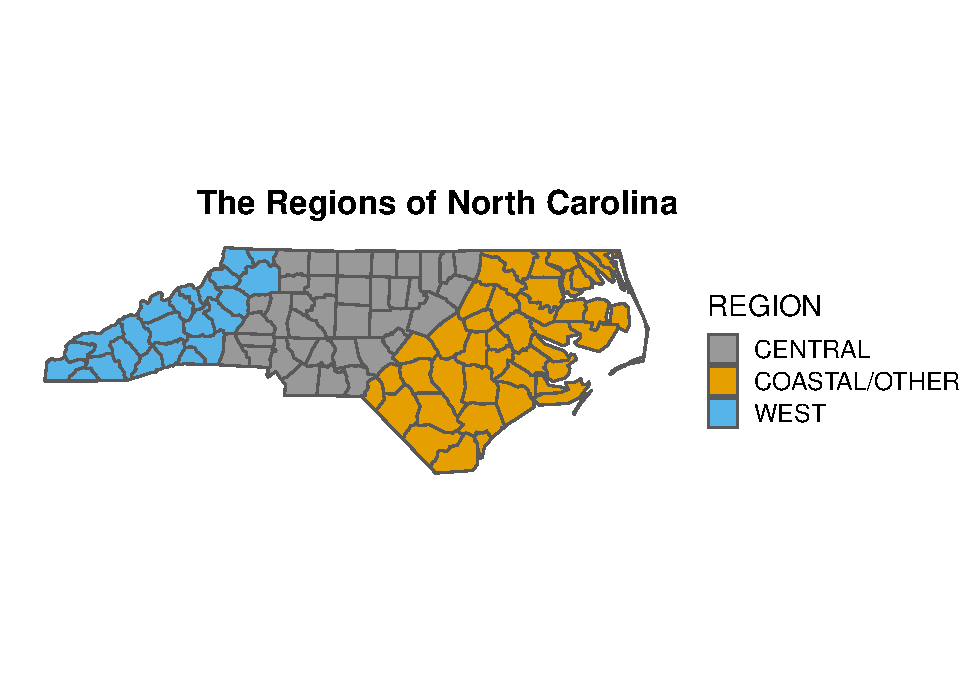
\includegraphics{Bagnard_Gaustad_Hartman_Leung_Lab_3_files/figure-latex/unnamed-chunk-1-1.pdf}

\hypertarget{the-variables}{%
\subsection{The Variables}\label{the-variables}}

The crime\_v2 dataset provided for our study includes 25 variables of
interest, listed below by category.

\begin{center}
\textbf{Data Dictionary}
\end{center}

\begin{longtable}[]{@{}ll@{}}
\toprule
Category & Variable\tabularnewline
\midrule
\endhead
Crime Rate & crmrte\tabularnewline
Geographic & county, west, central\tabularnewline
Demographic & urban, density, pctmin80, pctymle\tabularnewline
Economic - Wage & wcon, wtuc, wtrd, wfir, wser, wmfg, wfed, wsta,
wloc\tabularnewline
Economic - Revenue & taxpc\tabularnewline
Law Enforcment & polpc, prbarr, prbconv, mix\tabularnewline
Judicial/Sentencing & prbpris, avgsen\tabularnewline
Time Period & year\tabularnewline
\bottomrule
\end{longtable}

\begin{center}
Table 1: Data Dictionary
\end{center}

The variables above operationalize the conditions we wish to explore and
their affects on crime.

Chiefly, these break down as follows.

\begin{itemize}
\item
  The Economic variables measure the county's economic activity and
  health (e.g.~opportunity to pursue legal forms of income). These
  variables come in the form of available wages and tax revenue returned
  to the county.
\item
  The Law enforcment variables measure crime statistics as ratios such
  as arrests-to-offenses, convictions-to-arrests, police per capita and
  crime mix.
\item
  The the Judicial variables meaure the outcome of the judicial process
  in the form of prison sentences-to-convictions and average sentence
  length.
\item
  The Demographic variables measure the cultural variability that
  represent the social differences between each county, such as urban vs
  rural and minority populations.
\item
  The Geographic elements are categorical. They represent the ways in
  which the population is segmented by geography.
\end{itemize}

\hypertarget{exploratory-data-analysis-eda}{%
\section{Exploratory Data Analysis
(EDA)}\label{exploratory-data-analysis-eda}}

\hypertarget{data-prep-and-exploration}{%
\subsection{Data Prep and Exploration}\label{data-prep-and-exploration}}

We begin our analysis by loading the data set and performing basic
checks and inspections.

\begin{Shaded}
\begin{Highlighting}[]
\NormalTok{dfCrime =}\StringTok{ }\KeywordTok{read.csv}\NormalTok{(}\StringTok{"crime_v2.csv"}\NormalTok{)}
\KeywordTok{summary}\NormalTok{(dfCrime)}
\end{Highlighting}
\end{Shaded}

\begin{verbatim}
     county           year        crmrte             prbarr       
 Min.   :  1.0   Min.   :87   Min.   :0.005533   Min.   :0.09277  
 1st Qu.: 52.0   1st Qu.:87   1st Qu.:0.020927   1st Qu.:0.20568  
 Median :105.0   Median :87   Median :0.029986   Median :0.27095  
 Mean   :101.6   Mean   :87   Mean   :0.033400   Mean   :0.29492  
 3rd Qu.:152.0   3rd Qu.:87   3rd Qu.:0.039642   3rd Qu.:0.34438  
 Max.   :197.0   Max.   :87   Max.   :0.098966   Max.   :1.09091  
 NA's   :6       NA's   :6    NA's   :6          NA's   :6        
        prbconv      prbpris           avgsen           polpc         
            : 5   Min.   :0.1500   Min.   : 5.380   Min.   :0.000746  
 0.588859022: 2   1st Qu.:0.3648   1st Qu.: 7.340   1st Qu.:0.001231  
 `          : 1   Median :0.4234   Median : 9.100   Median :0.001485  
 0.068376102: 1   Mean   :0.4108   Mean   : 9.647   Mean   :0.001702  
 0.140350997: 1   3rd Qu.:0.4568   3rd Qu.:11.420   3rd Qu.:0.001877  
 0.154451996: 1   Max.   :0.6000   Max.   :20.700   Max.   :0.009054  
 (Other)    :86   NA's   :6        NA's   :6        NA's   :6         
    density            taxpc             west           central      
 Min.   :0.00002   Min.   : 25.69   Min.   :0.0000   Min.   :0.0000  
 1st Qu.:0.54741   1st Qu.: 30.66   1st Qu.:0.0000   1st Qu.:0.0000  
 Median :0.96226   Median : 34.87   Median :0.0000   Median :0.0000  
 Mean   :1.42884   Mean   : 38.06   Mean   :0.2527   Mean   :0.3736  
 3rd Qu.:1.56824   3rd Qu.: 40.95   3rd Qu.:0.5000   3rd Qu.:1.0000  
 Max.   :8.82765   Max.   :119.76   Max.   :1.0000   Max.   :1.0000  
 NA's   :6         NA's   :6        NA's   :6        NA's   :6       
     urban            pctmin80           wcon            wtuc      
 Min.   :0.00000   Min.   : 1.284   Min.   :193.6   Min.   :187.6  
 1st Qu.:0.00000   1st Qu.: 9.845   1st Qu.:250.8   1st Qu.:374.6  
 Median :0.00000   Median :24.312   Median :281.4   Median :406.5  
 Mean   :0.08791   Mean   :25.495   Mean   :285.4   Mean   :411.7  
 3rd Qu.:0.00000   3rd Qu.:38.142   3rd Qu.:314.8   3rd Qu.:443.4  
 Max.   :1.00000   Max.   :64.348   Max.   :436.8   Max.   :613.2  
 NA's   :6         NA's   :6        NA's   :6       NA's   :6      
      wtrd            wfir            wser             wmfg      
 Min.   :154.2   Min.   :170.9   Min.   : 133.0   Min.   :157.4  
 1st Qu.:190.9   1st Qu.:286.5   1st Qu.: 229.7   1st Qu.:288.9  
 Median :203.0   Median :317.3   Median : 253.2   Median :320.2  
 Mean   :211.6   Mean   :322.1   Mean   : 275.6   Mean   :335.6  
 3rd Qu.:225.1   3rd Qu.:345.4   3rd Qu.: 280.5   3rd Qu.:359.6  
 Max.   :354.7   Max.   :509.5   Max.   :2177.1   Max.   :646.9  
 NA's   :6       NA's   :6       NA's   :6        NA's   :6      
      wfed            wsta            wloc            mix         
 Min.   :326.1   Min.   :258.3   Min.   :239.2   Min.   :0.01961  
 1st Qu.:400.2   1st Qu.:329.3   1st Qu.:297.3   1st Qu.:0.08074  
 Median :449.8   Median :357.7   Median :308.1   Median :0.10186  
 Mean   :442.9   Mean   :357.5   Mean   :312.7   Mean   :0.12884  
 3rd Qu.:478.0   3rd Qu.:382.6   3rd Qu.:329.2   3rd Qu.:0.15175  
 Max.   :598.0   Max.   :499.6   Max.   :388.1   Max.   :0.46512  
 NA's   :6       NA's   :6       NA's   :6       NA's   :6        
    pctymle       
 Min.   :0.06216  
 1st Qu.:0.07443  
 Median :0.07771  
 Mean   :0.08396  
 3rd Qu.:0.08350  
 Max.   :0.24871  
 NA's   :6        
\end{verbatim}

First, we note the blank rows which we will remove from the dataset.

\begin{Shaded}
\begin{Highlighting}[]
\KeywordTok{nrow}\NormalTok{(dfCrime)}
\end{Highlighting}
\end{Shaded}

\begin{verbatim}
[1] 97
\end{verbatim}

\begin{Shaded}
\begin{Highlighting}[]
\NormalTok{dfCrime <-}\KeywordTok{na.omit}\NormalTok{(dfCrime) }\CommentTok{# omit the NA rows}
\KeywordTok{nrow}\NormalTok{(dfCrime)}
\end{Highlighting}
\end{Shaded}

\begin{verbatim}
[1] 91
\end{verbatim}

Next, we will inspect the data to see if there are duplicate records

\begin{Shaded}
\begin{Highlighting}[]
\NormalTok{dfCrime[}\KeywordTok{duplicated}\NormalTok{(dfCrime),]}
\end{Highlighting}
\end{Shaded}

\begin{verbatim}
   county year    crmrte   prbarr     prbconv  prbpris avgsen      polpc
89    193   87 0.0235277 0.266055 0.588859022 0.423423   5.86 0.00117887
     density    taxpc west central urban pctmin80     wcon     wtuc
89 0.8138298 28.51783    1       0     0  5.93109 285.8289 480.1948
       wtrd     wfir     wser   wmfg   wfed   wsta   wloc       mix
89 268.3836 365.0196 295.9352 295.63 468.26 337.88 348.74 0.1105016
      pctymle
89 0.07819394
\end{verbatim}

A duplicate row exists. We'll remove it.

\begin{Shaded}
\begin{Highlighting}[]
\NormalTok{dfCrime <-}\StringTok{ }\NormalTok{dfCrime[}\OperatorTok{!}\KeywordTok{duplicated}\NormalTok{(dfCrime),] }\CommentTok{# remove the duplicated row}
\end{Highlighting}
\end{Shaded}

We also see that pbconv is coded as a level. It is not a level but a
ratio. We'll change that now.

\begin{Shaded}
\begin{Highlighting}[]
\NormalTok{dfCrime}\OperatorTok{$}\NormalTok{prbconv<-}\KeywordTok{as.numeric}\NormalTok{(}\KeywordTok{levels}\NormalTok{(dfCrime}\OperatorTok{$}\NormalTok{prbconv))[dfCrime}\OperatorTok{$}\NormalTok{prbconv]}
\end{Highlighting}
\end{Shaded}

We also notice by comparision of pctymle and pctmin80 that one of the
variables is off by a factor of 100. We will divide pctmin80 by 100 so
the two variables share consistent unit terms.

\begin{Shaded}
\begin{Highlighting}[]
\NormalTok{dfCrime}\OperatorTok{$}\NormalTok{pctmin80<-dfCrime}\OperatorTok{$}\NormalTok{pctmin80}\OperatorTok{/}\DecValTok{100}
\end{Highlighting}
\end{Shaded}

County was expressed as a number. However, it is a categorical variable
and we will convert it to a factor instead.

\begin{Shaded}
\begin{Highlighting}[]
\NormalTok{dfCrime}\OperatorTok{$}\NormalTok{county<-}\KeywordTok{as.factor}\NormalTok{(dfCrime}\OperatorTok{$}\NormalTok{county)}
\end{Highlighting}
\end{Shaded}

Next we inspect the indicator variables to see if they were coded
correctly.

\begin{Shaded}
\begin{Highlighting}[]
\NormalTok{dfCrime }\OperatorTok\StringTok{ }\KeywordTok{group_by}\NormalTok{(west, central) }\OperatorTok\StringTok{ }\KeywordTok{tally}\NormalTok{()}
\end{Highlighting}
\end{Shaded}

\begin{verbatim}
# A tibble: 4 x 3
# Groups:   west [2]
   west central     n
  <int>   <int> <int>
1     0       0    35
2     0       1    33
3     1       0    21
4     1       1     1
\end{verbatim}

\begin{Shaded}
\begin{Highlighting}[]
\NormalTok{dfCrime }\OperatorTok
\KeywordTok{filter}\NormalTok{(west }\OperatorTok{==}\DecValTok{1} \OperatorTok{&}\StringTok{ }\NormalTok{central }\OperatorTok{==}\DecValTok{1}\NormalTok{)}
\end{Highlighting}
\end{Shaded}

\begin{verbatim}
  county year    crmrte   prbarr prbconv  prbpris avgsen      polpc
1     71   87 0.0544061 0.243119 0.22959 0.379175  11.29 0.00207028
   density    taxpc west central urban pctmin80     wcon     wtuc     wtrd
1 4.834734 31.53658    1       1     0  0.13315 291.4508 595.3719 240.3673
      wfir     wser   wmfg   wfed   wsta   wloc       mix    pctymle
1 348.0254 295.2301 358.95 509.43 359.11 339.58 0.1018608 0.07939028
\end{verbatim}

One county was either mis-coded (with west=1 and central=1), or the
county truly belongs to both regions. However, this association is very
unlikely as the proper coding technique is to widen the data and
introduce indicator variables for each category. The coding technique
does not allow membership in both categories, and a separate third
indicator variable would have been created instead.

We will need further analysis on this datapoint to assess proper
treatment options.

For now, we will encode a new region variable that does place the
datapoint in its own category.

\begin{Shaded}
\begin{Highlighting}[]
\CommentTok{#Map central and west to a region code, and create a new category for other}
\CommentTok{# Note that county 71 has both western and central codes}
\NormalTok{dfCrime}\OperatorTok{$}\NormalTok{region <-}\StringTok{ }\KeywordTok{case_when}\NormalTok{ (}
\NormalTok{            (dfCrime}\OperatorTok{$}\NormalTok{central }\OperatorTok{==}\DecValTok{0} \OperatorTok{&}\StringTok{ }\NormalTok{dfCrime}\OperatorTok{$}\NormalTok{west }\OperatorTok{==}\DecValTok{0}\NormalTok{) }\OperatorTok{~}\StringTok{ }\DecValTok{0}\NormalTok{, }\CommentTok{#Eastern, Coastal, Other}
\NormalTok{            (dfCrime}\OperatorTok{$}\NormalTok{central }\OperatorTok{==}\DecValTok{0} \OperatorTok{&}\StringTok{ }\NormalTok{dfCrime}\OperatorTok{$}\NormalTok{west }\OperatorTok{==}\DecValTok{1}\NormalTok{) }\OperatorTok{~}\StringTok{ }\DecValTok{1}\NormalTok{, }\CommentTok{#Western}
\NormalTok{            (dfCrime}\OperatorTok{$}\NormalTok{central }\OperatorTok{==}\DecValTok{1} \OperatorTok{&}\StringTok{ }\NormalTok{dfCrime}\OperatorTok{$}\NormalTok{west }\OperatorTok{==}\DecValTok{0}\NormalTok{) }\OperatorTok{~}\StringTok{ }\DecValTok{2}\NormalTok{, }\CommentTok{#Central}
\NormalTok{            (dfCrime}\OperatorTok{$}\NormalTok{central }\OperatorTok{==}\DecValTok{1} \OperatorTok{&}\StringTok{ }\NormalTok{dfCrime}\OperatorTok{$}\NormalTok{west }\OperatorTok{==}\DecValTok{1}\NormalTok{) }\OperatorTok{~}\StringTok{ }\DecValTok{3} \CommentTok{#Central-Western county?}
\NormalTok{        )}
\NormalTok{dfCrime}\OperatorTok{$}\NormalTok{regcode =}
\StringTok{            }\KeywordTok{factor}\NormalTok{( dfCrime}\OperatorTok{$}\NormalTok{region , }\DataTypeTok{levels =} \DecValTok{0}\OperatorTok{:}\DecValTok{3}\NormalTok{ , }\DataTypeTok{labels =}
                    \KeywordTok{c}\NormalTok{( }\StringTok{'Other'}\NormalTok{,}
                       \StringTok{'West'}\NormalTok{,}
                       \StringTok{'Central'}\NormalTok{,}
                       \StringTok{'CW'}\NormalTok{)}
\NormalTok{                   )}
\end{Highlighting}
\end{Shaded}

We will also introduce an indicator variable for counties located in the
``other'' region not in west or central

\begin{Shaded}
\begin{Highlighting}[]
\NormalTok{dfCrime}\OperatorTok{$}\NormalTok{other <-}\StringTok{ }\KeywordTok{ifelse}\NormalTok{((dfCrime}\OperatorTok{$}\NormalTok{central }\OperatorTok{==}\DecValTok{0} \OperatorTok{&}\StringTok{ }\NormalTok{dfCrime}\OperatorTok{$}\NormalTok{west }\OperatorTok{==}\DecValTok{0}\NormalTok{), }\DecValTok{1}\NormalTok{, }\DecValTok{0}\NormalTok{)}
\end{Highlighting}
\end{Shaded}

And we'll add an indicator variable to serve as complement to the urban
indicator variable and call this `nonurban'

\begin{Shaded}
\begin{Highlighting}[]
\NormalTok{dfCrime}\OperatorTok{$}\NormalTok{nonurban <-}\StringTok{ }\KeywordTok{ifelse}\NormalTok{((dfCrime}\OperatorTok{$}\NormalTok{urban}\OperatorTok{==}\DecValTok{0}\NormalTok{), }\DecValTok{1}\NormalTok{, }\DecValTok{0}\NormalTok{)}
\end{Highlighting}
\end{Shaded}

By way of the 1980 Census fact sheet, we discover the urban field is an
encoding for SMSA (Standard Metropolitan Statistical Areas).
\url{https://www2.census.gov/prod2/decennial/documents/1980/1980censusofpopu8011uns_bw.pdf}
The value is 1 if the county is inside a metropolitan area. Otherwise,
if the county is outside a metropolitan area, the value is 0.

We create a metro factor variable to better describe this feature for
visualization purposes.

\begin{Shaded}
\begin{Highlighting}[]
\CommentTok{# create factor for SMSA (standard metropolitan statistical areas) with two levels}
\CommentTok{# (inside or outside)}
\CommentTok{#    https://www2.census.gov/prod2/decennial/documents/1980/1980censusofpopu8011uns_bw.pdf}
\NormalTok{dfCrime}\OperatorTok{$}\NormalTok{metro =}
\StringTok{            }\KeywordTok{factor}\NormalTok{( dfCrime}\OperatorTok{$}\NormalTok{urban , }\DataTypeTok{levels =} \DecValTok{0}\OperatorTok{:}\DecValTok{1}\NormalTok{ , }\DataTypeTok{labels =}
                    \KeywordTok{c}\NormalTok{( }\StringTok{'Outside Metro'}\NormalTok{,}
                       \StringTok{'Inside Metro'}
\NormalTok{                      )}
\NormalTok{                   )}
\end{Highlighting}
\end{Shaded}

\hypertarget{outlier-analysis}{%
\subsubsection{Outlier Analysis}\label{outlier-analysis}}

Now we will visualize our numerical variables in boxplots and use our
categorical variables to highlight differences.

\begin{Shaded}
\begin{Highlighting}[]
\CommentTok{#Plot of the economic and tax related variables vs crmrte}
\NormalTok{q1<-}\KeywordTok{ggplot}\NormalTok{(}\DataTypeTok{data =}\NormalTok{ dfCrime, }\KeywordTok{aes}\NormalTok{(}\DataTypeTok{y =}\NormalTok{ wcon, }\DataTypeTok{color =}\NormalTok{ regcode)) }\OperatorTok{+}
\StringTok{      }\KeywordTok{geom_boxplot}\NormalTok{()}
\NormalTok{q2<-}\KeywordTok{ggplot}\NormalTok{(}\DataTypeTok{data =}\NormalTok{ dfCrime, }\KeywordTok{aes}\NormalTok{(}\DataTypeTok{y =}\NormalTok{ wtuc, }\DataTypeTok{color =}\NormalTok{ regcode)) }\OperatorTok{+}
\StringTok{      }\KeywordTok{geom_boxplot}\NormalTok{()}
\NormalTok{q3<-}\KeywordTok{ggplot}\NormalTok{(}\DataTypeTok{data =}\NormalTok{ dfCrime, }\KeywordTok{aes}\NormalTok{(}\DataTypeTok{y =}\NormalTok{ wtrd, }\DataTypeTok{color =}\NormalTok{ regcode)) }\OperatorTok{+}
\StringTok{      }\KeywordTok{geom_boxplot}\NormalTok{()}
\NormalTok{q4<-}\KeywordTok{ggplot}\NormalTok{(}\DataTypeTok{data =}\NormalTok{ dfCrime, }\KeywordTok{aes}\NormalTok{(}\DataTypeTok{y =}\NormalTok{ wfir, }\DataTypeTok{color =}\NormalTok{ regcode)) }\OperatorTok{+}
\StringTok{      }\KeywordTok{geom_boxplot}\NormalTok{()}
\NormalTok{q5<-}\KeywordTok{ggplot}\NormalTok{(}\DataTypeTok{data =}\NormalTok{ dfCrime, }\KeywordTok{aes}\NormalTok{(}\DataTypeTok{y =}\NormalTok{ wser, }\DataTypeTok{color =}\NormalTok{ regcode)) }\OperatorTok{+}
\StringTok{      }\KeywordTok{geom_boxplot}\NormalTok{()}
\NormalTok{q6<-}\KeywordTok{ggplot}\NormalTok{(}\DataTypeTok{data =}\NormalTok{ dfCrime, }\KeywordTok{aes}\NormalTok{(}\DataTypeTok{y =}\NormalTok{ wmfg, }\DataTypeTok{color =}\NormalTok{ regcode)) }\OperatorTok{+}
\StringTok{      }\KeywordTok{geom_boxplot}\NormalTok{()}
\NormalTok{q7<-}\KeywordTok{ggplot}\NormalTok{(}\DataTypeTok{data =}\NormalTok{ dfCrime, }\KeywordTok{aes}\NormalTok{(}\DataTypeTok{y =}\NormalTok{ wfed, }\DataTypeTok{color =}\NormalTok{ regcode)) }\OperatorTok{+}
\StringTok{      }\KeywordTok{geom_boxplot}\NormalTok{()}
\NormalTok{q8<-}\KeywordTok{ggplot}\NormalTok{(}\DataTypeTok{data =}\NormalTok{ dfCrime, }\KeywordTok{aes}\NormalTok{(}\DataTypeTok{y =}\NormalTok{ wsta, }\DataTypeTok{color =}\NormalTok{ regcode)) }\OperatorTok{+}
\StringTok{      }\KeywordTok{geom_boxplot}\NormalTok{()}
\NormalTok{q9<-}\KeywordTok{ggplot}\NormalTok{(}\DataTypeTok{data =}\NormalTok{ dfCrime, }\KeywordTok{aes}\NormalTok{(}\DataTypeTok{y =}\NormalTok{ wloc, }\DataTypeTok{color =}\NormalTok{ regcode)) }\OperatorTok{+}
\StringTok{      }\KeywordTok{geom_boxplot}\NormalTok{()}
\NormalTok{q10<-}\KeywordTok{ggplot}\NormalTok{(}\DataTypeTok{data =}\NormalTok{ dfCrime, }\KeywordTok{aes}\NormalTok{(}\DataTypeTok{y =}\NormalTok{ taxpc, }\DataTypeTok{color =}\NormalTok{ regcode)) }\OperatorTok{+}
\StringTok{      }\KeywordTok{geom_boxplot}\NormalTok{()}
\KeywordTok{grid.arrange}\NormalTok{(q1, q2, q3, q4, }\DataTypeTok{ncol=}\DecValTok{2}\NormalTok{)}
\end{Highlighting}
\end{Shaded}

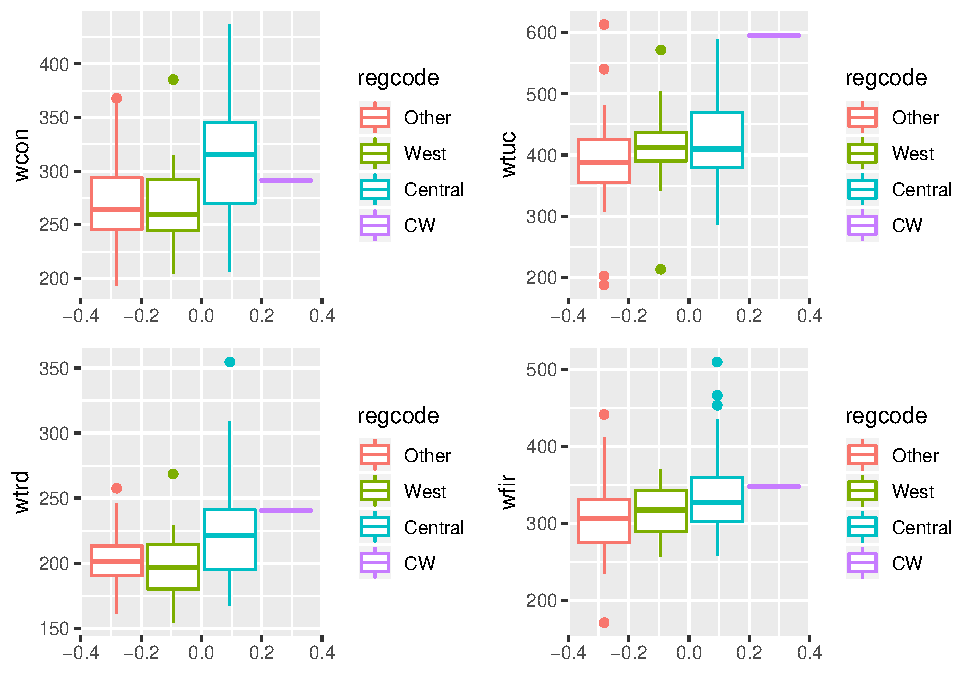
\includegraphics{Bagnard_Gaustad_Hartman_Leung_Lab_3_files/figure-latex/unnamed-chunk-15-1.pdf}

\begin{Shaded}
\begin{Highlighting}[]
\KeywordTok{grid.arrange}\NormalTok{(q5, q6, q7, q8, q9, q10, }\DataTypeTok{ncol=}\DecValTok{2}\NormalTok{)}
\end{Highlighting}
\end{Shaded}

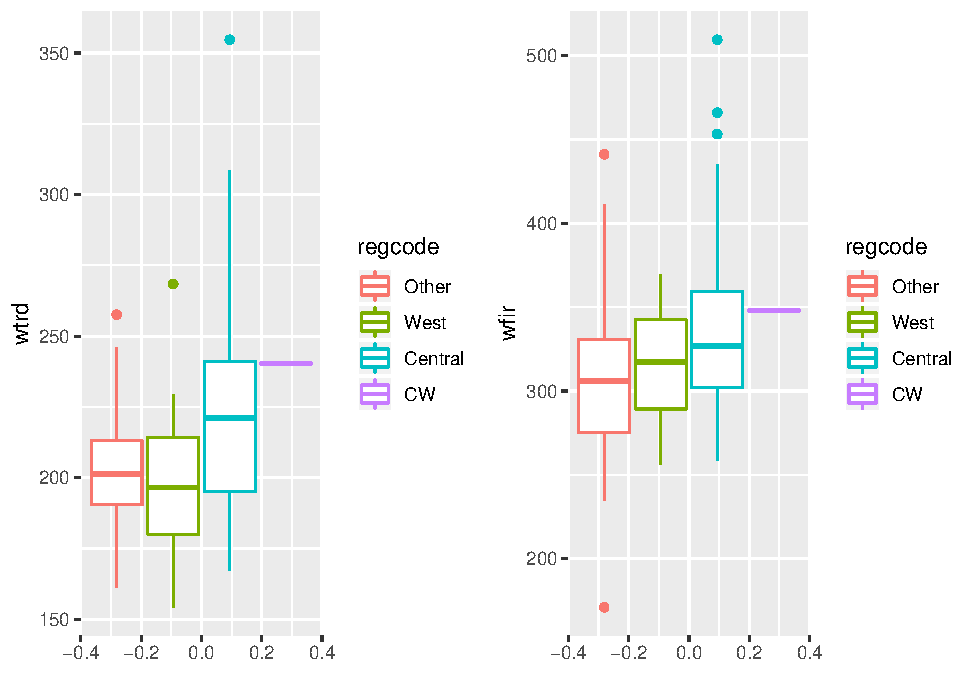
\includegraphics{Bagnard_Gaustad_Hartman_Leung_Lab_3_files/figure-latex/unnamed-chunk-15-2.pdf}

We note in the comparison above wser appears to have an extreme outlier.

Other variables show outliers as well, but not as extreme. We will
determine if any of these points have leverage or influence in model
specification.

For now, we will dig deeper into wser to confirm our understanding of
the variable after the visual inspection.

\begin{Shaded}
\begin{Highlighting}[]
\NormalTok{dfCrime }\OperatorTok
\KeywordTok{filter}\NormalTok{(wser }\OperatorTok{>}\StringTok{ }\DecValTok{2000}\NormalTok{) }\OperatorTok
\KeywordTok{select}\NormalTok{(county, wser)}
\end{Highlighting}
\end{Shaded}

\begin{verbatim}
  county     wser
1    185 2177.068
\end{verbatim}

This average service wage is in extreme excess based on what we know
about the 1980s and every wage recorded in comparison. A review of the
detailed population statistics describing mean wage per industry (table
231) confirms this.
\url{https://www2.census.gov/prod2/decennial/documents/1980/1980censusofpopu801352uns_bw.pdf}

We have identified our first outlier. Outliers affect our ability to
estimate statistics, resulting in overestimated or underestimated
values. Outliers can be due to a number of factors such as response
errors and data entry errors. Outliers will introduce bias into our
estimates and they need to be addressed during the analysis phase. The
treatment remedies include three options.

1 Trimming - \emph{remove} outliers from the dataset based on a maxima
or minima from the mean.

2 Winsorization - \emph{replace} extreme values with the next available
point in the range so they fall at the edge of the distribution

3 Imputation - \emph{recode} outliers by calculating the mean of the
sample, or by applying a regression model to predict the missing value

Trimming an entire county is not a preferred treatment as we may lose
valuable information in other fields.

Winsorization is a symmetric process that will replace \emph{all} of our
smallest and largest data values in the sample. This is not a preferred
treatment as we may again lose valuable information, especially when we
only seek to replace values that are a result of a coding error.

Imputation recodes the data point using a predictive model derived from
the sample. Multiple imputations are performed on the data to account
for uncertainty, and each imputed result set is analyzed for its
distribution. Then, the mean, mode or median can be chosen from this
distribution as the replacement.

We note that none of these methods are ideal. We would be better suited
if we could track the nature of the mistake and recode the value from
underlying data. Since we do not have access to the underlying data rom
which this sample set was derived, we must utilize one of the methods
above in order to continue with our analysis. We favor the imputation
method as it reduces the chances of us losing valuable data.
Fortunately, a number of packages are available in R that predict a
replacement value through imputation A commonly used library for
imputation can be found in the Hmisc package which we will use for our
outlier treatment.

A full discussion of treatment methods can be found here:
\url{http://www.asasrms.org/Proceedings/y2004/files/Jsm2004-000559.pdf}

Now we will begin our treatment.

\begin{Shaded}
\begin{Highlighting}[]
\NormalTok{dfCrime}\OperatorTok{$}\NormalTok{wser[}\KeywordTok{which}\NormalTok{(dfCrime}\OperatorTok{$}\NormalTok{county}\OperatorTok{==}\DecValTok{185}\NormalTok{)]<-}\OtherTok{NA} \CommentTok{# set the value to NA so it will be imputed}
\end{Highlighting}
\end{Shaded}

\begin{Shaded}
\begin{Highlighting}[]
\NormalTok{impute_arg <-}\StringTok{ }\KeywordTok{aregImpute}\NormalTok{(}\OperatorTok{~}\StringTok{ }\NormalTok{crmrte }\OperatorTok{+}\StringTok{  }\NormalTok{urban }\OperatorTok{+}\StringTok{ }\NormalTok{central }\OperatorTok{+}\StringTok{ }\NormalTok{west }\OperatorTok{+}\StringTok{ }\NormalTok{other }\OperatorTok{+}
\StringTok{                         }\NormalTok{prbarr }\OperatorTok{+}\StringTok{ }\NormalTok{prbconv }\OperatorTok{+}\StringTok{ }\NormalTok{prbpris }\OperatorTok{+}\StringTok{ }\NormalTok{avgsen }\OperatorTok{+}\StringTok{ }\NormalTok{polpc }\OperatorTok{+}
\StringTok{                         }\NormalTok{density }\OperatorTok{+}\StringTok{ }\NormalTok{taxpc }\OperatorTok{+}\StringTok{ }\NormalTok{pctmin80 }\OperatorTok{+}\StringTok{ }\NormalTok{wcon }\OperatorTok{+}\StringTok{ }\NormalTok{wtuc }\OperatorTok{+}
\StringTok{                         }\NormalTok{wtrd }\OperatorTok{+}\StringTok{ }\NormalTok{wfir }\OperatorTok{+}\StringTok{ }\NormalTok{wser }\OperatorTok{+}\StringTok{ }\NormalTok{wmfg }\OperatorTok{+}\StringTok{ }\NormalTok{wfed }\OperatorTok{+}\StringTok{ }\NormalTok{wsta }\OperatorTok{+}\StringTok{ }\NormalTok{wloc }\OperatorTok{+}
\StringTok{                         }\NormalTok{mix }\OperatorTok{+}\StringTok{ }\NormalTok{pctymle, }\DataTypeTok{data =}\NormalTok{ dfCrime, }\DataTypeTok{match=}\StringTok{"weighted"}\NormalTok{,}
                         \DataTypeTok{nk=}\DecValTok{3}\NormalTok{, }\DataTypeTok{B=}\DecValTok{10}\NormalTok{, }\DataTypeTok{n.impute =} \DecValTok{100}\NormalTok{)}
\end{Highlighting}
\end{Shaded}

\begin{Shaded}
\begin{Highlighting}[]
\CommentTok{#Review R-squares for Predicting Non-Missing Values for Each Variable.}
\CommentTok{#A high R-square reveals a high degree of confidence in being able to predict}
\NormalTok{impute_arg}\OperatorTok{$}\NormalTok{rsq}
\end{Highlighting}
\end{Shaded}

\begin{verbatim}
     wser 
0.9252622 
\end{verbatim}

\begin{Shaded}
\begin{Highlighting}[]
\CommentTok{# Review Distribution of Values from Each Imputation}
\KeywordTok{table}\NormalTok{(impute_arg}\OperatorTok{$}\NormalTok{imputed}\OperatorTok{$}\NormalTok{wser)}
\end{Highlighting}
\end{Shaded}

\begin{verbatim}

133.0430603 172.4732666 172.6280975 182.0196228 192.3076935 204.3792114 
         11           5           1           3           1           1 
 206.281601 209.6972198 213.5821533 215.1933289 223.8502197 229.0150757 
          3           1           1           1           1           2 
230.4980621 231.3615112 246.0152435 247.6290894 253.2280579 274.1774597 
          1           1           1           2           1          62 
296.8490906 
          1 
\end{verbatim}

We note from the distribution above we see a mode appear from the
multiple imputation trials. While taking the mode may sufficient for
replacement (particularly for categorical values), to be conservative,
we will reassign this value using the mean value from the prediction
trials.

\begin{Shaded}
\begin{Highlighting}[]
\NormalTok{dfCrime}\OperatorTok{$}\NormalTok{wser[}\KeywordTok{which}\NormalTok{(dfCrime}\OperatorTok{$}\NormalTok{county}\OperatorTok{==}\DecValTok{185}\NormalTok{)]<-}\KeywordTok{mean}\NormalTok{(impute_arg}\OperatorTok{$}\NormalTok{imputed}\OperatorTok{$}\NormalTok{wser)}
\CommentTok{#Confirm assigned value}
\NormalTok{dfCrime}\OperatorTok{$}\NormalTok{wser[}\KeywordTok{which}\NormalTok{(dfCrime}\OperatorTok{$}\NormalTok{county}\OperatorTok{==}\DecValTok{185}\NormalTok{)]}
\end{Highlighting}
\end{Shaded}

\begin{verbatim}
[1] 241.3262
\end{verbatim}

We turn our examination now to the criminal justice variables.

\begin{Shaded}
\begin{Highlighting}[]
\CommentTok{#Plot of the criminal justice and law enforcment related variables vs crmrte}
\NormalTok{q1<-}\KeywordTok{ggplot}\NormalTok{(}\DataTypeTok{data =}\NormalTok{ dfCrime, }\KeywordTok{aes}\NormalTok{(}\DataTypeTok{y =}\NormalTok{ prbarr, }\DataTypeTok{color =}\NormalTok{ regcode)) }\OperatorTok{+}
\StringTok{      }\KeywordTok{geom_boxplot}\NormalTok{()}
\NormalTok{q2<-}\KeywordTok{ggplot}\NormalTok{(}\DataTypeTok{data =}\NormalTok{ dfCrime, }\KeywordTok{aes}\NormalTok{(}\DataTypeTok{y =}\NormalTok{ prbconv, }\DataTypeTok{color =}\NormalTok{ regcode)) }\OperatorTok{+}
\StringTok{      }\KeywordTok{geom_boxplot}\NormalTok{()}
\NormalTok{q3<-}\KeywordTok{ggplot}\NormalTok{(}\DataTypeTok{data =}\NormalTok{ dfCrime, }\KeywordTok{aes}\NormalTok{(}\DataTypeTok{y =}\NormalTok{ prbpris, }\DataTypeTok{color =}\NormalTok{ regcode)) }\OperatorTok{+}
\StringTok{      }\KeywordTok{geom_boxplot}\NormalTok{()}
\NormalTok{q4<-}\KeywordTok{ggplot}\NormalTok{(}\DataTypeTok{data =}\NormalTok{ dfCrime, }\KeywordTok{aes}\NormalTok{(}\DataTypeTok{y =}\NormalTok{ avgsen, }\DataTypeTok{color =}\NormalTok{ regcode)) }\OperatorTok{+}
\StringTok{      }\KeywordTok{geom_boxplot}\NormalTok{()}
\NormalTok{q5<-}\KeywordTok{ggplot}\NormalTok{(}\DataTypeTok{data =}\NormalTok{ dfCrime, }\KeywordTok{aes}\NormalTok{(}\DataTypeTok{y =}\NormalTok{ polpc, }\DataTypeTok{color =}\NormalTok{ regcode)) }\OperatorTok{+}
\StringTok{      }\KeywordTok{geom_boxplot}\NormalTok{()}
\NormalTok{q6<-}\KeywordTok{ggplot}\NormalTok{(}\DataTypeTok{data =}\NormalTok{ dfCrime, }\KeywordTok{aes}\NormalTok{(}\DataTypeTok{y =}\NormalTok{ mix, }\DataTypeTok{color =}\NormalTok{ regcode)) }\OperatorTok{+}
\StringTok{      }\KeywordTok{geom_boxplot}\NormalTok{()}

\KeywordTok{grid.arrange}\NormalTok{(q1, q2, }\DataTypeTok{ncol=}\DecValTok{2}\NormalTok{)}
\end{Highlighting}
\end{Shaded}

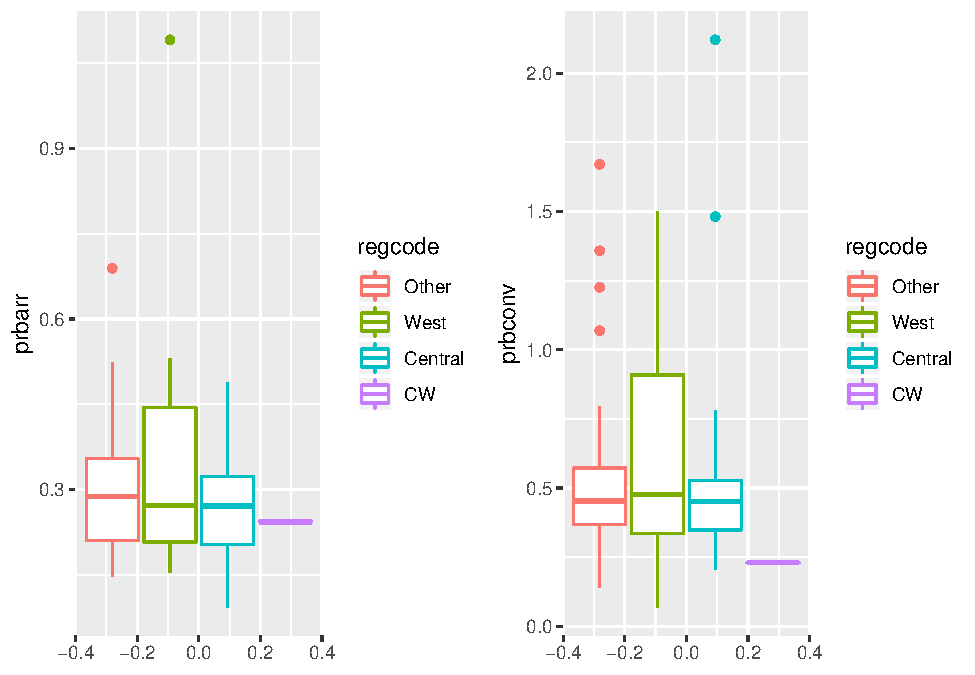
\includegraphics{Bagnard_Gaustad_Hartman_Leung_Lab_3_files/figure-latex/unnamed-chunk-22-1.pdf}

\begin{Shaded}
\begin{Highlighting}[]
\KeywordTok{grid.arrange}\NormalTok{(q3, q4, q5, q6, }\DataTypeTok{ncol=}\DecValTok{2}\NormalTok{)}
\end{Highlighting}
\end{Shaded}

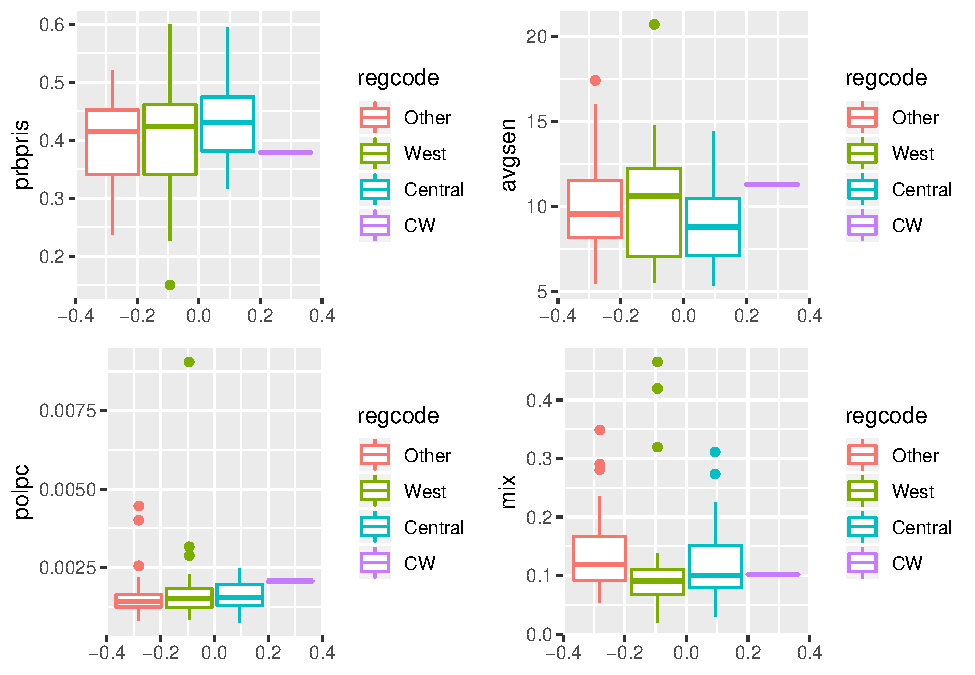
\includegraphics{Bagnard_Gaustad_Hartman_Leung_Lab_3_files/figure-latex/unnamed-chunk-22-2.pdf}

The criminal justice and law enforcement variables show evidence of
outliers, notably, prbarr and polpc appear to have extreme data points.

We will suspend comment on prbarr for now, but, we will comment on the
extreme outlier value of polpc which is .009. Based on records
describing the US population on police officers per capita, the highest
police per capita on record for all United States counties is .007. This
high value occurs in Atlantic City, NJ.
\url{https://www.governing.com/gov-data/safety-justice/police-officers-per-capita-rates-employment-for-city-departments.html}

The datapoint in our sample set is an error, and we will impute it's
replacement.

\begin{Shaded}
\begin{Highlighting}[]
\NormalTok{dfCrime}\OperatorTok{$}\NormalTok{polpc[}\KeywordTok{which}\NormalTok{(dfCrime}\OperatorTok{$}\NormalTok{county}\OperatorTok{==}\DecValTok{115}\NormalTok{)]<-}\OtherTok{NA} \CommentTok{# set the value to NA so it will be imputed}
\end{Highlighting}
\end{Shaded}

\begin{Shaded}
\begin{Highlighting}[]
\NormalTok{impute_arg <-}\StringTok{ }\KeywordTok{aregImpute}\NormalTok{(}\OperatorTok{~}\StringTok{ }\NormalTok{crmrte }\OperatorTok{+}\StringTok{  }\NormalTok{urban }\OperatorTok{+}\StringTok{ }\NormalTok{central }\OperatorTok{+}\StringTok{ }\NormalTok{west }\OperatorTok{+}\StringTok{ }\NormalTok{other }\OperatorTok{+}
\StringTok{                         }\NormalTok{prbarr }\OperatorTok{+}\StringTok{ }\NormalTok{prbconv }\OperatorTok{+}\StringTok{ }\NormalTok{prbpris }\OperatorTok{+}\StringTok{ }\NormalTok{avgsen }\OperatorTok{+}\StringTok{ }\NormalTok{polpc }\OperatorTok{+}
\StringTok{                         }\NormalTok{density }\OperatorTok{+}\StringTok{ }\NormalTok{taxpc }\OperatorTok{+}\StringTok{ }\NormalTok{pctmin80 }\OperatorTok{+}\StringTok{ }\NormalTok{wcon }\OperatorTok{+}\StringTok{ }\NormalTok{wtuc }\OperatorTok{+}
\StringTok{                         }\NormalTok{wtrd }\OperatorTok{+}\StringTok{ }\NormalTok{wfir }\OperatorTok{+}\StringTok{ }\NormalTok{wser }\OperatorTok{+}\StringTok{ }\NormalTok{wmfg }\OperatorTok{+}\StringTok{ }\NormalTok{wfed }\OperatorTok{+}\StringTok{ }\NormalTok{wsta }\OperatorTok{+}\StringTok{ }\NormalTok{wloc }\OperatorTok{+}
\StringTok{                         }\NormalTok{mix }\OperatorTok{+}\StringTok{ }\NormalTok{pctymle, }\DataTypeTok{data =}\NormalTok{ dfCrime, }\DataTypeTok{match=}\StringTok{"weighted"}\NormalTok{,}
                         \DataTypeTok{nk=}\DecValTok{3}\NormalTok{, }\DataTypeTok{B=}\DecValTok{10}\NormalTok{, }\DataTypeTok{n.impute =} \DecValTok{100}\NormalTok{)}
\end{Highlighting}
\end{Shaded}

\begin{Shaded}
\begin{Highlighting}[]
\KeywordTok{paste}\NormalTok{(}\StringTok{"R-squares for Predicting Non-Missing Values for Each Variable"}\NormalTok{)}
\end{Highlighting}
\end{Shaded}

\begin{verbatim}
[1] "R-squares for Predicting Non-Missing Values for Each Variable"
\end{verbatim}

\begin{Shaded}
\begin{Highlighting}[]
\NormalTok{impute_arg}\OperatorTok{$}\NormalTok{rsq}
\end{Highlighting}
\end{Shaded}

\begin{verbatim}
    polpc 
0.9158124 
\end{verbatim}

\begin{Shaded}
\begin{Highlighting}[]
\KeywordTok{paste}\NormalTok{(}\StringTok{"Predicted values"}\NormalTok{)}
\end{Highlighting}
\end{Shaded}

\begin{verbatim}
[1] "Predicted values"
\end{verbatim}

\begin{Shaded}
\begin{Highlighting}[]
\KeywordTok{mean}\NormalTok{(impute_arg}\OperatorTok{$}\NormalTok{imputed}\OperatorTok{$}\NormalTok{polpc)}
\end{Highlighting}
\end{Shaded}

\begin{verbatim}
[1] 0.002764928
\end{verbatim}

We will reassign this value using the mean from the trials.

\begin{Shaded}
\begin{Highlighting}[]
\NormalTok{dfCrime}\OperatorTok{$}\NormalTok{polpc[}\KeywordTok{which}\NormalTok{(dfCrime}\OperatorTok{$}\NormalTok{county}\OperatorTok{==}\DecValTok{115}\NormalTok{)]<-}\KeywordTok{mean}\NormalTok{(impute_arg}\OperatorTok{$}\NormalTok{imputed}\OperatorTok{$}\NormalTok{polpc)}
\end{Highlighting}
\end{Shaded}

We continue our examination and look into the demographic data next.

\begin{Shaded}
\begin{Highlighting}[]
\CommentTok{#plot of demographic information for counties Outside and Inside the metro areas}
\CommentTok{# population density, percent minority, percent young male}

\KeywordTok{ggplot}\NormalTok{(}\DataTypeTok{data =}\NormalTok{ dfCrime, }\KeywordTok{aes}\NormalTok{(}\DataTypeTok{y =}\NormalTok{ density, }\DataTypeTok{color =}\NormalTok{ regcode)) }\OperatorTok{+}
\StringTok{      }\KeywordTok{geom_boxplot}\NormalTok{() }\OperatorTok{+}\StringTok{ }\KeywordTok{facet_wrap}\NormalTok{(}\OperatorTok{~}\StringTok{ }\NormalTok{metro)}
\end{Highlighting}
\end{Shaded}

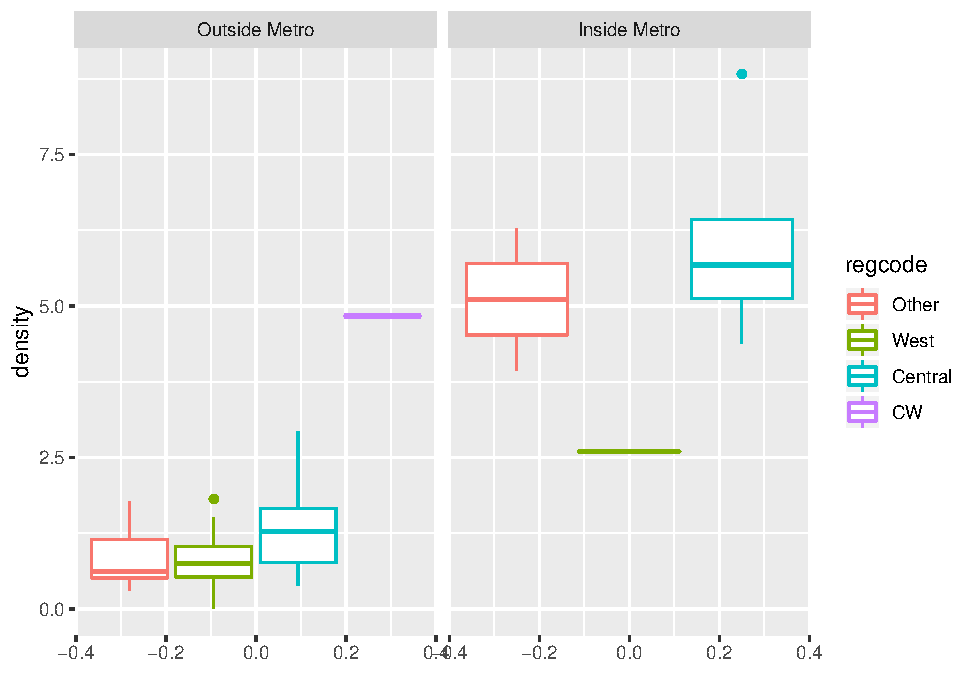
\includegraphics{Bagnard_Gaustad_Hartman_Leung_Lab_3_files/figure-latex/unnamed-chunk-27-1.pdf}

\begin{Shaded}
\begin{Highlighting}[]
\KeywordTok{ggplot}\NormalTok{(}\DataTypeTok{data =}\NormalTok{ dfCrime, }\KeywordTok{aes}\NormalTok{(}\DataTypeTok{y =}\NormalTok{ pctmin80, }\DataTypeTok{color =}\NormalTok{ regcode)) }\OperatorTok{+}
\StringTok{      }\KeywordTok{geom_boxplot}\NormalTok{() }\OperatorTok{+}\StringTok{ }\KeywordTok{facet_wrap}\NormalTok{(}\OperatorTok{~}\StringTok{ }\NormalTok{metro)}
\end{Highlighting}
\end{Shaded}

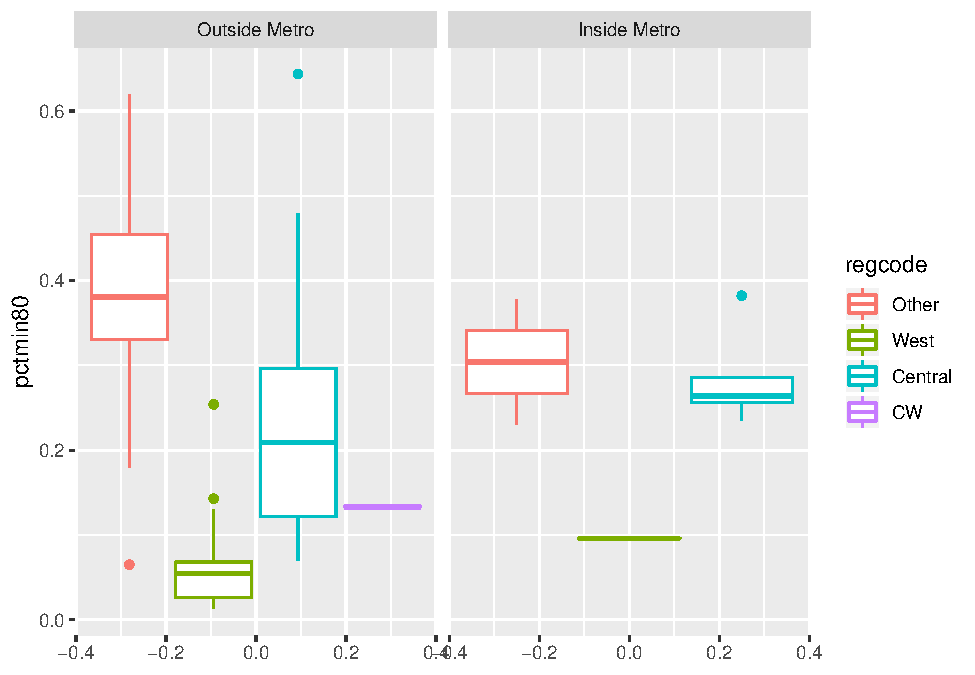
\includegraphics{Bagnard_Gaustad_Hartman_Leung_Lab_3_files/figure-latex/unnamed-chunk-27-2.pdf}

\begin{Shaded}
\begin{Highlighting}[]
\KeywordTok{ggplot}\NormalTok{(}\DataTypeTok{data =}\NormalTok{ dfCrime, }\KeywordTok{aes}\NormalTok{(}\DataTypeTok{y =}\NormalTok{ pctymle, }\DataTypeTok{color =}\NormalTok{ regcode)) }\OperatorTok{+}
\StringTok{      }\KeywordTok{geom_boxplot}\NormalTok{() }\OperatorTok{+}\StringTok{ }\KeywordTok{facet_wrap}\NormalTok{(}\OperatorTok{~}\StringTok{ }\NormalTok{metro)}
\end{Highlighting}
\end{Shaded}

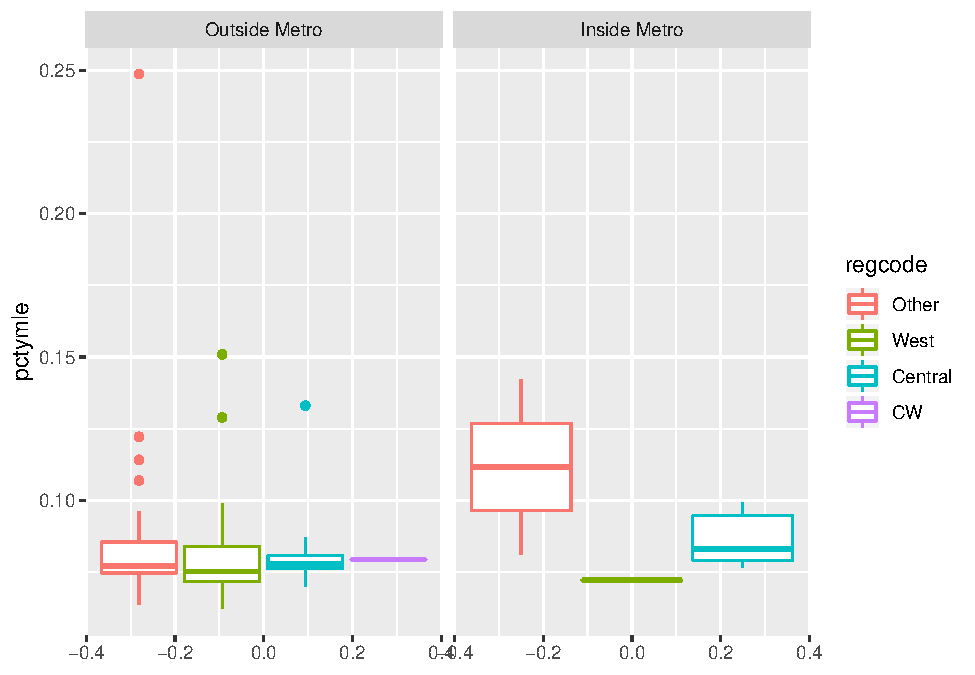
\includegraphics{Bagnard_Gaustad_Hartman_Leung_Lab_3_files/figure-latex/unnamed-chunk-27-3.pdf}

More outliers are observed in demographic information. Looking at
pctymle, in one county it is nearly 25\% young male from 16-24, which
seems quite high. However, this can be explained as coming from county
with a large college town population. Specifically, Appalachian State
University in Watauga County
(\url{https://en.wikipedia.org/wiki/Watauga_County,_North_Carolina}),
where the presense of the university notably affects the overall age
distribution and our median age. This is further confirmed in county
estimate records located here:
\url{https://www.osbm.nc.gov/demog/county-estimates}.

Finally, we see our CW encoded county prominently in the density plot,
where it has a higher density than its outside metro peers. In addition
to being miscoded as both western and central regions we believe it has
been miscoded as a non-urban county as well.

We will address the variable now, and also examine whether the region
should be `west', `central' or `other' instead of both central and west

\begin{Shaded}
\begin{Highlighting}[]
\NormalTok{dfCrime }\OperatorTok
\CommentTok{#filter(west ==1 & central ==1) %>%}
\KeywordTok{filter}\NormalTok{(density }\OperatorTok{>}\StringTok{ }\FloatTok{2.5}\NormalTok{) }\OperatorTok
\KeywordTok{select}\NormalTok{(county, west, central, other, urban, region, regcode, metro)}
\end{Highlighting}
\end{Shaded}

\begin{verbatim}
   county west central other urban region regcode         metro
1      21    1       0     0     1      1    West  Inside Metro
2      25    0       1     0     0      2 Central Outside Metro
3      35    0       1     0     0      2 Central Outside Metro
4      51    0       0     1     1      0   Other  Inside Metro
5      63    0       1     0     1      2 Central  Inside Metro
6      67    0       1     0     1      2 Central  Inside Metro
7      71    1       1     0     0      3      CW Outside Metro
8      81    0       1     0     1      2 Central  Inside Metro
9     119    0       1     0     1      2 Central  Inside Metro
10    129    0       0     1     1      0   Other  Inside Metro
11    183    0       1     0     1      2 Central  Inside Metro
\end{verbatim}

\begin{Shaded}
\begin{Highlighting}[]
\NormalTok{dfCrime}\OperatorTok{$}\NormalTok{west[}\KeywordTok{which}\NormalTok{(dfCrime}\OperatorTok{$}\NormalTok{county}\OperatorTok{==}\DecValTok{71}\NormalTok{)]<-}\OtherTok{NA}
\NormalTok{dfCrime}\OperatorTok{$}\NormalTok{central[}\KeywordTok{which}\NormalTok{(dfCrime}\OperatorTok{$}\NormalTok{county}\OperatorTok{==}\DecValTok{71}\NormalTok{)]<-}\OtherTok{NA}
\NormalTok{dfCrime}\OperatorTok{$}\NormalTok{other[}\KeywordTok{which}\NormalTok{(dfCrime}\OperatorTok{$}\NormalTok{county}\OperatorTok{==}\DecValTok{71}\NormalTok{)]<-}\OtherTok{NA}
\NormalTok{dfCrime}\OperatorTok{$}\NormalTok{urban[}\KeywordTok{which}\NormalTok{(dfCrime}\OperatorTok{$}\NormalTok{county}\OperatorTok{==}\DecValTok{71}\NormalTok{)]<-}\OtherTok{NA}
\end{Highlighting}
\end{Shaded}

\begin{Shaded}
\begin{Highlighting}[]
\NormalTok{impute_arg <-}\StringTok{ }\KeywordTok{aregImpute}\NormalTok{(}\OperatorTok{~}\StringTok{ }\NormalTok{crmrte }\OperatorTok{+}\StringTok{  }\NormalTok{urban }\OperatorTok{+}\StringTok{ }\NormalTok{central }\OperatorTok{+}\StringTok{ }\NormalTok{west }\OperatorTok{+}
\StringTok{                         }\NormalTok{prbarr }\OperatorTok{+}\StringTok{ }\NormalTok{prbconv }\OperatorTok{+}\StringTok{ }\NormalTok{prbpris }\OperatorTok{+}\StringTok{ }\NormalTok{avgsen }\OperatorTok{+}\StringTok{ }\NormalTok{polpc }\OperatorTok{+}
\StringTok{                         }\NormalTok{density }\OperatorTok{+}\StringTok{ }\NormalTok{taxpc }\OperatorTok{+}\StringTok{ }\NormalTok{pctmin80 }\OperatorTok{+}\StringTok{ }\NormalTok{wcon }\OperatorTok{+}\StringTok{ }\NormalTok{wtuc }\OperatorTok{+}
\StringTok{                         }\NormalTok{wtrd }\OperatorTok{+}\StringTok{ }\NormalTok{wfir }\OperatorTok{+}\StringTok{ }\NormalTok{wser }\OperatorTok{+}\StringTok{ }\NormalTok{wmfg }\OperatorTok{+}\StringTok{ }\NormalTok{wfed }\OperatorTok{+}\StringTok{ }\NormalTok{wsta }\OperatorTok{+}\StringTok{ }\NormalTok{wloc }\OperatorTok{+}
\StringTok{                         }\NormalTok{mix }\OperatorTok{+}\StringTok{ }\NormalTok{pctymle, }\DataTypeTok{data =}\NormalTok{ dfCrime, }\DataTypeTok{match=}\StringTok{"weighted"}\NormalTok{,}
                         \DataTypeTok{nk=}\DecValTok{3}\NormalTok{, }\DataTypeTok{B=}\DecValTok{10}\NormalTok{, }\DataTypeTok{n.impute =} \DecValTok{100}\NormalTok{)}
\end{Highlighting}
\end{Shaded}

\begin{Shaded}
\begin{Highlighting}[]
\KeywordTok{paste}\NormalTok{(}\StringTok{"R-squares for Predicting Non-Missing Values for Each Variable"}\NormalTok{)}
\end{Highlighting}
\end{Shaded}

\begin{verbatim}
[1] "R-squares for Predicting Non-Missing Values for Each Variable"
\end{verbatim}

\begin{Shaded}
\begin{Highlighting}[]
\NormalTok{impute_arg}\OperatorTok{$}\NormalTok{rsq}
\end{Highlighting}
\end{Shaded}

\begin{verbatim}
    urban   central      west 
0.9357525 0.7935708 0.9696999 
\end{verbatim}

\begin{Shaded}
\begin{Highlighting}[]
\KeywordTok{paste}\NormalTok{(}\StringTok{"Predicted values"}\NormalTok{)}
\end{Highlighting}
\end{Shaded}

\begin{verbatim}
[1] "Predicted values"
\end{verbatim}

\begin{Shaded}
\begin{Highlighting}[]
\KeywordTok{Mode}\NormalTok{(impute_arg}\OperatorTok{$}\NormalTok{imputed}\OperatorTok{$}\NormalTok{urban)}
\end{Highlighting}
\end{Shaded}

\begin{verbatim}
[1] 1
\end{verbatim}

\begin{Shaded}
\begin{Highlighting}[]
\KeywordTok{Mode}\NormalTok{(impute_arg}\OperatorTok{$}\NormalTok{imputed}\OperatorTok{$}\NormalTok{central)}
\end{Highlighting}
\end{Shaded}

\begin{verbatim}
[1] 1
\end{verbatim}

\begin{Shaded}
\begin{Highlighting}[]
\KeywordTok{Mode}\NormalTok{(impute_arg}\OperatorTok{$}\NormalTok{imputed}\OperatorTok{$}\NormalTok{west)}
\end{Highlighting}
\end{Shaded}

\begin{verbatim}
[1] 0
\end{verbatim}

The results predict the county is urban. It is also highly probable that
county 71 is not west and most likely associated with central. After
correcting our data for urban and west, let's compare `central' with
`other' to be certain we have the right region.

\begin{Shaded}
\begin{Highlighting}[]
\NormalTok{dfCrime}\OperatorTok{$}\NormalTok{urban[}\KeywordTok{which}\NormalTok{(dfCrime}\OperatorTok{$}\NormalTok{county}\OperatorTok{==}\DecValTok{71}\NormalTok{)]<-}\KeywordTok{Mode}\NormalTok{(impute_arg}\OperatorTok{$}\NormalTok{imputed}\OperatorTok{$}\NormalTok{urban)}
\NormalTok{dfCrime}\OperatorTok{$}\NormalTok{nonurban[}\KeywordTok{which}\NormalTok{(dfCrime}\OperatorTok{$}\NormalTok{county}\OperatorTok{==}\DecValTok{71}\NormalTok{)]<-}\DecValTok{1}\OperatorTok{-}\KeywordTok{Mode}\NormalTok{(impute_arg}\OperatorTok{$}\NormalTok{imputed}\OperatorTok{$}\NormalTok{urban)}
\NormalTok{dfCrime}\OperatorTok{$}\NormalTok{west[}\KeywordTok{which}\NormalTok{(dfCrime}\OperatorTok{$}\NormalTok{county}\OperatorTok{==}\DecValTok{71}\NormalTok{)]<-}\KeywordTok{Mode}\NormalTok{(impute_arg}\OperatorTok{$}\NormalTok{imputed}\OperatorTok{$}\NormalTok{west)}
\NormalTok{dfCrime}\OperatorTok{$}\NormalTok{metro[}\KeywordTok{which}\NormalTok{(dfCrime}\OperatorTok{$}\NormalTok{county}\OperatorTok{==}\DecValTok{71}\NormalTok{)]<-}\StringTok{'Inside Metro'}
\end{Highlighting}
\end{Shaded}

\begin{Shaded}
\begin{Highlighting}[]
\NormalTok{impute_arg <-}\StringTok{ }\KeywordTok{aregImpute}\NormalTok{(}\OperatorTok{~}\StringTok{ }\NormalTok{crmrte }\OperatorTok{+}\StringTok{ }\NormalTok{central }\OperatorTok{+}\StringTok{ }\NormalTok{other }\OperatorTok{+}
\StringTok{                         }\NormalTok{prbarr }\OperatorTok{+}\StringTok{ }\NormalTok{prbconv }\OperatorTok{+}\StringTok{ }\NormalTok{prbpris }\OperatorTok{+}\StringTok{ }\NormalTok{avgsen }\OperatorTok{+}\StringTok{ }\NormalTok{polpc }\OperatorTok{+}
\StringTok{                         }\NormalTok{density }\OperatorTok{+}\StringTok{ }\NormalTok{taxpc }\OperatorTok{+}\StringTok{ }\NormalTok{pctmin80 }\OperatorTok{+}\StringTok{ }\NormalTok{wcon }\OperatorTok{+}\StringTok{ }\NormalTok{wtuc }\OperatorTok{+}
\StringTok{                         }\NormalTok{wtrd }\OperatorTok{+}\StringTok{ }\NormalTok{wfir }\OperatorTok{+}\StringTok{ }\NormalTok{wser }\OperatorTok{+}\StringTok{ }\NormalTok{wmfg }\OperatorTok{+}\StringTok{ }\NormalTok{wfed }\OperatorTok{+}\StringTok{ }\NormalTok{wsta }\OperatorTok{+}\StringTok{ }\NormalTok{wloc }\OperatorTok{+}
\StringTok{                         }\NormalTok{mix }\OperatorTok{+}\StringTok{ }\NormalTok{pctymle, }\DataTypeTok{data =}\NormalTok{ dfCrime, }\DataTypeTok{match=}\StringTok{"weighted"}\NormalTok{,}
                         \DataTypeTok{nk=}\DecValTok{3}\NormalTok{, }\DataTypeTok{B=}\DecValTok{10}\NormalTok{, }\DataTypeTok{n.impute =} \DecValTok{100}\NormalTok{)}
\end{Highlighting}
\end{Shaded}

\begin{Shaded}
\begin{Highlighting}[]
\KeywordTok{paste}\NormalTok{(}\StringTok{"R-squares for Predicting Non-Missing Values for Each Variable"}\NormalTok{)}
\end{Highlighting}
\end{Shaded}

\begin{verbatim}
[1] "R-squares for Predicting Non-Missing Values for Each Variable"
\end{verbatim}

\begin{Shaded}
\begin{Highlighting}[]
\NormalTok{impute_arg}\OperatorTok{$}\NormalTok{rsq}
\end{Highlighting}
\end{Shaded}

\begin{verbatim}
  central     other 
0.9607661 0.9693929 
\end{verbatim}

\begin{Shaded}
\begin{Highlighting}[]
\KeywordTok{paste}\NormalTok{(}\StringTok{"Predicted values"}\NormalTok{)}
\end{Highlighting}
\end{Shaded}

\begin{verbatim}
[1] "Predicted values"
\end{verbatim}

\begin{Shaded}
\begin{Highlighting}[]
\KeywordTok{Mode}\NormalTok{(impute_arg}\OperatorTok{$}\NormalTok{imputed}\OperatorTok{$}\NormalTok{other)}
\end{Highlighting}
\end{Shaded}

\begin{verbatim}
[1] 0
\end{verbatim}

We show with high degree of certainty that the county is also not
`other'. The case for central is high. Since the county is not western
and not other it must be central by process of elimination, and the
Hmisc algorithm bolsters that suggestion. We'll assign our new values.

\begin{Shaded}
\begin{Highlighting}[]
\NormalTok{dfCrime}\OperatorTok{$}\NormalTok{other[}\KeywordTok{which}\NormalTok{(dfCrime}\OperatorTok{$}\NormalTok{county}\OperatorTok{==}\DecValTok{71}\NormalTok{)]<-}\KeywordTok{Mode}\NormalTok{(impute_arg}\OperatorTok{$}\NormalTok{imputed}\OperatorTok{$}\NormalTok{other)}
\NormalTok{dfCrime}\OperatorTok{$}\NormalTok{central[}\KeywordTok{which}\NormalTok{(dfCrime}\OperatorTok{$}\NormalTok{county}\OperatorTok{==}\DecValTok{71}\NormalTok{)]<-}\DecValTok{1}\OperatorTok{-}\KeywordTok{Mode}\NormalTok{(impute_arg}\OperatorTok{$}\NormalTok{imputed}\OperatorTok{$}\NormalTok{other)}
\NormalTok{dfCrime}\OperatorTok{$}\NormalTok{region[}\KeywordTok{which}\NormalTok{(dfCrime}\OperatorTok{$}\NormalTok{county}\OperatorTok{==}\DecValTok{71}\NormalTok{)]<-}\StringTok{ }\DecValTok{2} \CommentTok{#Central}
\NormalTok{dfCrime}\OperatorTok{$}\NormalTok{regcode[}\KeywordTok{which}\NormalTok{(dfCrime}\OperatorTok{$}\NormalTok{county}\OperatorTok{==}\DecValTok{71}\NormalTok{)]<-}\StringTok{ 'Central'}
\end{Highlighting}
\end{Shaded}

Finally, we noticed from our boxplots that the density values can be
quite small in one of the regions. We will examine it further by taking
a look at its distribution.

\begin{Shaded}
\begin{Highlighting}[]
\KeywordTok{options}\NormalTok{(}\DataTypeTok{repr.plot.width=}\DecValTok{8}\NormalTok{, }\DataTypeTok{repr.plot.height=}\DecValTok{4}\NormalTok{)}
\KeywordTok{ggplot}\NormalTok{(}\DataTypeTok{data =}\NormalTok{ dfCrime, }\KeywordTok{aes}\NormalTok{(}\DataTypeTok{x =}\NormalTok{ density)) }\OperatorTok{+}
\StringTok{      }\KeywordTok{geom_histogram}\NormalTok{(}\DataTypeTok{bins=}\DecValTok{90}\NormalTok{)}
\end{Highlighting}
\end{Shaded}

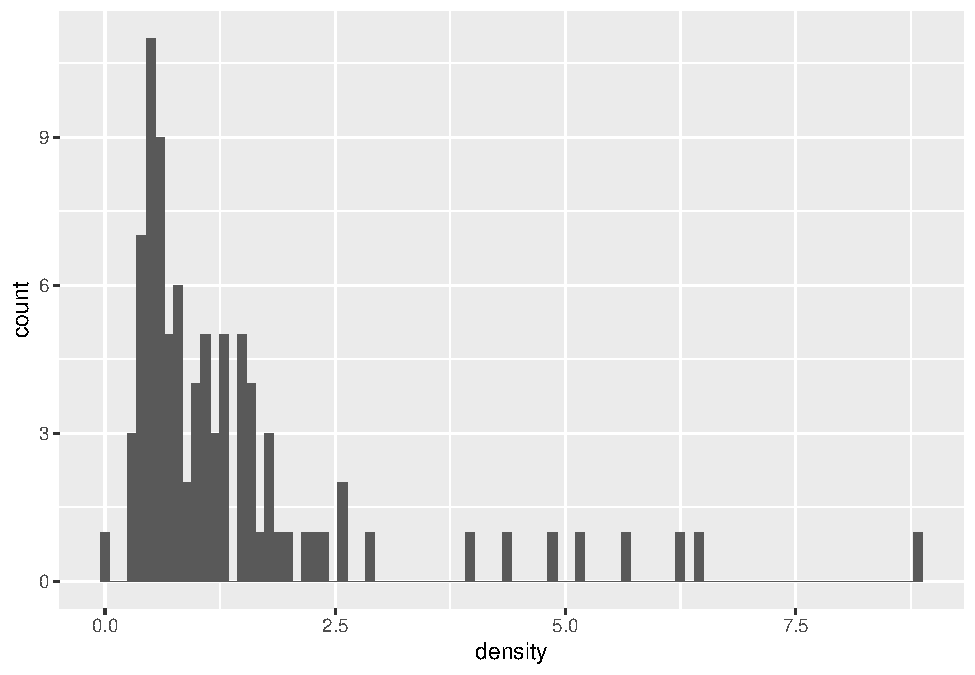
\includegraphics{Bagnard_Gaustad_Hartman_Leung_Lab_3_files/figure-latex/unnamed-chunk-37-1.pdf}

We note that one of the counties has an extremely low density. Near
zero.

\begin{Shaded}
\begin{Highlighting}[]
\NormalTok{dfCrime }\OperatorTok
\KeywordTok{filter}\NormalTok{(density }\OperatorTok{<}\StringTok{ }\FloatTok{0.01}\NormalTok{)}
\end{Highlighting}
\end{Shaded}

\begin{verbatim}
  county year    crmrte   prbarr  prbconv prbpris avgsen      polpc
1    173   87 0.0139937 0.530435 0.327869    0.15   6.64 0.00316379
      density    taxpc west central urban pctmin80    wcon     wtuc
1 2.03422e-05 37.72702    1       0     0 0.253914 231.696 213.6752
      wtrd    wfir     wser   wmfg   wfed   wsta   wloc       mix
1 175.1604 267.094 204.3792 193.01 334.44 414.68 304.32 0.4197531
     pctymle region regcode other nonurban         metro
1 0.07462687      1    West     0        1 Outside Metro
\end{verbatim}

In review of the North Carolina county density data from 1985, the
smallest population density in any county in North Carolina is 0.0952.
\url{http://ncosbm.s3.amazonaws.com/s3fs-public/demog/dens7095.xls}

This makes the density of 0.0000203422 for county 173 impossible. It is
miscoded and we will impute a new statistically predicted value.

\begin{Shaded}
\begin{Highlighting}[]
\NormalTok{dfCrime}\OperatorTok{$}\NormalTok{density[}\KeywordTok{which}\NormalTok{(dfCrime}\OperatorTok{$}\NormalTok{county}\OperatorTok{==}\DecValTok{173}\NormalTok{)]<-}\StringTok{ }\OtherTok{NA}
\end{Highlighting}
\end{Shaded}

\begin{Shaded}
\begin{Highlighting}[]
\NormalTok{impute_arg <-}\StringTok{ }\KeywordTok{aregImpute}\NormalTok{(}\OperatorTok{~}\StringTok{ }\NormalTok{crmrte }\OperatorTok{+}\StringTok{ }\NormalTok{urban }\OperatorTok{+}\StringTok{ }\NormalTok{central }\OperatorTok{+}\StringTok{ }\NormalTok{west }\OperatorTok{+}\StringTok{ }
\StringTok{                         }\NormalTok{prbarr }\OperatorTok{+}\StringTok{ }\NormalTok{prbconv }\OperatorTok{+}\StringTok{ }\NormalTok{prbpris }\OperatorTok{+}\StringTok{ }\NormalTok{avgsen }\OperatorTok{+}\StringTok{ }\NormalTok{polpc }\OperatorTok{+}
\StringTok{                         }\NormalTok{density }\OperatorTok{+}\StringTok{ }\NormalTok{taxpc }\OperatorTok{+}\StringTok{ }\NormalTok{pctmin80 }\OperatorTok{+}\StringTok{ }\NormalTok{wcon }\OperatorTok{+}\StringTok{ }\NormalTok{wtuc }\OperatorTok{+}
\StringTok{                         }\NormalTok{wtrd }\OperatorTok{+}\StringTok{ }\NormalTok{wfir }\OperatorTok{+}\StringTok{ }\NormalTok{wser }\OperatorTok{+}\StringTok{ }\NormalTok{wmfg }\OperatorTok{+}\StringTok{ }\NormalTok{wfed }\OperatorTok{+}\StringTok{ }\NormalTok{wsta }\OperatorTok{+}\StringTok{ }\NormalTok{wloc }\OperatorTok{+}
\StringTok{                         }\NormalTok{mix }\OperatorTok{+}\StringTok{ }\NormalTok{pctymle, }\DataTypeTok{data =}\NormalTok{ dfCrime, }\CommentTok{#%>% filter(urban==0 & west ==1),}
                         \DataTypeTok{match=}\StringTok{"weighted"}\NormalTok{,  }\DataTypeTok{nk=}\DecValTok{3}\NormalTok{, }\DataTypeTok{B=}\DecValTok{10}\NormalTok{, }\DataTypeTok{n.impute =} \DecValTok{100}\NormalTok{)}
\end{Highlighting}
\end{Shaded}

\begin{Shaded}
\begin{Highlighting}[]
\KeywordTok{paste}\NormalTok{(}\StringTok{"R-squares for Predicting Non-Missing Values for Each Variable"}\NormalTok{)}
\end{Highlighting}
\end{Shaded}

\begin{verbatim}
[1] "R-squares for Predicting Non-Missing Values for Each Variable"
\end{verbatim}

\begin{Shaded}
\begin{Highlighting}[]
\NormalTok{impute_arg}\OperatorTok{$}\NormalTok{rsq}
\end{Highlighting}
\end{Shaded}

\begin{verbatim}
  density 
0.9684228 
\end{verbatim}

\begin{Shaded}
\begin{Highlighting}[]
\KeywordTok{paste}\NormalTok{(}\StringTok{"Predicted values"}\NormalTok{)}
\end{Highlighting}
\end{Shaded}

\begin{verbatim}
[1] "Predicted values"
\end{verbatim}

\begin{Shaded}
\begin{Highlighting}[]
\KeywordTok{mean}\NormalTok{(impute_arg}\OperatorTok{$}\NormalTok{imputed}\OperatorTok{$}\NormalTok{density)}
\end{Highlighting}
\end{Shaded}

\begin{verbatim}
[1] 1.69431
\end{verbatim}

We will reassign this value using the mean from the trials.

\begin{Shaded}
\begin{Highlighting}[]
\NormalTok{dfCrime}\OperatorTok{$}\NormalTok{density[}\KeywordTok{which}\NormalTok{(dfCrime}\OperatorTok{$}\NormalTok{county}\OperatorTok{==}\DecValTok{173}\NormalTok{)]<-}\KeywordTok{mean}\NormalTok{(impute_arg}\OperatorTok{$}\NormalTok{imputed}\OperatorTok{$}\NormalTok{density)}
\end{Highlighting}
\end{Shaded}

With our variables transformed, we turn now to a discussion on
correlation in our data set. To facilitate our discussion we'll draw
reference to a network plot.

\begin{Shaded}
\begin{Highlighting}[]
\KeywordTok{options}\NormalTok{(}\DataTypeTok{repr.plot.width=}\DecValTok{6}\NormalTok{, }\DataTypeTok{repr.plot.height=}\DecValTok{6}\NormalTok{)}
\NormalTok{myData<-dfCrime}
\NormalTok{myData<-myData[, }\KeywordTok{c}\NormalTok{(}\StringTok{"crmrte"}\NormalTok{, }\StringTok{"west"}\NormalTok{, }\StringTok{"central"}\NormalTok{, }\StringTok{"other"}\NormalTok{, }\StringTok{"urban"}\NormalTok{, }\StringTok{"prbarr"}\NormalTok{, }\StringTok{"prbconv"}\NormalTok{, }\StringTok{"prbpris"}\NormalTok{, }\StringTok{"avgsen"}\NormalTok{, }\StringTok{"polpc"}\NormalTok{, }\StringTok{"taxpc"}\NormalTok{,}
           \StringTok{"pctmin80"}\NormalTok{, }\StringTok{"wcon"}\NormalTok{, }\StringTok{"wtuc"}\NormalTok{, }\StringTok{"wtrd"}\NormalTok{, }\StringTok{"wfir"}\NormalTok{, }\StringTok{"wser"}\NormalTok{, }\StringTok{"wmfg"}\NormalTok{, }\StringTok{"wfed"}\NormalTok{, }\StringTok{"wsta"}\NormalTok{, }\StringTok{"wloc"}\NormalTok{,}
           \StringTok{"mix"}\NormalTok{, }\StringTok{"pctymle"}\NormalTok{, }\StringTok{"density"}\NormalTok{)]}
\NormalTok{plot<-myData }\OperatorTok\StringTok{ }\KeywordTok{correlate}\NormalTok{() }\OperatorTok\StringTok{ }\KeywordTok{network_plot}\NormalTok{(}\DataTypeTok{min_cor=}\NormalTok{.}\DecValTok{2}\NormalTok{)}
\end{Highlighting}
\end{Shaded}

\begin{verbatim}

Correlation method: 'pearson'
Missing treated using: 'pairwise.complete.obs'
\end{verbatim}

\begin{Shaded}
\begin{Highlighting}[]
\KeywordTok{grid.arrange}\NormalTok{(}\KeywordTok{arrangeGrob}\NormalTok{(plot, }\DataTypeTok{bottom =} \StringTok{'Correlations Among Variables'}\NormalTok{),}
             \DataTypeTok{top =} \StringTok{"Network plot for Correlation Study"}\NormalTok{, }\DataTypeTok{ncol=}\DecValTok{1}\NormalTok{)}
\end{Highlighting}
\end{Shaded}

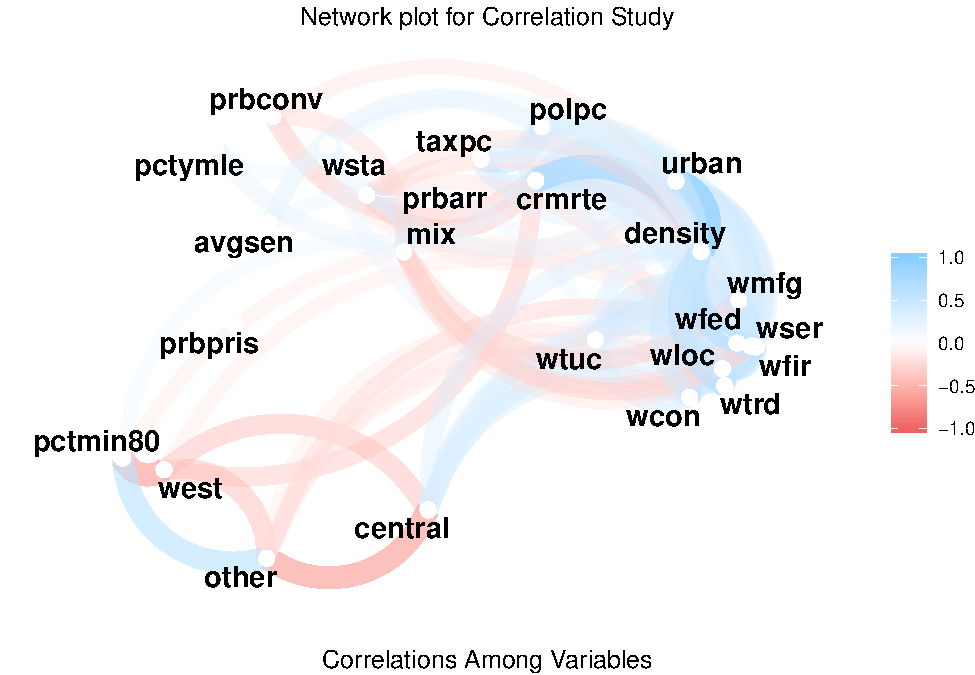
\includegraphics{Bagnard_Gaustad_Hartman_Leung_Lab_3_files/figure-latex/unnamed-chunk-43-1.pdf}
We first note in the network plot the general proximity of variables
with one another. Variables that are clustered together represent the
overall magnitude of their correlations. In fact, the cluster of the
wage variables are an indication of very tight correlation. Only state
wages fall outside this group. We also see the wage variables are
positively correlated with our crime outcome variable. Density also
positively correlates with wage and the crime rate variable. Urban
correlates with wage as well, but suprisingly the correlation between
crime and the urban indicator variable is not as high, leading us to
suspect that density may tell a better story.

Next, we notice the Law enforcement and Judicial variables are clustered
together and have a negative correlation with our outcome variable on
crime. We also see they tend to be negatively correlated amongst one
another. For example, probability of conviction is slightly negatively
corrrelated with the probability of arrest, and both are negatively
correlated with our outcome variable. We also see that police per capita
and tax per capita are positively correlated with another. This makes
sense as the more revenues collected the higher the ability to pay for
law enforcement and protection services. Both are also positively
correlated with our outcome variable on crime. We also notice that
percent young male has a positive correlation with crime rate. A
possible explanation for this is that more crimes are committed by
younger men as a whole.

The mix variable is an odd one. It possitively correlates with
probability of arrests, negatively correlates with probability of
convictions, and negatively correlates with service and manufacturing
wages. It also has a slight positive correlation with the state wage
variable and seems to be clustered with it.

Last, we turn to our region variables and notice the high negative
correlation of the minority variable with the western region variable.
We also notice a high positive corrlation of minorities with the `other'
(coastal) variable. The pctmin80 variable also correlates positively
with crime rate, although the two are not clustered. We especially note
that west is negatively correlated with crime rate. There appears to be
a lessor propensity for crime in this region, or perhaps a lack of
suffient means to detect it. We put this knowledge in our back pocket.

A note to the interested party - for a futher examination of network
plots describing correlations in each of the regions please see the
diagrams in our appendix. If you are curious about the relationships of
data between groups we think you will enjoy them.

\hypertarget{summary-and-results}{%
\subsection{Summary and Results}\label{summary-and-results}}

Our outcome variable is the \emph{crime rate} (``crmrte'') variable,
which is defined as the crimes committed per person in a specific county
during 1987. The crime rate of the 90 counties in our sample dataset
range between 0.0055 - 0.0990, with a mean of 0.0335.

From the boxplot below, most of the counties have a crime rate between
0.0055 and 0.0700, with 5 outliers having a crime rate \textgreater{}
0.0700.

\begin{Shaded}
\begin{Highlighting}[]
\KeywordTok{options}\NormalTok{(}\DataTypeTok{repr.plot.width=}\DecValTok{8}\NormalTok{, }\DataTypeTok{repr.plot.height=}\DecValTok{4}\NormalTok{)}
\NormalTok{p<-}\KeywordTok{ggplot}\NormalTok{(}\DataTypeTok{data =}\NormalTok{ dfCrime, }\KeywordTok{aes}\NormalTok{(}\DataTypeTok{y =}\NormalTok{ crmrte, }\DataTypeTok{color =}\NormalTok{ regcode)) }\OperatorTok{+}
\StringTok{     }\KeywordTok{geom_boxplot}\NormalTok{(}\DataTypeTok{show.legend=}\OtherTok{FALSE}\NormalTok{) }\OperatorTok{+}\StringTok{ }\KeywordTok{facet_wrap}\NormalTok{(}\OperatorTok{~}\StringTok{ }\NormalTok{regcode)}
\NormalTok{p2<-}\KeywordTok{ggplot}\NormalTok{(}\DataTypeTok{data =}\NormalTok{ dfCrime, }\KeywordTok{aes}\NormalTok{(}\DataTypeTok{y =}\NormalTok{ crmrte)) }\OperatorTok{+}
\StringTok{     }\KeywordTok{geom_boxplot}\NormalTok{()}
\KeywordTok{grid.arrange}\NormalTok{(p, p2, }\DataTypeTok{ncol=}\DecValTok{2}\NormalTok{)}
\end{Highlighting}
\end{Shaded}

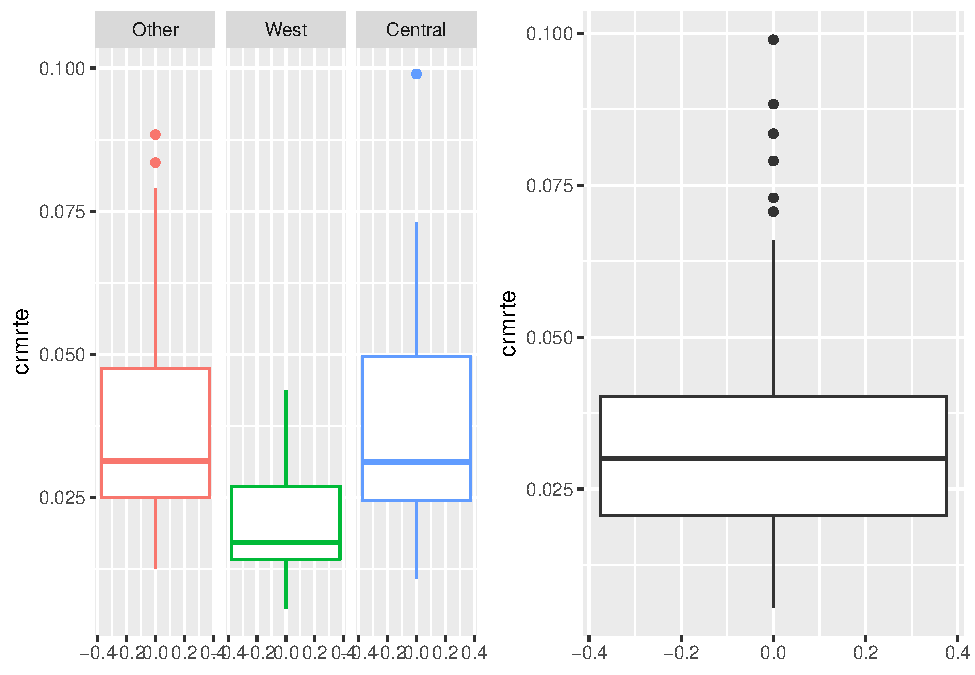
\includegraphics{Bagnard_Gaustad_Hartman_Leung_Lab_3_files/figure-latex/unnamed-chunk-44-1.pdf}

Extending the discussion of mix from our initial correllation
discussion, we further note that mix is defined as the type of crime
committed. Our research focuses on providing policy recommendations to
reduce crime in general, and not a specific type of crime. As a result
we will not include additional focus on this variable.

We propose 3 multiple linear regression models

\begin{itemize}
\item
  First Model: Has basic explanatory variables of key interest by
  region, and no other covariates.
\item
  Second Model: Includes the explanatory variables and covariates that
  increase the accuracy of our results without substantial bias.
\item
  Third Model: An expansion of the second model with most covariates,
  designed to demonstrate the robustness of our results before yielding
  to a discussion on observations of our model specifications.
\end{itemize}

\hypertarget{model-analysis}{%
\section{Model Analysis}\label{model-analysis}}

\hypertarget{model-1}{%
\subsection{Model 1}\label{model-1}}

\hypertarget{introduction-1}{%
\subsubsection{Introduction}\label{introduction-1}}

Our base hypothesis is that county level crime can be fundamentally
explained by three factors in a county: the effectiveness of the
criminal justice system, economic conditions, and regional variations.

\begin{itemize}
\tightlist
\item
  \textbf{Criminal Justice Effectiveness}\\
  Criminal Justice Effectiveness is an abstract concept that is
  operationalized by comparing the number of crimes to convictions. To
  track crimes, they must be reported to police, who can then make
  arrests. Then, the legal system provides judgement in the form of
  convictions and sentencing. Besides removing some criminals from
  society, criminal justice can serve as deterrent, as the probability
  of getting caught, convicted, and sentenced could discourage some
  would-be criminals from committing crimes.
\end{itemize}

\begin{quote}
We operationalize criminal justice effectiveness as (probability of
Convictions for Crimes committed). We define this as: prbconv * prbarr =
conv/arrest * arrest/crime = convictions/crime. Without more granular
data, this provides a single parsimonious metric that helps understand
how well the law enforcement and criminal justice system works.
\end{quote}

\begin{Shaded}
\begin{Highlighting}[]
\NormalTok{dfCrime}\OperatorTok{$}\NormalTok{crimJustEff<-dfCrime}\OperatorTok{$}\NormalTok{prbarr }\OperatorTok{*}\StringTok{ }\NormalTok{dfCrime}\OperatorTok{$}\NormalTok{prbconv}
\end{Highlighting}
\end{Shaded}

\begin{itemize}
\item
  \textbf{Region}\\
  Region is easily identified as possible factor for predicting crime as
  seen from our initial EDA in the Introduction. It would be expected
  that cultural, economic, government, geographic, and demographic
  profiles among other important variables would vary across the
  regions. Without the ability to measure and operationalize these
  variables, region offers us a suitable proxy for stand in.
\item
  \textbf{Economic Conditions}\\
  Finally, we theorize that the third major cause of crime is economic
  conditions. We would expect that as someone's economic success and
  opportunity increases, their propensity to commit crime is lowered.
  And similarly when there are worse economic conditions, crime would
  increase due to lack of means, lack of occupation or boredom. This
  also means that individuals have less to look forward to and are
  willing to risk their freedom or endanger themselves.
\end{itemize}

\begin{quote}
We operationalize economic conditions by looking at wages, which
includes the sum of all average weekly wages from the 1980 census
information in our data set. For this base, parsimonious model, we
define economic opportunity as the \emph{scaled} average weekly pay from
each sector provided in the data set. We scale this variable by dividing
the sum by 9 to keep the magnitude matched to the original variables.
Ideally, we would like to use a weighted average, but given the lack of
data, we think this is best proxy from our data because it answers all
of the above (higher wages leads to better means and better
opportunities). From our EDA we also confirm that in general these sums
are not skewed by having one really high paying sector in each county as
we see a strong relationship between average quartile across all job
types and sector average wages.
\end{quote}

\begin{Shaded}
\begin{Highlighting}[]
\NormalTok{dfCrime}\OperatorTok{$}\NormalTok{scaledWages<-(dfCrime}\OperatorTok{$}\NormalTok{wcon }\OperatorTok{+}\StringTok{ }\NormalTok{dfCrime}\OperatorTok{$}\NormalTok{wtuc }\OperatorTok{+}\StringTok{ }\NormalTok{dfCrime}\OperatorTok{$}\NormalTok{wtrd }\OperatorTok{+}\StringTok{ }\NormalTok{dfCrime}\OperatorTok{$}\NormalTok{wfir }\OperatorTok{+}
\StringTok{    }\NormalTok{dfCrime}\OperatorTok{$}\NormalTok{wser }\OperatorTok{+}\StringTok{ }\NormalTok{dfCrime}\OperatorTok{$}\NormalTok{wmfg }\OperatorTok{+}\StringTok{ }\NormalTok{dfCrime}\OperatorTok{$}\NormalTok{wfed }\OperatorTok{+}\StringTok{ }\NormalTok{dfCrime}\OperatorTok{$}\NormalTok{wsta }\OperatorTok{+}\StringTok{ }\NormalTok{dfCrime}\OperatorTok{$}\NormalTok{wloc) }\OperatorTok{/}\StringTok{ }\DecValTok{9}
\end{Highlighting}
\end{Shaded}

\hypertarget{model-1-eda}{%
\subsubsection{Model 1 EDA}\label{model-1-eda}}

\textbf{Data Transformations: Criminal Justice Effectiveness}\\
First we look at the components of the Criminal Justice Effectiveness:
Probability of arrest and Probability of conviction.

\begin{Shaded}
\begin{Highlighting}[]
\NormalTok{p1 <-}\StringTok{ }\KeywordTok{ggplot}\NormalTok{(dfCrime, }\KeywordTok{aes}\NormalTok{(}\DataTypeTok{x =}\NormalTok{ prbarr, }\DataTypeTok{color=}\NormalTok{regcode, }\DataTypeTok{fill =}\NormalTok{ regcode)) }\OperatorTok{+}
\StringTok{  }\KeywordTok{geom_histogram}\NormalTok{(}\DataTypeTok{position=}\StringTok{"identity"}\NormalTok{, }\DataTypeTok{alpha=}\FloatTok{0.5}\NormalTok{, }\DataTypeTok{bins=}\DecValTok{30}\NormalTok{) }\OperatorTok{+}
\StringTok{  }\KeywordTok{labs}\NormalTok{(}\DataTypeTok{title=}\StringTok{"Probability of Arrest"}\NormalTok{, }\DataTypeTok{x=}\StringTok{"Arrest per Crime"}\NormalTok{, }\DataTypeTok{y=}\StringTok{"Count"}\NormalTok{)}
\NormalTok{p2 <-}\StringTok{ }\KeywordTok{ggplot}\NormalTok{(dfCrime, }\KeywordTok{aes}\NormalTok{(}\DataTypeTok{x =}\NormalTok{ prbconv, }\DataTypeTok{color=}\NormalTok{regcode, }\DataTypeTok{fill =}\NormalTok{ regcode)) }\OperatorTok{+}
\StringTok{  }\KeywordTok{geom_histogram}\NormalTok{(}\DataTypeTok{position=}\StringTok{"identity"}\NormalTok{, }\DataTypeTok{alpha=}\FloatTok{0.5}\NormalTok{, }\DataTypeTok{bins=}\DecValTok{30}\NormalTok{) }\OperatorTok{+}
\StringTok{  }\KeywordTok{labs}\NormalTok{(}\DataTypeTok{title=}\StringTok{"Probability of Conviction"}\NormalTok{, }\DataTypeTok{x=}\StringTok{"Conviction per Arrest"}\NormalTok{, }\DataTypeTok{y=}\StringTok{"Count"}\NormalTok{)}
\KeywordTok{grid.arrange}\NormalTok{(p2, p1, }\DataTypeTok{ncol=}\DecValTok{2}\NormalTok{)}
\end{Highlighting}
\end{Shaded}

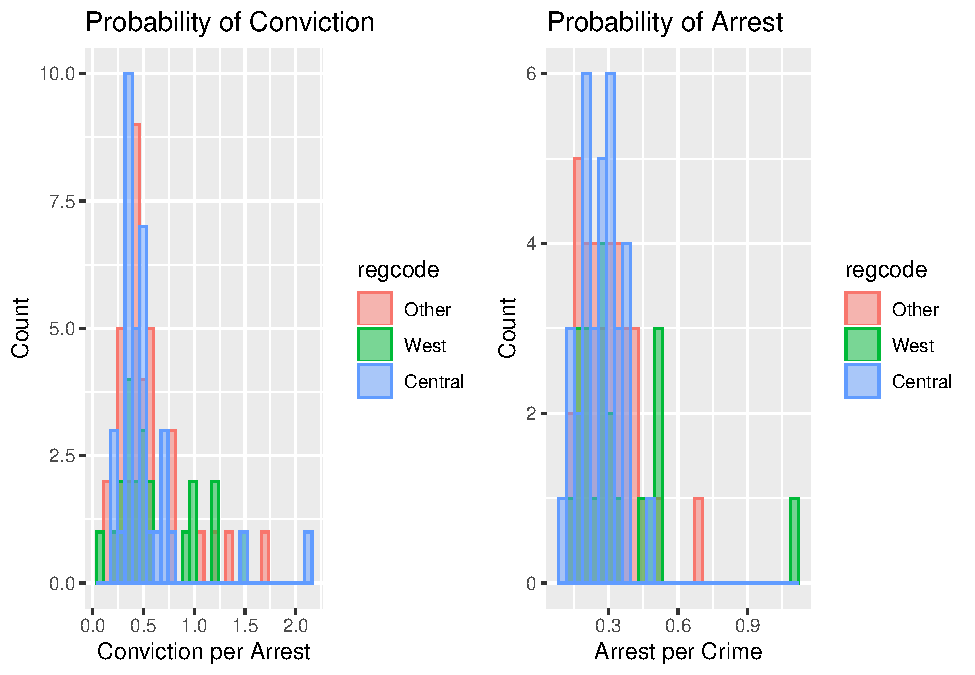
\includegraphics{Bagnard_Gaustad_Hartman_Leung_Lab_3_files/figure-latex/unnamed-chunk-47-1.pdf}

The distribution of both probability of conviction and probability of
arrest are skewed right. It could be argued that both of these variables
should be bound between 0 and 1. However, these ``probabilities'' are
proxied by ratios. It is in fact possible (and perhaps common) that
defendants are charged with multiple crimes and convicted, but were only
arrested once. For this reason we will not consider outliers in this
variable.

For ``probability'' of arrest, it could also be possible there are
multiple arrests for a single crime. However, we have one single data
point greater than one, and it is \textgreater{}5 standard deviations
away from the distribution. Since this value falls so far out of
distribution, it will have high leverage on our model. We will
preemptively impute its value as the current data point is likely an
error, and is not representative of the bulk of North Carolina counties.

\begin{Shaded}
\begin{Highlighting}[]
\CommentTok{# County number of outlier}
\NormalTok{(dfCrime}\OperatorTok{$}\NormalTok{county[dfCrime}\OperatorTok{$}\NormalTok{crimJustEff }\OperatorTok{>}\StringTok{ }\DecValTok{1}\NormalTok{]) }
\end{Highlighting}
\end{Shaded}

\begin{verbatim}
[1] 115
90 Levels: 1 3 5 7 9 11 13 15 17 19 21 23 25 27 33 35 37 39 41 45 ... 197
\end{verbatim}

\begin{Shaded}
\begin{Highlighting}[]
\CommentTok{# how many standard deviations away the outlier lies}
\NormalTok{(dfCrime[dfCrime}\OperatorTok{$}\NormalTok{crimJustEff }\OperatorTok{>}\StringTok{ }\DecValTok{1}\NormalTok{,]}\OperatorTok{$}\NormalTok{prbarr }\OperatorTok{-}\StringTok{ }\KeywordTok{mean}\NormalTok{(dfCrime}\OperatorTok{$}\NormalTok{prbarr))}\OperatorTok{/}\KeywordTok{sd}\NormalTok{(dfCrime}\OperatorTok{$}\NormalTok{prbarr)}
\end{Highlighting}
\end{Shaded}

\begin{verbatim}
[1] 5.779438
\end{verbatim}

We will use the imputation method to replace the large prbarr value and
remove the outlier effect, while also retaining the rest of the
information about the county.

\begin{Shaded}
\begin{Highlighting}[]
\NormalTok{dfCrime}\OperatorTok{$}\NormalTok{prbarr[}\KeywordTok{which}\NormalTok{(dfCrime}\OperatorTok{$}\NormalTok{county}\OperatorTok{==}\DecValTok{115}\NormalTok{)]<-}\OtherTok{NA} \CommentTok{# set the value to NA so it will be imputed}
\end{Highlighting}
\end{Shaded}

\begin{Shaded}
\begin{Highlighting}[]
\NormalTok{impute_arg <-}\StringTok{ }\KeywordTok{aregImpute}\NormalTok{(}\OperatorTok{~}\StringTok{ }\NormalTok{crmrte }\OperatorTok{+}\StringTok{  }\NormalTok{urban }\OperatorTok{+}\StringTok{ }\NormalTok{central }\OperatorTok{+}\StringTok{ }\NormalTok{west }\OperatorTok{+}\StringTok{ }\NormalTok{other }\OperatorTok{+}
\StringTok{                         }\NormalTok{prbarr }\OperatorTok{+}\StringTok{ }\NormalTok{prbconv }\OperatorTok{+}\StringTok{ }\NormalTok{prbpris }\OperatorTok{+}\StringTok{ }\NormalTok{avgsen }\OperatorTok{+}\StringTok{ }\NormalTok{polpc }\OperatorTok{+}
\StringTok{                         }\NormalTok{density }\OperatorTok{+}\StringTok{ }\NormalTok{taxpc }\OperatorTok{+}\StringTok{ }\NormalTok{pctmin80 }\OperatorTok{+}\StringTok{ }\NormalTok{wcon }\OperatorTok{+}\StringTok{ }\NormalTok{wtuc }\OperatorTok{+}
\StringTok{                         }\NormalTok{wtrd }\OperatorTok{+}\StringTok{ }\NormalTok{wfir }\OperatorTok{+}\StringTok{ }\NormalTok{wser }\OperatorTok{+}\StringTok{ }\NormalTok{wmfg }\OperatorTok{+}\StringTok{ }\NormalTok{wfed }\OperatorTok{+}\StringTok{ }\NormalTok{wsta }\OperatorTok{+}\StringTok{ }\NormalTok{wloc }\OperatorTok{+}
\StringTok{                         }\NormalTok{mix }\OperatorTok{+}\StringTok{ }\NormalTok{pctymle, }\DataTypeTok{data =}\NormalTok{ dfCrime, }\DataTypeTok{match=}\StringTok{"weighted"}\NormalTok{,}
                         \DataTypeTok{nk=}\DecValTok{3}\NormalTok{, }\DataTypeTok{B=}\DecValTok{10}\NormalTok{, }\DataTypeTok{n.impute =} \DecValTok{100}\NormalTok{)}
\end{Highlighting}
\end{Shaded}

\begin{Shaded}
\begin{Highlighting}[]
\KeywordTok{paste}\NormalTok{(}\StringTok{"R-squares for Predicting Non-Missing Values for Each Variable"}\NormalTok{)}
\end{Highlighting}
\end{Shaded}

\begin{verbatim}
[1] "R-squares for Predicting Non-Missing Values for Each Variable"
\end{verbatim}

\begin{Shaded}
\begin{Highlighting}[]
\NormalTok{impute_arg}\OperatorTok{$}\NormalTok{rsq}
\end{Highlighting}
\end{Shaded}

\begin{verbatim}
   prbarr 
0.8854613 
\end{verbatim}

\begin{Shaded}
\begin{Highlighting}[]
\KeywordTok{paste}\NormalTok{(}\StringTok{"Predicted values"}\NormalTok{)}
\end{Highlighting}
\end{Shaded}

\begin{verbatim}
[1] "Predicted values"
\end{verbatim}

\begin{Shaded}
\begin{Highlighting}[]
\KeywordTok{mean}\NormalTok{(impute_arg}\OperatorTok{$}\NormalTok{imputed}\OperatorTok{$}\NormalTok{prbarr)}
\end{Highlighting}
\end{Shaded}

\begin{verbatim}
[1] 0.3317323
\end{verbatim}

We will reassign this value using the mean from the trials.

\begin{Shaded}
\begin{Highlighting}[]
\NormalTok{dfCrime}\OperatorTok{$}\NormalTok{prbarr[}\KeywordTok{which}\NormalTok{(dfCrime}\OperatorTok{$}\NormalTok{county}\OperatorTok{==}\DecValTok{115}\NormalTok{)]<-}\KeywordTok{mean}\NormalTok{(impute_arg}\OperatorTok{$}\NormalTok{imputed}\OperatorTok{$}\NormalTok{prbarr)}
\end{Highlighting}
\end{Shaded}

With the outlier imputed, the Criminal Justice Effectiveness can be
constructed. We present a histogram showing how log transformation can
also improve normality. Be conducting a log transformation we can also
understand the resulting coefficient as a percent change in the ratio of
Criminal Justice Effectiveness (convictions/crime) which will be more
helpful in communicating recommendations for policy.

\begin{Shaded}
\begin{Highlighting}[]
\NormalTok{dfCrime}\OperatorTok{$}\NormalTok{crimJustEff<-dfCrime}\OperatorTok{$}\NormalTok{prbarr }\OperatorTok{*}\StringTok{ }\NormalTok{dfCrime}\OperatorTok{$}\NormalTok{prbconv}
\NormalTok{dfCrime}\OperatorTok{$}\NormalTok{logcrimJustEff<-}\KeywordTok{log}\NormalTok{(dfCrime}\OperatorTok{$}\NormalTok{crimJustEff)}
\NormalTok{dfCrime}\OperatorTok{$}\NormalTok{logcrmrte <-}\StringTok{ }\KeywordTok{log}\NormalTok{(dfCrime}\OperatorTok{$}\NormalTok{crmrte)}
\KeywordTok{options}\NormalTok{(}\DataTypeTok{repr.plot.width=}\DecValTok{4}\NormalTok{, }\DataTypeTok{repr.plot.height=}\DecValTok{4}\NormalTok{)}
\NormalTok{p1 <-}\StringTok{ }\KeywordTok{ggplot}\NormalTok{(dfCrime, }\KeywordTok{aes}\NormalTok{(}\DataTypeTok{x =}\NormalTok{ crimJustEff, }\DataTypeTok{color=}\NormalTok{regcode, }\DataTypeTok{fill =}\NormalTok{ regcode)) }\OperatorTok{+}
\StringTok{  }\KeywordTok{geom_histogram}\NormalTok{(}\DataTypeTok{position=}\StringTok{"identity"}\NormalTok{, }\DataTypeTok{alpha=}\FloatTok{0.5}\NormalTok{, }\DataTypeTok{bins=}\DecValTok{30}\NormalTok{) }\OperatorTok{+}
\StringTok{  }\KeywordTok{labs}\NormalTok{(}\DataTypeTok{title=}\StringTok{"Criminal Justice Effectiveness"}\NormalTok{, }\DataTypeTok{x=}\StringTok{"Convictions per Crime"}\NormalTok{, }\DataTypeTok{y=}\StringTok{"Count"}\NormalTok{)}
\NormalTok{p2 <-}\StringTok{ }\KeywordTok{ggplot}\NormalTok{(dfCrime, }\KeywordTok{aes}\NormalTok{(}\DataTypeTok{x =}\NormalTok{ logcrimJustEff, }\DataTypeTok{color=}\NormalTok{regcode, }\DataTypeTok{fill =}\NormalTok{ regcode)) }\OperatorTok{+}
\StringTok{  }\KeywordTok{geom_histogram}\NormalTok{(}\DataTypeTok{position=}\StringTok{"identity"}\NormalTok{, }\DataTypeTok{alpha=}\FloatTok{0.5}\NormalTok{, }\DataTypeTok{bins=}\DecValTok{30}\NormalTok{) }\OperatorTok{+}
\StringTok{  }\KeywordTok{labs}\NormalTok{(}\DataTypeTok{title=}\StringTok{"log(Criminal Justice Effectiveness)"}\NormalTok{, }\DataTypeTok{x=}\StringTok{"log(Convictions per Crime)"}\NormalTok{, }\DataTypeTok{y=}\StringTok{"Count"}\NormalTok{)}
\KeywordTok{grid.arrange}\NormalTok{(p1, p2, }\DataTypeTok{ncol=}\DecValTok{2}\NormalTok{)}
\end{Highlighting}
\end{Shaded}

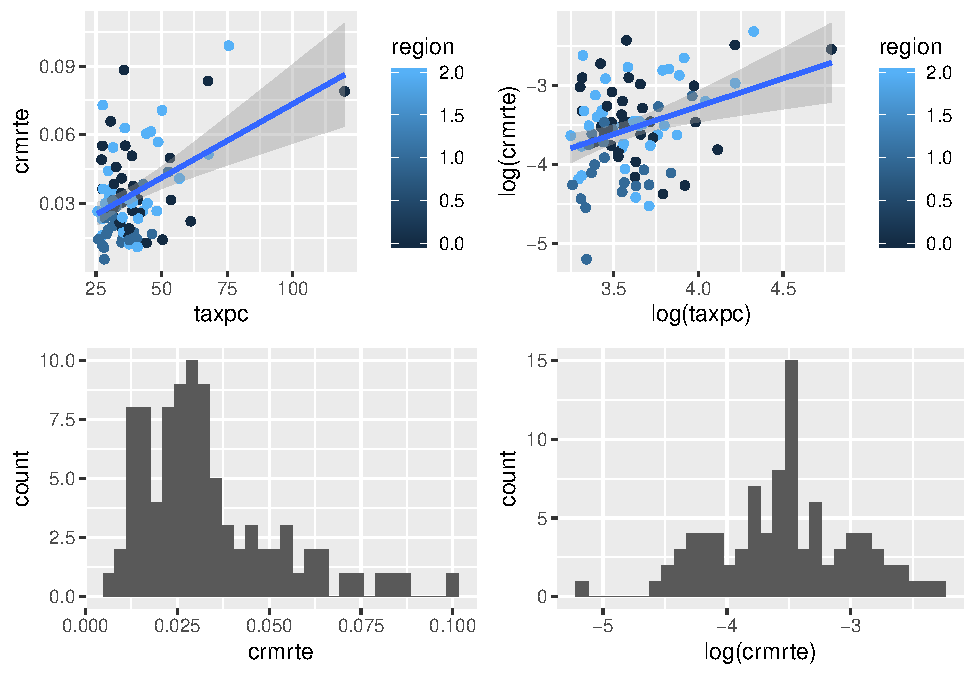
\includegraphics{Bagnard_Gaustad_Hartman_Leung_Lab_3_files/figure-latex/unnamed-chunk-53-1.pdf}

\textbf{Data Transformations: Unweighted Average of Sector Wages}

We turn our attention now to the economic variable, the scaled average
wage of all provided sectors. The wages trend together well, so there is
limited information lost when combining them into one variable. This can
be seen by plotting quartiles of each wage against the scaled average
and observing a relatively linear response.

\begin{Shaded}
\begin{Highlighting}[]
\CommentTok{# # Quantiles for all jobs}
\NormalTok{dfWage<-}\KeywordTok{mutate}\NormalTok{(dfCrime,}\DataTypeTok{qCon=}\KeywordTok{ntile}\NormalTok{(dfCrime}\OperatorTok{$}\NormalTok{wcon,}\DecValTok{4}\NormalTok{))}
\NormalTok{dfWage<-}\KeywordTok{mutate}\NormalTok{(dfWage,}\DataTypeTok{qTuc=}\KeywordTok{ntile}\NormalTok{(dfCrime}\OperatorTok{$}\NormalTok{wtuc,}\DecValTok{4}\NormalTok{))}
\NormalTok{dfWage<-}\KeywordTok{mutate}\NormalTok{(dfWage,}\DataTypeTok{qTrd=}\KeywordTok{ntile}\NormalTok{(dfCrime}\OperatorTok{$}\NormalTok{wtrd,}\DecValTok{4}\NormalTok{))}
\NormalTok{dfWage<-}\KeywordTok{mutate}\NormalTok{(dfWage,}\DataTypeTok{qFir=}\KeywordTok{ntile}\NormalTok{(dfCrime}\OperatorTok{$}\NormalTok{wfir,}\DecValTok{4}\NormalTok{))}
\NormalTok{dfWage<-}\KeywordTok{mutate}\NormalTok{(dfWage,}\DataTypeTok{qSer=}\KeywordTok{ntile}\NormalTok{(dfCrime}\OperatorTok{$}\NormalTok{wser,}\DecValTok{4}\NormalTok{))}
\NormalTok{dfWage<-}\KeywordTok{mutate}\NormalTok{(dfWage,}\DataTypeTok{qMfg=}\KeywordTok{ntile}\NormalTok{(dfCrime}\OperatorTok{$}\NormalTok{wmfg,}\DecValTok{4}\NormalTok{))}
\NormalTok{dfWage<-}\KeywordTok{mutate}\NormalTok{(dfWage,}\DataTypeTok{qFed=}\KeywordTok{ntile}\NormalTok{(dfCrime}\OperatorTok{$}\NormalTok{wfed,}\DecValTok{4}\NormalTok{))}
\NormalTok{dfWage<-}\KeywordTok{mutate}\NormalTok{(dfWage,}\DataTypeTok{qSta=}\KeywordTok{ntile}\NormalTok{(dfCrime}\OperatorTok{$}\NormalTok{wsta,}\DecValTok{4}\NormalTok{))}
\NormalTok{dfWage<-}\KeywordTok{mutate}\NormalTok{(dfWage,}\DataTypeTok{qLoc=}\KeywordTok{ntile}\NormalTok{(dfCrime}\OperatorTok{$}\NormalTok{wloc,}\DecValTok{4}\NormalTok{))}
\CommentTok{## Average quantile}
\NormalTok{dfWage}\OperatorTok{$}\NormalTok{qAvg=}\StringTok{ }\NormalTok{(dfWage}\OperatorTok{$}\NormalTok{qCon}\OperatorTok{+}\NormalTok{dfWage}\OperatorTok{$}\NormalTok{qTuc}\OperatorTok{+}\NormalTok{dfWage}\OperatorTok{$}\NormalTok{qTrd}\OperatorTok{+}\NormalTok{dfWage}\OperatorTok{$}\NormalTok{qFir}\OperatorTok{+}\NormalTok{dfWage}\OperatorTok{$}\NormalTok{qSer}\OperatorTok{+}\NormalTok{dfWage}\OperatorTok{$}\NormalTok{qMfg}\OperatorTok{+}
\StringTok{                }\NormalTok{dfWage}\OperatorTok{$}\NormalTok{qFed}\OperatorTok{+}\NormalTok{dfWage}\OperatorTok{$}\NormalTok{qSta}\OperatorTok{+}\NormalTok{dfWage}\OperatorTok{$}\NormalTok{qLoc)}\OperatorTok{/}\DecValTok{9}

\KeywordTok{plot}\NormalTok{(dfCrime}\OperatorTok{$}\NormalTok{scaledWages,dfWage}\OperatorTok{$}\NormalTok{qAvg)}
\end{Highlighting}
\end{Shaded}

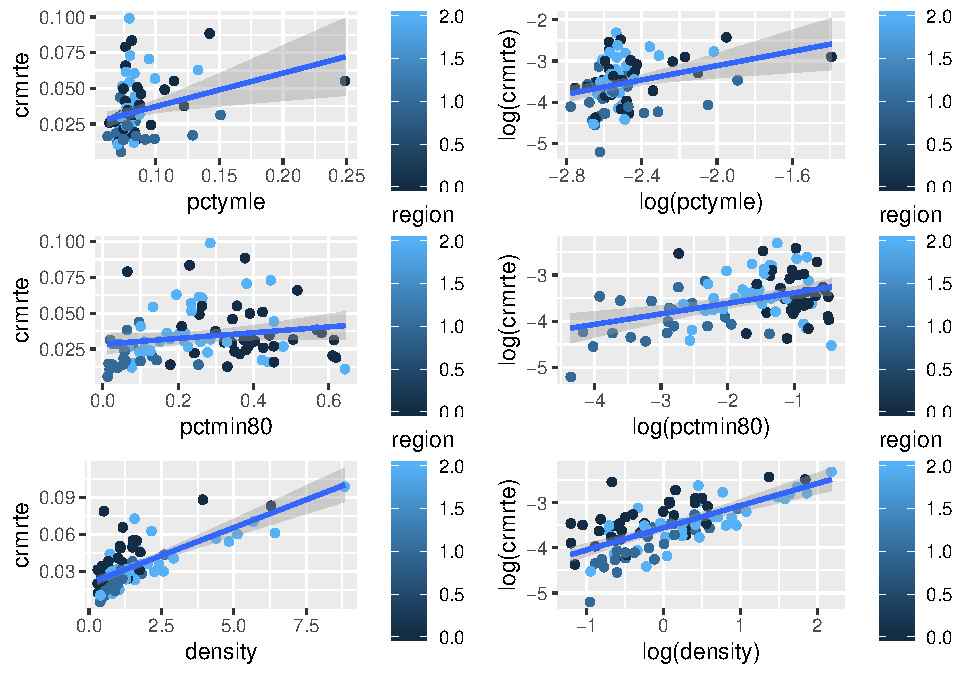
\includegraphics{Bagnard_Gaustad_Hartman_Leung_Lab_3_files/figure-latex/unnamed-chunk-54-1.pdf}

We again modify this variable with a log transformation for better
interpretation. This allows us to interpret percent changes in wage
which is more consistent across a range of wages. The result is a
relatively normal distribution as seen in the below histogram. We note
that there is a small ``second mode'' for the Central region, but this
is not very concerning.

\begin{Shaded}
\begin{Highlighting}[]
\NormalTok{dfCrime}\OperatorTok{$}\NormalTok{logScaledWages <-}\StringTok{ }\KeywordTok{log}\NormalTok{(dfCrime}\OperatorTok{$}\NormalTok{scaledWages)}
\NormalTok{p1 <-}\StringTok{ }\KeywordTok{ggplot}\NormalTok{(dfCrime, }\KeywordTok{aes}\NormalTok{(}\DataTypeTok{x =}\NormalTok{ logScaledWages, }\DataTypeTok{color=}\NormalTok{regcode, }\DataTypeTok{fill =}\NormalTok{ regcode)) }\OperatorTok{+}
\StringTok{  }\KeywordTok{geom_histogram}\NormalTok{(}\DataTypeTok{position=}\StringTok{"identity"}\NormalTok{, }\DataTypeTok{alpha=}\FloatTok{0.5}\NormalTok{, }\DataTypeTok{bins=}\DecValTok{30}\NormalTok{) }\OperatorTok{+}
\StringTok{  }\KeywordTok{labs}\NormalTok{(}\DataTypeTok{title=}\StringTok{"log(Scaled Wages)"}\NormalTok{, }\DataTypeTok{x=}\StringTok{"log(Scaled Wages)"}\NormalTok{, }\DataTypeTok{y=}\StringTok{"Count"}\NormalTok{)}
\NormalTok{p1}
\end{Highlighting}
\end{Shaded}

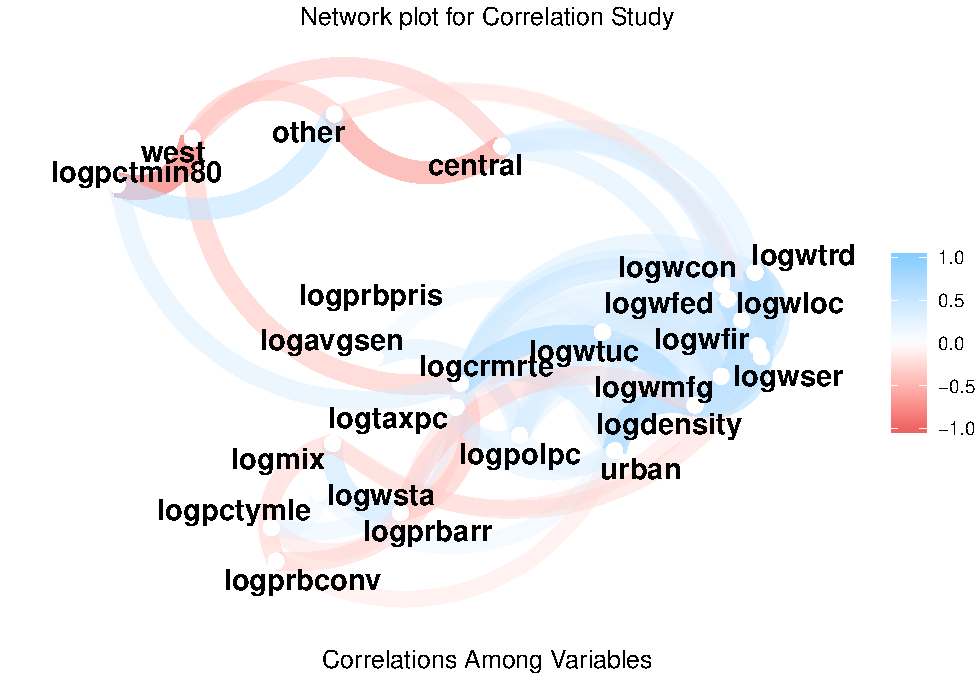
\includegraphics{Bagnard_Gaustad_Hartman_Leung_Lab_3_files/figure-latex/unnamed-chunk-55-1.pdf}
Interestingly, when viewing the wage data plotted against crime rate
(below) we see that there is a positive correlation between wages and
crime. In model 1, we will see if this holds true when taking into
account the effect of Criminal Justice Effectiveness and discuss some
possible causes.

\begin{Shaded}
\begin{Highlighting}[]
\NormalTok{q9<-}\KeywordTok{ggplot}\NormalTok{(}\DataTypeTok{data =}\NormalTok{ dfCrime, }\KeywordTok{aes}\NormalTok{(}\DataTypeTok{x =}\NormalTok{ logScaledWages, }\DataTypeTok{y =}\NormalTok{ logcrmrte, }\DataTypeTok{color =}\NormalTok{ regcode)) }\OperatorTok{+}
\StringTok{      }\KeywordTok{geom_point}\NormalTok{()}\OperatorTok{+}
\StringTok{  }\KeywordTok{geom_smooth}\NormalTok{(}\DataTypeTok{method =} \StringTok{"lm"}\NormalTok{)}
\KeywordTok{options}\NormalTok{(}\DataTypeTok{repr.plot.width=}\DecValTok{8}\NormalTok{, }\DataTypeTok{repr.plot.height=}\DecValTok{16}\NormalTok{)}
\NormalTok{q9}
\end{Highlighting}
\end{Shaded}

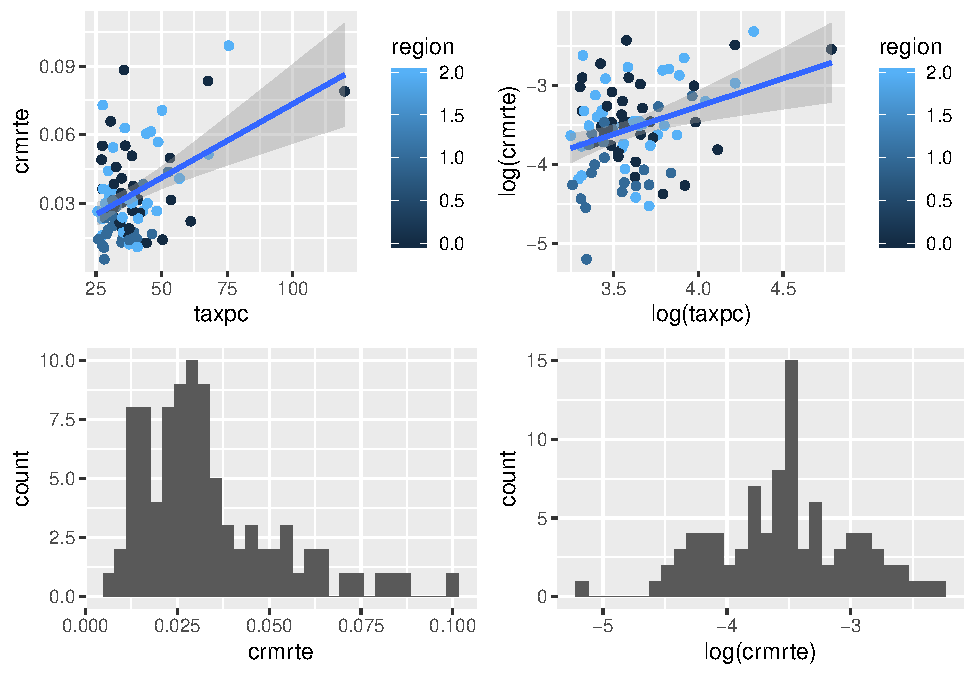
\includegraphics{Bagnard_Gaustad_Hartman_Leung_Lab_3_files/figure-latex/unnamed-chunk-56-1.pdf}

\textbf{Data Transformations: Crime Rate}\\
Our dependent variable is crime. Operationalized it is given as a rate
of crimes per capita. We will apply a log transform for two reasons.
First, since this value tends to be small (\textless{}.1), the log
transform gives us a much better range away from zero, and limits the
effect of high crime counties from exerting large leverage on our model.
Second, the log transform allows us talk about relative percentage
changes in crime rate for the counties. This allows changes in crime
rate to be reported in percent which is relevant to all counties,
irrespective of their current status as low or high crime counties. In
the below histograms, the improved normality is also observed in the log
transformed variable.

\begin{Shaded}
\begin{Highlighting}[]
\NormalTok{dfCrime}\OperatorTok{$}\NormalTok{logcrmrte <-}\StringTok{ }\KeywordTok{log}\NormalTok{(dfCrime}\OperatorTok{$}\NormalTok{crmrte)}
\KeywordTok{options}\NormalTok{(}\DataTypeTok{repr.plot.width=}\DecValTok{4}\NormalTok{, }\DataTypeTok{repr.plot.height=}\DecValTok{4}\NormalTok{)}
\NormalTok{p1 <-}\StringTok{ }\KeywordTok{ggplot}\NormalTok{(dfCrime, }\KeywordTok{aes}\NormalTok{(}\DataTypeTok{x =}\NormalTok{ crmrte, }\DataTypeTok{color=}\NormalTok{regcode, }\DataTypeTok{fill =}\NormalTok{ regcode)) }\OperatorTok{+}
\StringTok{  }\KeywordTok{geom_histogram}\NormalTok{(}\DataTypeTok{position=}\StringTok{"identity"}\NormalTok{, }\DataTypeTok{alpha=}\FloatTok{0.5}\NormalTok{, }\DataTypeTok{bins=}\DecValTok{30}\NormalTok{) }\OperatorTok{+}
\StringTok{  }\KeywordTok{labs}\NormalTok{(}\DataTypeTok{title=}\StringTok{"Crime Rate"}\NormalTok{, }\DataTypeTok{x=}\StringTok{"Crimes per Capita"}\NormalTok{, }\DataTypeTok{y=}\StringTok{"Count"}\NormalTok{)}
\NormalTok{p2 <-}\StringTok{ }\KeywordTok{ggplot}\NormalTok{(dfCrime, }\KeywordTok{aes}\NormalTok{(}\DataTypeTok{x =}\NormalTok{ logcrmrte, }\DataTypeTok{color=}\NormalTok{regcode, }\DataTypeTok{fill =}\NormalTok{ regcode)) }\OperatorTok{+}
\StringTok{  }\KeywordTok{geom_histogram}\NormalTok{(}\DataTypeTok{position=}\StringTok{"identity"}\NormalTok{, }\DataTypeTok{alpha=}\FloatTok{0.5}\NormalTok{, }\DataTypeTok{bins=}\DecValTok{30}\NormalTok{) }\OperatorTok{+}
\StringTok{  }\KeywordTok{labs}\NormalTok{(}\DataTypeTok{title=}\StringTok{"log(Crime Rate)"}\NormalTok{, }\DataTypeTok{x=}\StringTok{"log(Crimes per capita)"}\NormalTok{, }\DataTypeTok{y=}\StringTok{"Count"}\NormalTok{)}
\KeywordTok{grid.arrange}\NormalTok{(p1, p2, }\DataTypeTok{ncol=}\DecValTok{2}\NormalTok{)}
\end{Highlighting}
\end{Shaded}

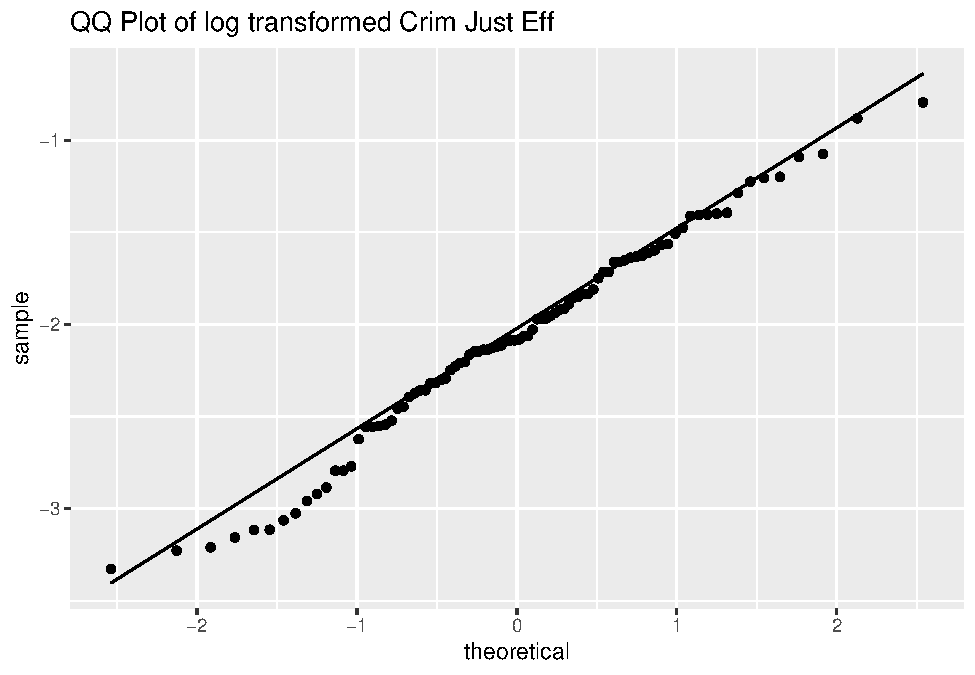
\includegraphics{Bagnard_Gaustad_Hartman_Leung_Lab_3_files/figure-latex/unnamed-chunk-57-1.pdf}

\hypertarget{model-1-linear-model}{%
\subsubsection{Model 1 Linear Model}\label{model-1-linear-model}}

We now turn to the definition of our model in terms of the variables we
operationalized, and we perform our linear regression.

\[ log(Crime Rate) = B_0 + B_1log(Scaled Wages) + B_2log(Criminal Justice Effectiveness) + B_3West + B_4Central\]

\begin{Shaded}
\begin{Highlighting}[]
\CommentTok{#dfCrime$unweighted_avg_wage <- dfCrime$scaledWages/9}
\NormalTok{model1 <-}\StringTok{ }\KeywordTok{lm}\NormalTok{(logcrmrte }\OperatorTok{~}\StringTok{ }\NormalTok{logScaledWages }\OperatorTok{+}\StringTok{ }\NormalTok{logcrimJustEff }\OperatorTok{+}\StringTok{ }\NormalTok{west }\OperatorTok{+}\StringTok{ }\NormalTok{central, }\DataTypeTok{data=}\NormalTok{dfCrime)}
\NormalTok{model1 }\CommentTok{# Coefficients}
\end{Highlighting}
\end{Shaded}

\begin{verbatim}

Call:
lm(formula = logcrmrte ~ logScaledWages + logcrimJustEff + west + 
    central, data = dfCrime)

Coefficients:
   (Intercept)  logScaledWages  logcrimJustEff            west  
      -15.8272          1.9933         -0.4792         -0.5916  
       central  
       -0.2423  
\end{verbatim}

\begin{Shaded}
\begin{Highlighting}[]
\KeywordTok{summary}\NormalTok{(model1)}\OperatorTok{$}\NormalTok{adj.r.square }\CommentTok{# Adjusted R^2 value.}
\end{Highlighting}
\end{Shaded}

\begin{verbatim}
[1] 0.6334827
\end{verbatim}

\textbf{Cook's Distance (Leverage/Influence) Analysis}\\
None of the points approach a Cook's distance of concern. Some of the
higher leveraged points do trend towards larger negative residuals. This
suggests that our model might not be capturing a phenomenon at more
extreme values of the regressors. For an initial model there is nothing
of major concern.

\begin{Shaded}
\begin{Highlighting}[]
\KeywordTok{plot}\NormalTok{(model1, }\DataTypeTok{which=}\DecValTok{5}\NormalTok{) }\CommentTok{# Variance Inflation Factor}
\end{Highlighting}
\end{Shaded}

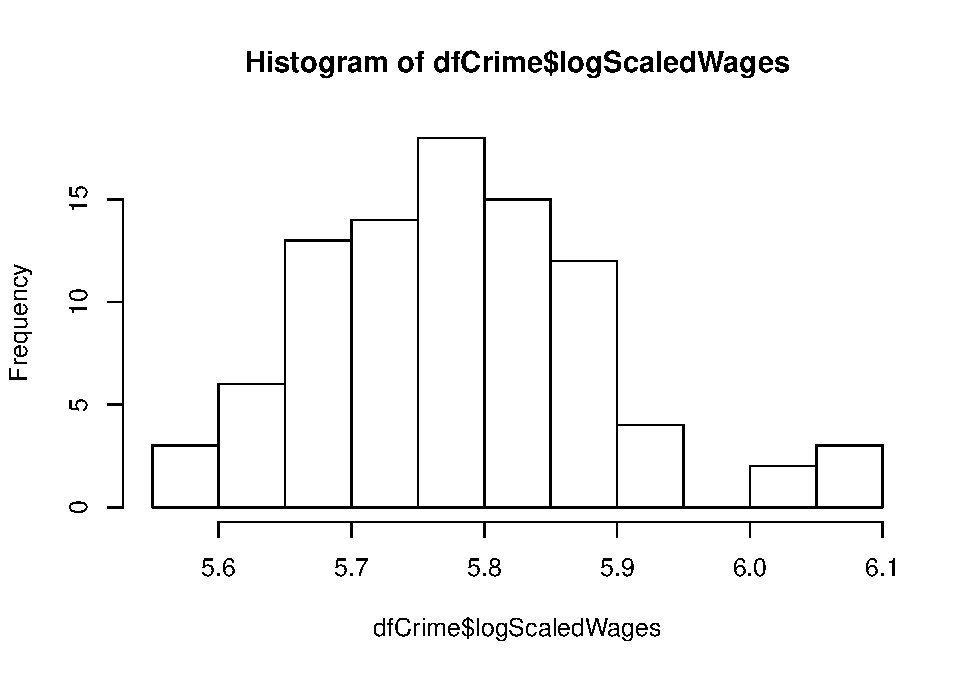
\includegraphics{Bagnard_Gaustad_Hartman_Leung_Lab_3_files/figure-latex/unnamed-chunk-59-1.pdf}

\textbf{Model 1 CLM Assumptions:}\\
* \textbf{MLR1} Linear in parameters: The model has had its data
transformed as described above to allow a linear fit of the model.

\begin{itemize}
\item
  \textbf{MLR2} Random Sampling: The data is collected from a data set
  with rolled up data for each county. We cannot comment on the
  randomness of the samples, though nearly all counties are represented
  in North Carolina.
\item
  \textbf{MLR3} No perfect multicollinearity: None of the variables
  chosen for the model are constant or perfectly collinear as the
  economy and criminal justice effectiveness are independent. Our low
  VIF value shows very little collinearity, as would be expected from
  the diverse and limited variables included in the model.
\end{itemize}

\begin{Shaded}
\begin{Highlighting}[]
\KeywordTok{vif}\NormalTok{(model1) }\CommentTok{# Variance Inflation Factor}
\end{Highlighting}
\end{Shaded}

\begin{verbatim}
logScaledWages logcrimJustEff           west        central 
      1.206141       1.048672       1.233732       1.413046 
\end{verbatim}

\begin{itemize}
\item
  \textbf{MLR4'} The expectation of u is 0. This is difficult to prove
  in a data set like this one. It is possible that there are serious
  bias issues in the way crimes are reported and wages are recorded.
  However, if one agrees that the data has integrity and that the basic
  model presented for predicting crime rate is acceptable, then
  exogeneity can be accepted.
\item
  \textbf{MLR4} The zero conditional mean assumption is well supported
  when viewing the Residuals vs fitted plot. The spline fit is nearly
  flat and centered very close to zero.
\end{itemize}

\begin{Shaded}
\begin{Highlighting}[]
\KeywordTok{plot}\NormalTok{(model1, }\DataTypeTok{which=}\DecValTok{1}\NormalTok{)}
\end{Highlighting}
\end{Shaded}

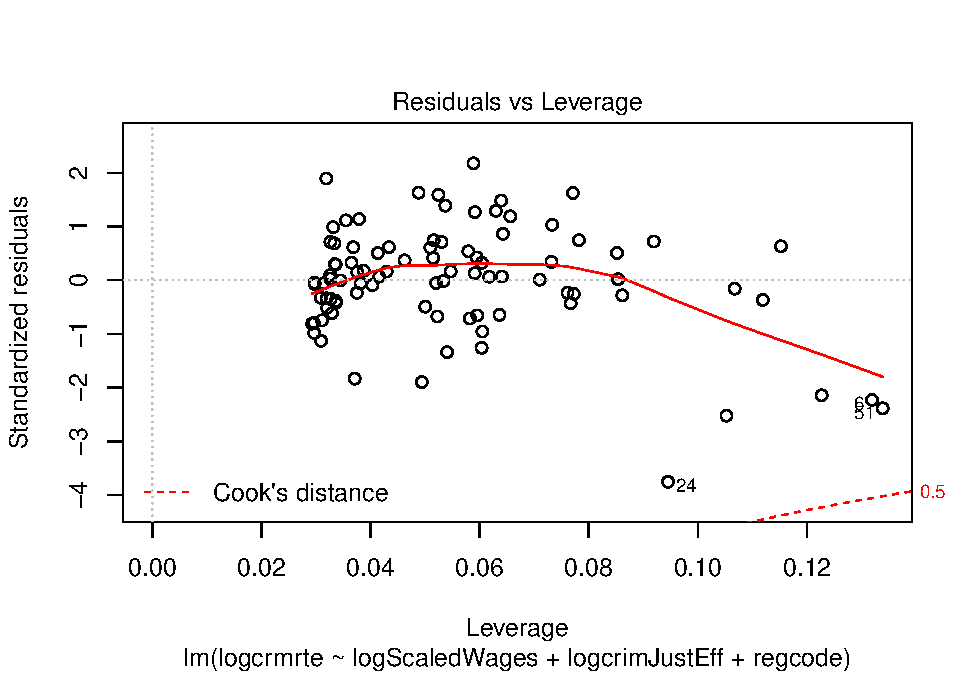
\includegraphics{Bagnard_Gaustad_Hartman_Leung_Lab_3_files/figure-latex/unnamed-chunk-61-1.pdf}

\begin{itemize}
\tightlist
\item
  \textbf{MLR5} Although there does appear to be visible heteroskedacity
  in the `lips' appearance of the Residuals vs fitted plot, a
  Breusch-Pagan test (below) confirms there is not. However, to be
  conservative and consistent we will proceed with heteroskedastic
  robust errors.
\end{itemize}

\begin{Shaded}
\begin{Highlighting}[]
\KeywordTok{bptest}\NormalTok{(model1)}
\end{Highlighting}
\end{Shaded}

\begin{verbatim}
## 
##  studentized Breusch-Pagan test
## 
## data:  model1
## BP = 4.9509, df = 4, p-value = 0.2924
\end{verbatim}

\begin{Shaded}
\begin{Highlighting}[]
\KeywordTok{coeftest}\NormalTok{(model1, }\DataTypeTok{vcov=}\NormalTok{vcovHC) }\CommentTok{#coefficients with heteroskedastic consistent standard errors}
\end{Highlighting}
\end{Shaded}

\begin{verbatim}
## 
## t test of coefficients:
## 
##                  Estimate Std. Error t value  Pr(>|t|)    
## (Intercept)    -15.827185   2.672144 -5.9230 6.520e-08 ***
## logScaledWages   1.993331   0.489061  4.0758 0.0001027 ***
## logcrimJustEff  -0.479168   0.104765 -4.5737 1.617e-05 ***
## west            -0.591604   0.102146 -5.7917 1.144e-07 ***
## central         -0.242262   0.081184 -2.9841 0.0037123 ** 
## ---
## Signif. codes:  0 '***' 0.001 '**' 0.01 '*' 0.05 '.' 0.1 ' ' 1
\end{verbatim}

\begin{itemize}
\tightlist
\item
  \textbf{MLR6} The final assumption of linear regression is that the
  errors are normally distributed. This appears to hold for the bulk of
  the residuals, however, there is skewness on the tails. This
  non-normality is also reflected in the significant return on the
  Shapiro test. But our high sample size allows us to leverage the
  Central Limit Theorem and assume normally distributed errors.
\end{itemize}

\begin{Shaded}
\begin{Highlighting}[]
\KeywordTok{shapiro.test}\NormalTok{(model1}\OperatorTok{$}\NormalTok{residuals) }\CommentTok{# test for normality}
\end{Highlighting}
\end{Shaded}

\begin{verbatim}

    Shapiro-Wilk normality test

data:  model1$residuals
W = 0.95925, p-value = 0.00652
\end{verbatim}

\begin{Shaded}
\begin{Highlighting}[]
\KeywordTok{plot}\NormalTok{(model1, }\DataTypeTok{which=}\DecValTok{2}\NormalTok{) }\CommentTok{# QQ plot for residuals}
\end{Highlighting}
\end{Shaded}

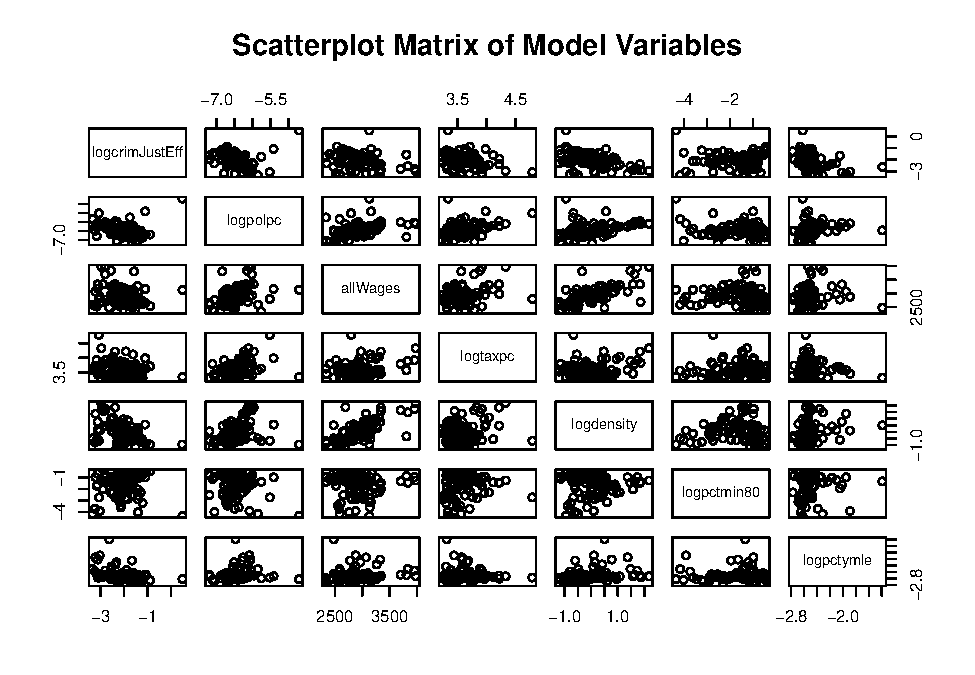
\includegraphics{Bagnard_Gaustad_Hartman_Leung_Lab_3_files/figure-latex/unnamed-chunk-63-1.pdf}

\hypertarget{model-1-interpretation}{%
\subsubsection{Model 1 Interpretation}\label{model-1-interpretation}}

The model 1 gives estimates and standard errors that are heteroskedastic
consistent. All the coefficients are found to be statistically
significant. The coefficient of the log of scaled average wage is
calculated to be \textasciitilde{}2. This means that an increase of 1\%
in wages is correlated with an increase of 2\% in crime rate. Generally
speaking, increased wages are not normally associated with increased
crime. This suggests that wages are correlated with stronger omitted
variables that affects crime. Another aspect that may be missed in our
operationlized variable is the economic inequality in the county.
Averages are easily affected by extreme values. It is possible there are
very high earners that can influence a sector's average wage, but don't
represent the bulk of workers. Further, there is no understanding of the
weighting for each sector. For example, one sector, like telecom, may
have high wages in a county but not have very many workers, further
demonstrating inequality. This detail is missed when each sector is
rolled into a single average and then scaled with all other sector
averages. However, the significant result of wage on crime suggests that
we are capturing some cause of crime that is correlated to wages. We
will continue to monitor how wage changes as a predictor when we
introduce more regressors.

Criminal justice effectiveness (convictions/crime) is has a coefficient
of around 0.5 which suggests that an increase of 1\% increase in
convictions per crime will decrease crime by nearly .5\%. This suggests
that we have found a relatively strong correlation and constructed a
good operationalization of a county's criminal justice effect on crime
rate. This variable will be monitored as we add more regressors.

Region dummy variables of West and Central are both significant. This
suggests that regionally, there are differences that are not captured by
the Wages and Criminal Justice Effectiveness variable that affect crime.
While the West and Central regions both have lower crime than the
Coastal/Other region, the West is much more pronounced with a value of
around 0.6. This suggests that when correcting for differences in
Criminal Justice Effectiveness and Wages, the west will still have crime
rate lower by about 60\%.

Overall, the model shows a moderately good fit, with an adjusted R
square of 0.63. This can be interpreted as: the model explains 63\% of
the variation in crime. In the next model we will try to improve our
operationalization of economics and criminal justice by investigating
police per capita and tax revenue per capita.

\hypertarget{model-2}{%
\subsection{Model 2}\label{model-2}}

\hypertarget{introduction-2}{%
\subsubsection{Introduction}\label{introduction-2}}

In this model, we introduce the additional covariates of tax per capita
(taxpc) and police per capita (polpc) to give us more insight into our
economic and law enforcement related variables.

\begin{itemize}
\item
  \textbf{Police Per Capita}\\
  The Police Per Capita in a county can be influential on the Criminal
  Justice Effectiveness. With more police in a given area, one would
  assume that crime rates would decrease, however, as we mentioned
  earlier in our EDA, polpc has a positive correlation with crmrte.
  Including this variable in our analysis will give us more insight into
  the relationship of variables used in model 1.
\item
  \textbf{Tax Per Capita}\\
  The Tax Per Capita can have a direct impact on the Police Per Capita.
  A higher tax per capita means that the county has more revenue to
  spend on public services like the police force (ie. increasing the
  number of police in the county). This positive correlation
  relationship can be seen in our prior introductory data analysis.
  However, taxpc may also serve as an inidication of economic health as
  well. The largest sources of tax revenues are the individual income
  tax and payroll taxes, followed by the corporate income tax. As a
  result, by including taxpc in our model will give us additional
  insight into our economic variables.
\end{itemize}

\hypertarget{model-2-eda-and-data-transformations}{%
\subsubsection{Model 2 EDA and Data
Transformations}\label{model-2-eda-and-data-transformations}}

Before we create our model, we will analyze each of the additional
variables to see if transformations are needed.

To start, we will look at the polpc variable:

\begin{Shaded}
\begin{Highlighting}[]
\NormalTok{p1 <-}\StringTok{ }\KeywordTok{ggplot}\NormalTok{(dfCrime, }\KeywordTok{aes}\NormalTok{(}\DataTypeTok{x =}\NormalTok{ polpc, }\DataTypeTok{color=}\NormalTok{regcode, }\DataTypeTok{fill =}\NormalTok{ regcode)) }\OperatorTok{+}
\StringTok{  }\KeywordTok{geom_histogram}\NormalTok{(}\DataTypeTok{position=}\StringTok{"identity"}\NormalTok{, }\DataTypeTok{alpha=}\FloatTok{0.5}\NormalTok{, }\DataTypeTok{bins=}\DecValTok{30}\NormalTok{) }\OperatorTok{+}
\StringTok{  }\KeywordTok{labs}\NormalTok{(}\DataTypeTok{title=}\StringTok{"Police per Capita"}\NormalTok{, }\DataTypeTok{x=}\StringTok{"Police per Capita"}\NormalTok{, }\DataTypeTok{y=}\StringTok{"Count"}\NormalTok{)}
\NormalTok{p2 <-}\StringTok{ }\KeywordTok{ggplot}\NormalTok{(dfCrime, }\KeywordTok{aes}\NormalTok{(}\DataTypeTok{x =} \KeywordTok{log}\NormalTok{(polpc), }\DataTypeTok{color=}\NormalTok{regcode, }\DataTypeTok{fill =}\NormalTok{ regcode)) }\OperatorTok{+}
\StringTok{  }\KeywordTok{geom_histogram}\NormalTok{(}\DataTypeTok{position=}\StringTok{"identity"}\NormalTok{, }\DataTypeTok{alpha=}\FloatTok{0.5}\NormalTok{, }\DataTypeTok{bins=}\DecValTok{30}\NormalTok{) }\OperatorTok{+}
\StringTok{  }\KeywordTok{labs}\NormalTok{(}\DataTypeTok{title=}\StringTok{"Log Transformed Police per Capita"}\NormalTok{, }\DataTypeTok{x=}\StringTok{"Log(Police per Capita)"}\NormalTok{, }\DataTypeTok{y=}\StringTok{"Count"}\NormalTok{)}
\KeywordTok{grid.arrange}\NormalTok{(p1, p2, }\DataTypeTok{ncol=}\DecValTok{2}\NormalTok{)}
\end{Highlighting}
\end{Shaded}

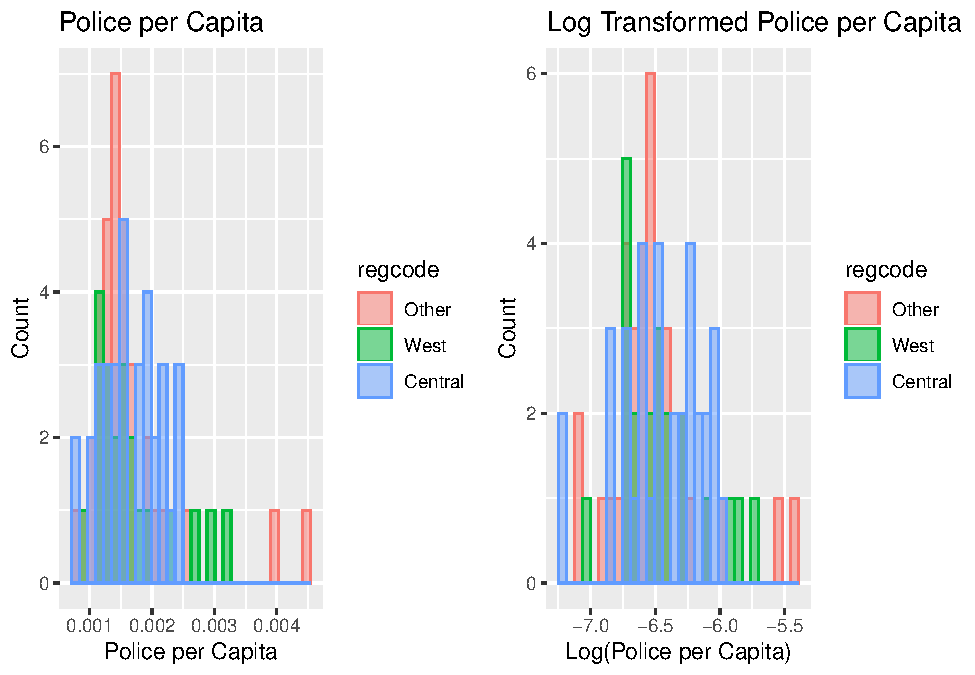
\includegraphics{Bagnard_Gaustad_Hartman_Leung_Lab_3_files/figure-latex/unnamed-chunk-64-1.pdf}

As we can see from the histograms above, taking the natural log of polpc
brings its distribution closer to normal. As a result, we will use the
log(polpc) in our analysis.

\begin{Shaded}
\begin{Highlighting}[]
\CommentTok{# creating the logpolpc variable}
\NormalTok{dfCrime}\OperatorTok{$}\NormalTok{logpolpc <-}\StringTok{ }\KeywordTok{log}\NormalTok{(dfCrime}\OperatorTok{$}\NormalTok{polpc)}
\end{Highlighting}
\end{Shaded}

Next, we will take a look at our taxpc variable to see if a
transformation is warranted:

\begin{Shaded}
\begin{Highlighting}[]
\NormalTok{p1 <-}\StringTok{ }\KeywordTok{ggplot}\NormalTok{(dfCrime, }\KeywordTok{aes}\NormalTok{(}\DataTypeTok{x =}\NormalTok{ taxpc, }\DataTypeTok{color=}\NormalTok{regcode, }\DataTypeTok{fill =}\NormalTok{ regcode)) }\OperatorTok{+}
\StringTok{  }\KeywordTok{geom_histogram}\NormalTok{(}\DataTypeTok{position=}\StringTok{"identity"}\NormalTok{, }\DataTypeTok{alpha=}\FloatTok{0.5}\NormalTok{, }\DataTypeTok{bins=}\DecValTok{30}\NormalTok{) }\OperatorTok{+}
\StringTok{  }\KeywordTok{labs}\NormalTok{(}\DataTypeTok{title=}\StringTok{"Tax revenue per capita"}\NormalTok{, }\DataTypeTok{x=}\StringTok{"Tax revenue per Capita"}\NormalTok{, }\DataTypeTok{y=}\StringTok{"Count"}\NormalTok{)}
\NormalTok{p2 <-}\StringTok{ }\KeywordTok{ggplot}\NormalTok{(dfCrime, }\KeywordTok{aes}\NormalTok{(}\DataTypeTok{x =} \KeywordTok{log}\NormalTok{(taxpc), }\DataTypeTok{color=}\NormalTok{regcode, }\DataTypeTok{fill =}\NormalTok{ regcode)) }\OperatorTok{+}
\StringTok{  }\KeywordTok{geom_histogram}\NormalTok{(}\DataTypeTok{position=}\StringTok{"identity"}\NormalTok{, }\DataTypeTok{alpha=}\FloatTok{0.5}\NormalTok{, }\DataTypeTok{bins=}\DecValTok{30}\NormalTok{) }\OperatorTok{+}
\StringTok{  }\KeywordTok{labs}\NormalTok{(}\DataTypeTok{title=}\StringTok{"Log Transformed Tax revenue per Capita"}\NormalTok{, }\DataTypeTok{x=}\StringTok{"Log(Tax revenue per Capita)"}\NormalTok{, }\DataTypeTok{y=}\StringTok{"Count"}\NormalTok{)}
\KeywordTok{grid.arrange}\NormalTok{(p1, p2, }\DataTypeTok{ncol=}\DecValTok{2}\NormalTok{)}
\end{Highlighting}
\end{Shaded}

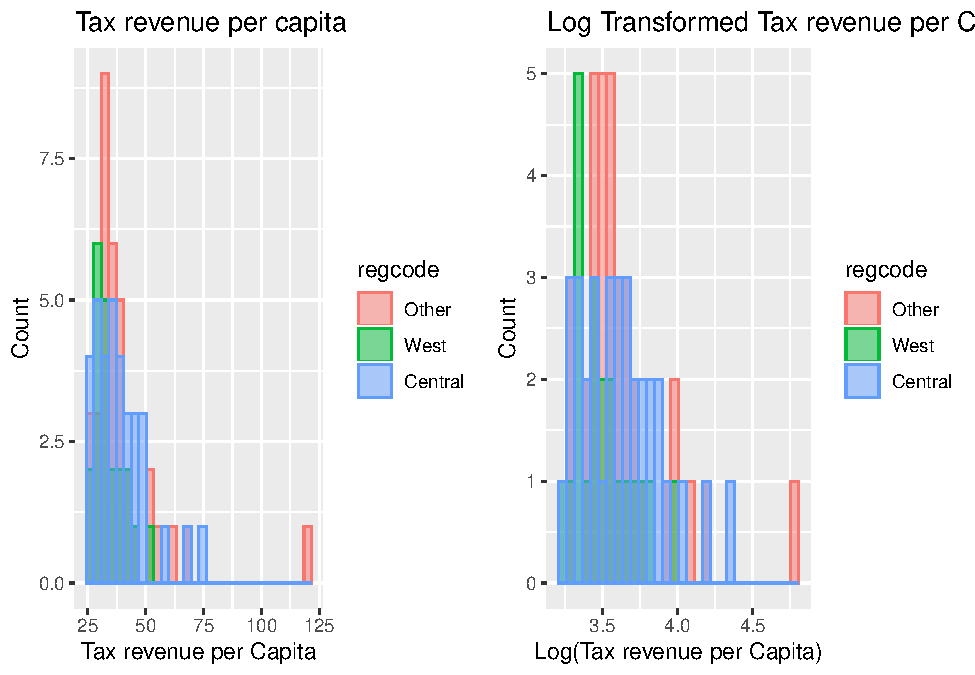
\includegraphics{Bagnard_Gaustad_Hartman_Leung_Lab_3_files/figure-latex/unnamed-chunk-66-1.pdf}
The histogram of taxpc, depicts each region as having an approximately
normal distribution with each centered on a different mean. When we take
the natural log of taxpc, we can see in the histogram, above, that each
region has a more normal distribution. In addition, taking the natural
log of taxpc reduces the extremity of the outlier seen in histogram of
taxpc. We will use the log(taxpc) in our analysis.

\begin{Shaded}
\begin{Highlighting}[]
\NormalTok{dfCrime}\OperatorTok{$}\NormalTok{logtaxpc <-}\StringTok{ }\KeywordTok{log}\NormalTok{(dfCrime}\OperatorTok{$}\NormalTok{taxpc)}
\end{Highlighting}
\end{Shaded}

Now that we have transformed our variables, we will take a look at how
they relate to crime rate, and if the trends vary between each region.

\begin{Shaded}
\begin{Highlighting}[]
\NormalTok{logpolpc_plot<-}\KeywordTok{ggplot}\NormalTok{(}\DataTypeTok{data =}\NormalTok{ dfCrime, }\KeywordTok{aes}\NormalTok{(}\DataTypeTok{x =}\NormalTok{ logpolpc, }\DataTypeTok{y =}\NormalTok{ logcrmrte, }\DataTypeTok{color =}\NormalTok{ regcode)) }\OperatorTok{+}
\StringTok{      }\KeywordTok{geom_point}\NormalTok{()}\OperatorTok{+}
\StringTok{  }\KeywordTok{geom_smooth}\NormalTok{(}\DataTypeTok{method =} \StringTok{"lm"}\NormalTok{)}
\NormalTok{logtaxpc_plot<-}\KeywordTok{ggplot}\NormalTok{(}\DataTypeTok{data =}\NormalTok{ dfCrime, }\KeywordTok{aes}\NormalTok{(}\DataTypeTok{x =}\NormalTok{ logtaxpc, }\DataTypeTok{y =}\NormalTok{ logcrmrte, }\DataTypeTok{color =}\NormalTok{ regcode)) }\OperatorTok{+}
\StringTok{      }\KeywordTok{geom_point}\NormalTok{()}\OperatorTok{+}
\StringTok{  }\KeywordTok{geom_smooth}\NormalTok{(}\DataTypeTok{method =} \StringTok{"lm"}\NormalTok{)}

\KeywordTok{options}\NormalTok{(}\DataTypeTok{repr.plot.width=}\DecValTok{8}\NormalTok{, }\DataTypeTok{repr.plot.height=}\DecValTok{16}\NormalTok{)}
\KeywordTok{grid.arrange}\NormalTok{(logpolpc_plot,logtaxpc_plot, }\DataTypeTok{ncol=}\DecValTok{2}\NormalTok{)}
\end{Highlighting}
\end{Shaded}

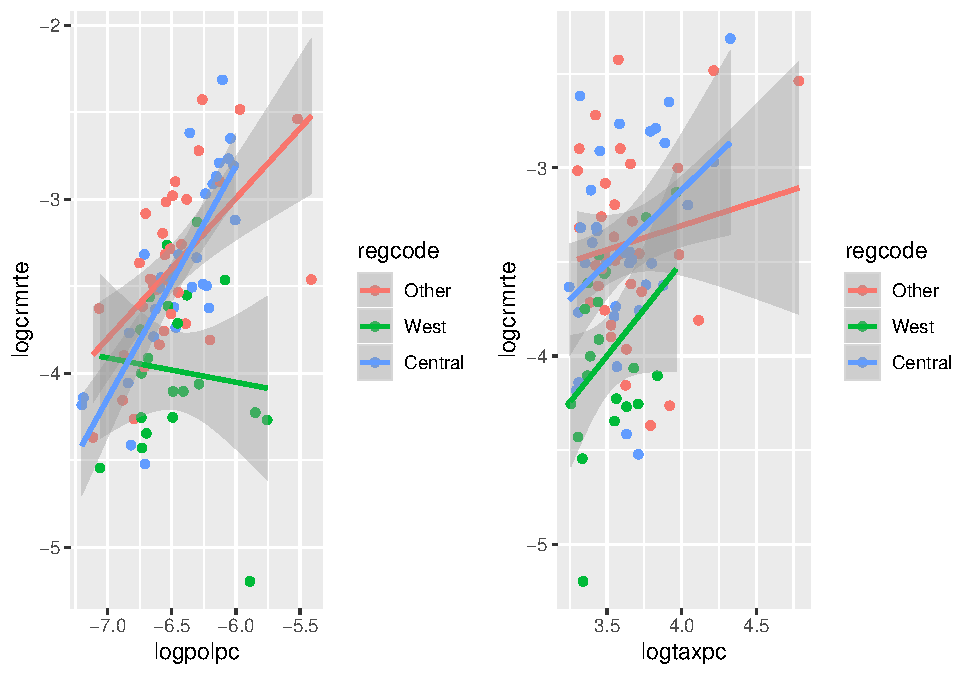
\includegraphics{Bagnard_Gaustad_Hartman_Leung_Lab_3_files/figure-latex/unnamed-chunk-68-1.pdf}

Right away, we can see clear difference between each region. The
``Other'' and ``Central'' regions have positively sloped regression
lines against police per capita, while ``West'' has a negatively sloped
regression line. This suggests that we should investigate interactions
between police per capita and the regions in our model.

The tax per capita relationship, on the other hand, does not demonstrate
the same slope variation between each regions. As result, we will not
look into the interactions between tax per capita and regions in our
model.

\hypertarget{model-2-linear-model}{%
\subsubsection{Model 2 Linear Model}\label{model-2-linear-model}}

\[logcrmrte = \beta_0 + \beta_1log(Scaled Wages) + \beta_2log(Criminal Justice Effectiveness) + \beta_3West + \beta_4Central + \beta_5log(Police Per Capita)*West\\ +  \beta_6log(Police Per Capita)*Central  + \beta_7log((Police Per Capita) + \beta_8log(Tax Per Capita) + u\]

\begin{Shaded}
\begin{Highlighting}[]
\NormalTok{model2 <-}\StringTok{ }\KeywordTok{lm}\NormalTok{(logcrmrte }\OperatorTok{~}\StringTok{ }\NormalTok{logScaledWages }\OperatorTok{+}\StringTok{ }\NormalTok{logcrimJustEff }\OperatorTok{+}\StringTok{ }\NormalTok{logpolpc}\OperatorTok{*}\NormalTok{west }\OperatorTok{+}\StringTok{ }\NormalTok{logpolpc}\OperatorTok{*}\NormalTok{central }\OperatorTok{+}\StringTok{ }\NormalTok{logtaxpc, }\DataTypeTok{data =}\NormalTok{ dfCrime)}
\NormalTok{model2}
\end{Highlighting}
\end{Shaded}

\begin{verbatim}

Call:
lm(formula = logcrmrte ~ logScaledWages + logcrimJustEff + logpolpc * 
    west + logpolpc * central + logtaxpc, data = dfCrime)

Coefficients:
     (Intercept)    logScaledWages    logcrimJustEff          logpolpc  
         -6.9023            1.1912           -0.4230            0.5624  
            west           central          logtaxpc     logpolpc:west  
         -5.9526            1.0020           -0.1504           -0.8249  
logpolpc:central  
          0.1857  
\end{verbatim}

\begin{Shaded}
\begin{Highlighting}[]
\KeywordTok{summary}\NormalTok{(model2)}\OperatorTok{$}\NormalTok{adj.r.square}
\end{Highlighting}
\end{Shaded}

\begin{verbatim}
[1] 0.7003473
\end{verbatim}

From the Residuals vs Leverage graph, below, we can see that our model
does not contain any outliers with have significant influence (ie. there
are no points with a Cook's distance of 0.5 or greater).

\begin{Shaded}
\begin{Highlighting}[]
\KeywordTok{plot}\NormalTok{(model2, }\DataTypeTok{which=}\DecValTok{5}\NormalTok{)}
\end{Highlighting}
\end{Shaded}

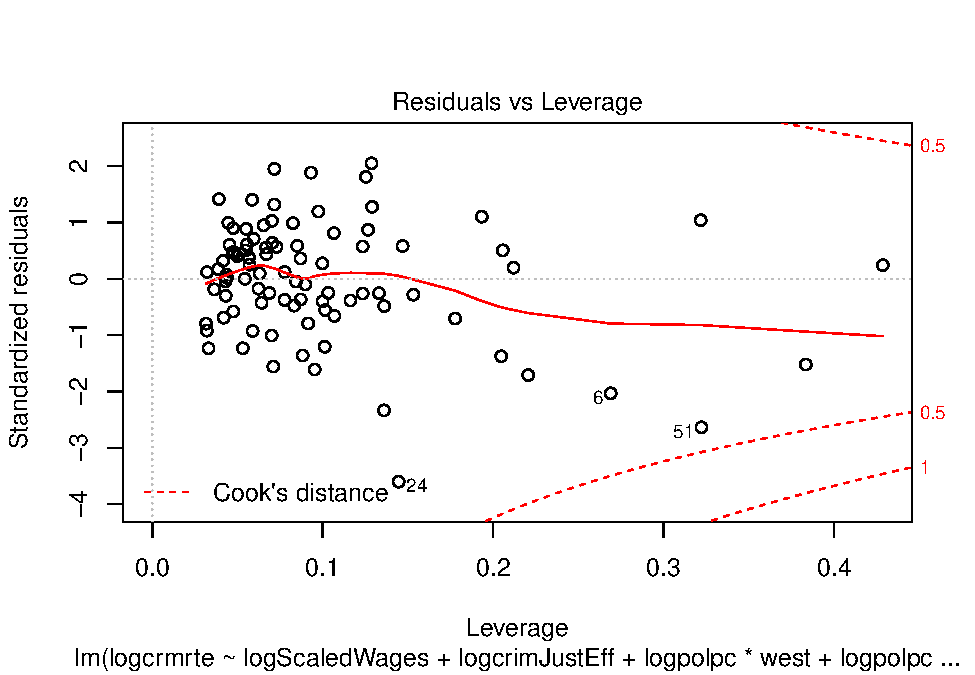
\includegraphics{Bagnard_Gaustad_Hartman_Leung_Lab_3_files/figure-latex/unnamed-chunk-70-1.pdf}

\textbf{Model 2 CLM Assumptions:}

\begin{itemize}
\item
  \textbf{MLR1} Discussed above.
\item
  \textbf{MLR2} Discussed above.
\item
  \textbf{MLR3: Non-perfect Collinearity} We will use the VIF function
  to provide evidence that our variables in model2 are not perfectly
  multicollinear. As we can see from the VIF results, below, all of the
  variables' values are less than five, which allows us to conclude
  model2 is free from multicollinearity.
\end{itemize}

\begin{Shaded}
\begin{Highlighting}[]
\KeywordTok{vif}\NormalTok{(model2)}
\end{Highlighting}
\end{Shaded}

\begin{verbatim}
##   logScaledWages   logcrimJustEff         logpolpc             west 
##         1.580269         1.204167         3.205590       524.364550 
##          central         logtaxpc    logpolpc:west logpolpc:central 
##       511.833903         1.433158       521.004355       507.469272
\end{verbatim}

\begin{itemize}
\tightlist
\item
  \textbf{MLR4: Zero Conditional Mean} The residual vs.~fitted chart,
  below, gives us evidence that we meet the zero conditional mean
  assumption as the majority of the residual means lie close to zero.
  The exceptions to this trend, lie on the left and right sides of the
  chart where there are fewer data points (evidence for
  heteroskedasticity - see MLR5, below).
\end{itemize}

\begin{Shaded}
\begin{Highlighting}[]
\KeywordTok{plot}\NormalTok{(model2, }\DataTypeTok{which=}\DecValTok{1}\NormalTok{)}
\end{Highlighting}
\end{Shaded}

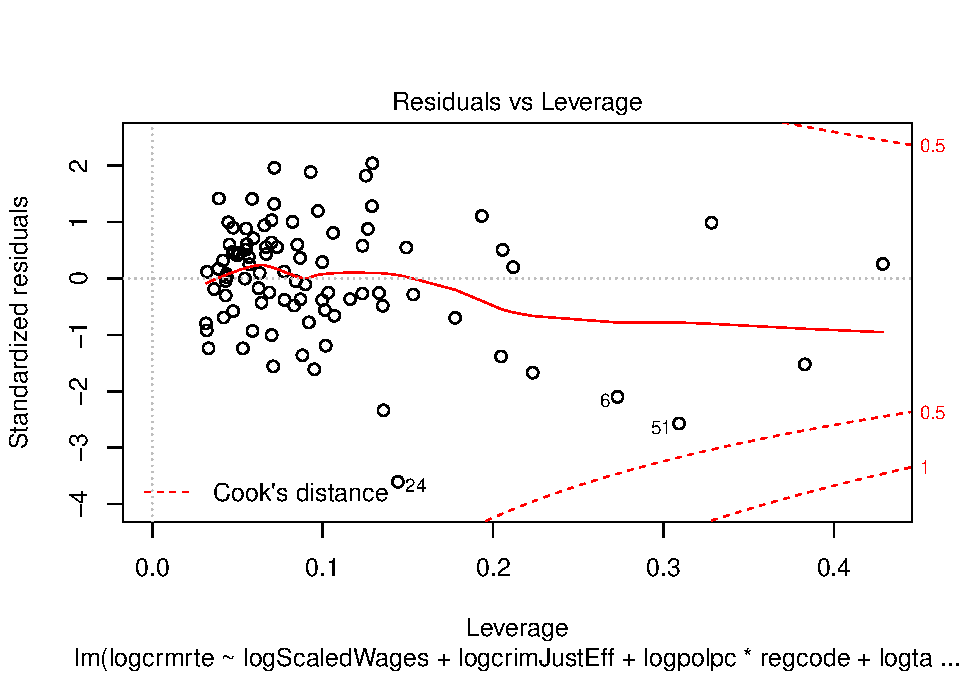
\includegraphics{Bagnard_Gaustad_Hartman_Leung_Lab_3_files/figure-latex/unnamed-chunk-72-1.pdf}

\begin{itemize}
\tightlist
\item
  \textbf{MLR5: heteroskedasticity} The above Residuals vs Fitted graph
  provides evidence of heteroskedasticity as right and left sides of the
  chart have fewer date points, and further suggested by the
  Breusch-Pagan test. Since we have evidence of heteroskedasticity, we
  will use the White-Huber method with vcovHC to generate coefficients
  that are robust to heteroskedasticity
\end{itemize}

\begin{Shaded}
\begin{Highlighting}[]
\KeywordTok{bptest}\NormalTok{(model2)}
\end{Highlighting}
\end{Shaded}

\begin{verbatim}

    studentized Breusch-Pagan test

data:  model2
BP = 14.841, df = 8, p-value = 0.06231
\end{verbatim}

\begin{Shaded}
\begin{Highlighting}[]
\KeywordTok{coeftest}\NormalTok{(model2, }\DataTypeTok{vcov=}\NormalTok{vcovHC)}
\end{Highlighting}
\end{Shaded}

\begin{verbatim}

t test of coefficients:

                 Estimate Std. Error t value  Pr(>|t|)    
(Intercept)      -6.90227    3.60175 -1.9164 0.0588457 .  
logScaledWages    1.19123    0.47430  2.5116 0.0140072 *  
logcrimJustEff   -0.42305    0.10673 -3.9638 0.0001581 ***
logpolpc          0.56237    0.25317  2.2213 0.0291213 *  
west             -5.95256    2.97585 -2.0003 0.0488196 *  
central           1.00204    1.43482  0.6984 0.4869471    
logtaxpc         -0.15038    0.19024 -0.7904 0.4315835    
logpolpc:west    -0.82487    0.45513 -1.8124 0.0736323 .  
logpolpc:central  0.18569    0.21966  0.8453 0.4004127    
---
Signif. codes:  0 '***' 0.001 '**' 0.01 '*' 0.05 '.' 0.1 ' ' 1
\end{verbatim}

As we can see from the coeftest results above, the interaction between
logpolpc and west are slightly significant while the interaction between
logpolpc and central is not statistically significant.

However, they may be jointly significant. We will run a F-test to see if
this might be the case:

\begin{Shaded}
\begin{Highlighting}[]
\KeywordTok{linearHypothesis}\NormalTok{(model2, }\KeywordTok{c}\NormalTok{(}\StringTok{"logpolpc:west=0"}\NormalTok{, }\StringTok{"logpolpc:central=0"}\NormalTok{), }\DataTypeTok{vcov=}\NormalTok{vcovHC)}
\end{Highlighting}
\end{Shaded}

\begin{verbatim}
## Linear hypothesis test
## 
## Hypothesis:
## logpolpc:west = 0
## logpolpc:central = 0
## 
## Model 1: restricted model
## Model 2: logcrmrte ~ logScaledWages + logcrimJustEff + logpolpc * west + 
##     logpolpc * central + logtaxpc
## 
## Note: Coefficient covariance matrix supplied.
## 
##   Res.Df Df      F  Pr(>F)  
## 1     83                    
## 2     81  2 3.0723 0.05175 .
## ---
## Signif. codes:  0 '***' 0.001 '**' 0.01 '*' 0.05 '.' 0.1 ' ' 1
\end{verbatim}

We can see frome the F-test, above, that the interactions between
logpolpc and the dummy variables west and central are not quite
statistically significant to our model. However, we will continue to
look at the standalone effects of west and central and keep them for our
third model.

\begin{Shaded}
\begin{Highlighting}[]
\KeywordTok{linearHypothesis}\NormalTok{(model2, }\KeywordTok{c}\NormalTok{(}\StringTok{"logpolpc=0"}\NormalTok{, }\StringTok{"logtaxpc=0"}\NormalTok{), }\DataTypeTok{vcov=}\NormalTok{vcovHC)}
\end{Highlighting}
\end{Shaded}

\begin{verbatim}
## Linear hypothesis test
## 
## Hypothesis:
## logpolpc = 0
## logtaxpc = 0
## 
## Model 1: restricted model
## Model 2: logcrmrte ~ logScaledWages + logcrimJustEff + logpolpc * west + 
##     logpolpc * central + logtaxpc
## 
## Note: Coefficient covariance matrix supplied.
## 
##   Res.Df Df      F  Pr(>F)  
## 1     83                    
## 2     81  2 2.6478 0.07693 .
## ---
## Signif. codes:  0 '***' 0.001 '**' 0.01 '*' 0.05 '.' 0.1 ' ' 1
\end{verbatim}

We also see that logtaxpc and logpolpc together are not jointly
significant. Seeing how logtaxpc is also not individually significant we
will dismiss it from inclusion in our third model. However, we will
continue to investigate the standalone effects of west and central and
keep them for our third model.

\begin{itemize}
\tightlist
\item
  \textbf{MLR6: Normal Distribution of Errors} The Normal Q-Q plot,
  below, provides evidence that our residuals follow a normal
  distribution. While there are some data points on the left and right
  side of the graph that stray from the diagonal line, since our data
  set has over 30 datapoints, per the CLT, we can assume residuals have
  a normal distribution.
\end{itemize}

\begin{Shaded}
\begin{Highlighting}[]
\KeywordTok{plot}\NormalTok{(model2, }\DataTypeTok{which=}\DecValTok{2}\NormalTok{)}
\end{Highlighting}
\end{Shaded}

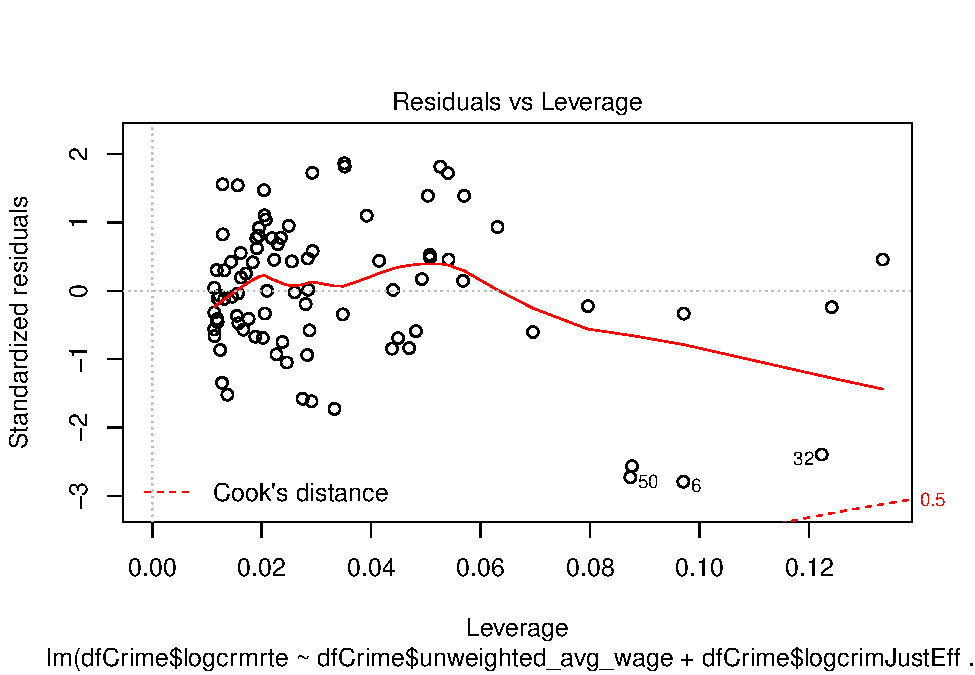
\includegraphics{Bagnard_Gaustad_Hartman_Leung_Lab_3_files/figure-latex/unnamed-chunk-76-1.pdf}

\hypertarget{model-2-interpretation}{%
\subsubsection{Model 2 Interpretation}\label{model-2-interpretation}}

The Adjusted R-squared variable penalizes for additional variables,
which means there is a chance that this value will decrease if the added
variables do not contribute to the model. By comparing the Adjusted
R-squared value between our first and second models, we see that
logtaxpc and the interaction between logpolpc and regcode help describe
logcrmrte.

Our second model has an Adjusted R-squared value of approx 0.70, which
means 70\% of the variation in the natural log of the crime rate is
explained by the explanatory variables used in this model. This is a
slight increase compared to our first model, that has an Adjusted
R-squared value that explaines 63\% of the model.

Coefficient Analysis (assuming ceterus paribus): - logcrimJustEff: If we
were to increase criminal justice efficiency by 1\%, we would expect the
crime rate to decrease by approximately 0.42\%. - logpolpc: If we were
to increase police per capita by 1\%, we would expect the crime rate to
increase by approximately 0.56\%. - logScaledWages: If we were to
increase average wages by 1\%, we would expect the crime rate to
increase by approximately 1.2\%. - taxpc: If we were to increase tax per
capita by 1\%, we would expect the crime rate to decrease by
approximately 0.15\%.

Compared to model 1, the adjusted R-squared of model 2 shows improvement
from the variables selected, although interaction behavior for the
regions was less pronounced. This suggests we should continue our
analysis by focusing on the joint significance of the variables we added
in model 2, but without the regional interactions.

\hypertarget{model-3}{%
\subsection{Model 3}\label{model-3}}

\hypertarget{discussion-of-variables}{%
\subsubsection{Discussion of Variables}\label{discussion-of-variables}}

From Model 2, we noted that the addition of the transformed variable
logpolpc had statistical significance and helped improve the fit of the
model, as measured by adjusted R-squared, to 70\%. To increase our
understanding at the linkages between police presence, economic
conditions, criminal justice effectiveness and region, we propose to
also analyse the areas of demographics which could have an effect on
both of our key explanatory variables.

\textbf{Minorities}\\
One key component of demographics is the race of the county inhabitants
and how they are perceived and treated by others, especially for
minorities in the population. For example, systemic racism could have an
important effect on:\\
* Criminal Justice Effectiveness: If police, lawyers and judges are
racially biased, this could lead to more arrests and more convictions
regardless of the strength of the legal case and the evidence. As a
result, we hypothesize the crime rate would increase.\\
* Economic Opportunity: Racism could prohibit members of the minority
from having access to education, jobs and higher wages. Racism could
also limit access to healthcare and social programmes which has a
negative effect on economic opportunity.

However, since we cannot directly measure racism, we have to
operationalize this covariate by examining its effect in the real world.
We propose to use the variable pctmin80, which represents the percentage
of minorities in the population of the county. This is also a continous
parameter and so given a higher the percentage of minorities, we should
expect to see a greater effect.

From the summary and boxplot below, we can see that the percentage of
minorities ranges from 0.0154 - 0.6435, with a mean of 0.2621. We note
that there are no major outliers. In addition, different regions and
counties can have different demographics. We can see from the boxplots
below that counties in the West have a significantly lower percentage of
minorities than the other two regions.

We will apply the natural log to the variable pctmin80 to 1) make it
easier for us to interpret the coefficient in our linear model and 2) to
better expose the linear relationship in the model.

\begin{Shaded}
\begin{Highlighting}[]
\KeywordTok{summary}\NormalTok{(dfCrime}\OperatorTok{$}\NormalTok{pctmin80)}
\end{Highlighting}
\end{Shaded}

\begin{verbatim}
   Min. 1st Qu.  Median    Mean 3rd Qu.    Max. 
0.01284 0.10024 0.24852 0.25713 0.38183 0.64348 
\end{verbatim}

\begin{Shaded}
\begin{Highlighting}[]
\KeywordTok{options}\NormalTok{(}\DataTypeTok{repr.plot.width=}\DecValTok{8}\NormalTok{, }\DataTypeTok{repr.plot.height=}\DecValTok{4}\NormalTok{)}
\NormalTok{p<-}\KeywordTok{ggplot}\NormalTok{(}\DataTypeTok{data =}\NormalTok{ dfCrime, }\KeywordTok{aes}\NormalTok{(}\DataTypeTok{y =}\NormalTok{ pctmin80, }\DataTypeTok{color =}\NormalTok{ regcode)) }\OperatorTok{+}
\StringTok{     }\KeywordTok{geom_boxplot}\NormalTok{(}\DataTypeTok{show.legend=}\OtherTok{FALSE}\NormalTok{) }\OperatorTok{+}\StringTok{ }\KeywordTok{facet_wrap}\NormalTok{(}\OperatorTok{~}\StringTok{ }\NormalTok{regcode)}
\NormalTok{p2<-}\KeywordTok{ggplot}\NormalTok{(}\DataTypeTok{data =}\NormalTok{ dfCrime, }\KeywordTok{aes}\NormalTok{(}\DataTypeTok{y =}\NormalTok{ pctmin80)) }\OperatorTok{+}
\StringTok{     }\KeywordTok{geom_boxplot}\NormalTok{()}
\KeywordTok{grid.arrange}\NormalTok{(p, p2, }\DataTypeTok{ncol=}\DecValTok{2}\NormalTok{)}
\end{Highlighting}
\end{Shaded}

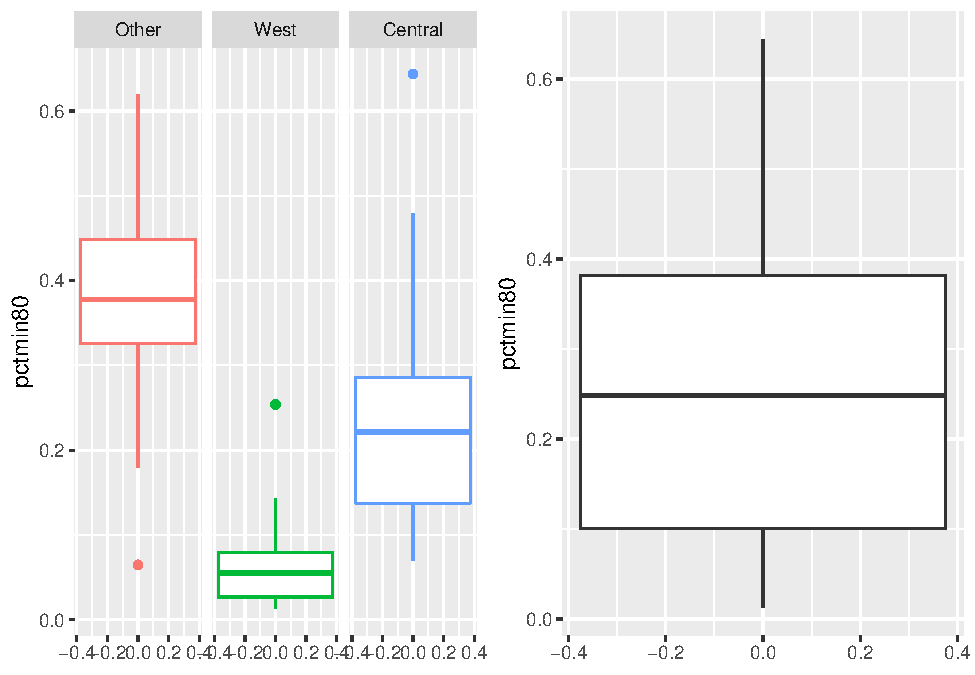
\includegraphics{Bagnard_Gaustad_Hartman_Leung_Lab_3_files/figure-latex/unnamed-chunk-77-1.pdf}

\begin{Shaded}
\begin{Highlighting}[]
\NormalTok{dfCrime}\OperatorTok{$}\NormalTok{logpctmin80 <-}\StringTok{ }\KeywordTok{log}\NormalTok{(dfCrime}\OperatorTok{$}\NormalTok{pctmin80)}
\end{Highlighting}
\end{Shaded}

\textbf{Density}\\
Another component of demographics is the population density, which can
have impacts that may be positive or negative on the crime rate:\\
* \textbf{Criminal Justice Effectiveness}: With more people in a given
area, there may be more opportunities for more people to commit crimes.
However, a higher density may also result in higher deterents such as
more eyewitnesses or faster law-enforcement response rates.\\
* \textbf{Economic Opportunity}: In high density areas, there is an
increase in demand for support services such as food, retail, utilities,
etc. As a result, there is a high demand for service jobs, which
increases the economic opportunities within the area. However, more
people in a given area, there is a closer proximity to drugs, alcohol
and gang violence - all of which are inhibitors to better economic
outcomes.

From the summary and boxplot below, we can see that the density ranges
from 0.3006 - 8.8277, with a mean of 0.9792 per square mile. We note
that while there are some outliers to the data, this does not appear at
first glance to be an issue as some counties can contain major cities
which would naturally lead to a higher population density. As a result,
we will not make adjustments to any outliers unless we detect datapoints
having high influence in our model.

\begin{Shaded}
\begin{Highlighting}[]
\KeywordTok{summary}\NormalTok{(dfCrime}\OperatorTok{$}\NormalTok{density)}
\end{Highlighting}
\end{Shaded}

\begin{verbatim}
##    Min. 1st Qu.  Median    Mean 3rd Qu.    Max. 
##  0.3006  0.5519  1.0008  1.4545  1.5880  8.8277
\end{verbatim}

\begin{Shaded}
\begin{Highlighting}[]
\KeywordTok{options}\NormalTok{(}\DataTypeTok{repr.plot.width=}\DecValTok{8}\NormalTok{, }\DataTypeTok{repr.plot.height=}\DecValTok{4}\NormalTok{)}
\NormalTok{p<-}\KeywordTok{ggplot}\NormalTok{(}\DataTypeTok{data =}\NormalTok{ dfCrime, }\KeywordTok{aes}\NormalTok{(}\DataTypeTok{y =}\NormalTok{ density, }\DataTypeTok{color =}\NormalTok{ regcode)) }\OperatorTok{+}
\StringTok{     }\KeywordTok{geom_boxplot}\NormalTok{(}\DataTypeTok{show.legend=}\OtherTok{FALSE}\NormalTok{) }\OperatorTok{+}\StringTok{ }\KeywordTok{facet_wrap}\NormalTok{(}\OperatorTok{~}\StringTok{ }\NormalTok{regcode)}
\NormalTok{p2<-}\KeywordTok{ggplot}\NormalTok{(}\DataTypeTok{data =}\NormalTok{ dfCrime, }\KeywordTok{aes}\NormalTok{(}\DataTypeTok{y =}\NormalTok{ density)) }\OperatorTok{+}
\StringTok{     }\KeywordTok{geom_boxplot}\NormalTok{()}
\KeywordTok{grid.arrange}\NormalTok{(p, p2, }\DataTypeTok{ncol=}\DecValTok{2}\NormalTok{)}
\end{Highlighting}
\end{Shaded}

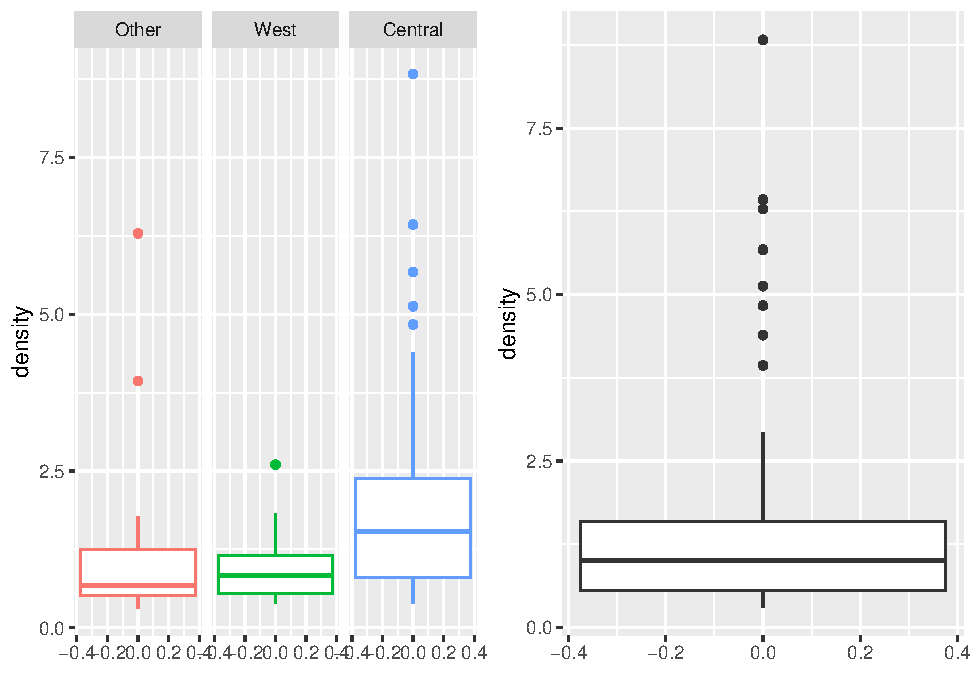
\includegraphics{Bagnard_Gaustad_Hartman_Leung_Lab_3_files/figure-latex/unnamed-chunk-78-1.pdf}

\textbf{Variables not considered}\\
Tax per Capital: Given that we found taxes per capita insignificant from
model 2, we will exclude it from model 3.

We have also chosen not to include other variables from our dataset in
our model:\\
* Urban: We believe the variable ``density'' better explains the same
effects as ``urban'' while also being a continous. We believe a
continous variable is more meaningful rather a binary indicator such as
urban as there may be data points that failed to meet the cutoff for
being defined as urban, but may still see the same effects as being
urban and hence may distort our analysis.\\
* Age and Gender: While age and gender are important demographic
variables, the only variable in our dataset is pctymle which provides
the percentage of young males in the population. However, given that
this variable encompasses both male and young, we may not be able to
discern if age or gender has the larger effect (if any at all).\\
* Judgement: We chose not to include the varibles concerning the
probability of a prison sentence as well as the average sentence as we
believe it is unlikely that potential criminals would have good access
to this information. In addition, local county officials have limited
influence over the decisions of the judiciary system, as they are
separate branches of government.

Our equation for model 3 is as follows:

\[log(CrimeRate) = \beta_0 + \beta_1log(Scaled Wages) + \beta_2log(CriminalJusticeEffectiveness) + \beta_3West + \\
\beta_4Central+ \beta_5log(PolicePerCapita) + \beta_6log(PercentageofMinorities) + \beta_7Density +u\]

\hypertarget{model-3-linear-model}{%
\subsubsection{Model 3 Linear Model}\label{model-3-linear-model}}

\begin{Shaded}
\begin{Highlighting}[]
\NormalTok{model3_initial<-}\KeywordTok{lm}\NormalTok{(logcrmrte }\OperatorTok{~}\StringTok{ }\NormalTok{logScaledWages }\OperatorTok{+}\StringTok{ }\NormalTok{logcrimJustEff  }\OperatorTok{+}\StringTok{  }\NormalTok{west }\OperatorTok{+}\StringTok{ }\NormalTok{central }\OperatorTok{+}
\StringTok{                     }\NormalTok{logpolpc }\OperatorTok{+}\StringTok{ }\NormalTok{logpctmin80 }\OperatorTok{+}\StringTok{ }\NormalTok{density, }\DataTypeTok{data =}\NormalTok{ dfCrime)}
\KeywordTok{coeftest}\NormalTok{(model3_initial, }\DataTypeTok{vcov=}\NormalTok{vcovHC)}
\end{Highlighting}
\end{Shaded}

\begin{verbatim}

t test of coefficients:

                Estimate Std. Error t value  Pr(>|t|)    
(Intercept)    -9.082572   4.191510 -2.1669 0.0331444 *  
logScaledWages  1.146807   0.603082  1.9016 0.0607384 .  
logcrimJustEff -0.419923   0.105971 -3.9626 0.0001575 ***
west           -0.203700   0.204469 -0.9962 0.3220650    
central        -0.152719   0.096049 -1.5900 0.1156807    
logpolpc        0.253456   0.188526  1.3444 0.1825244    
logpctmin80     0.192875   0.090492  2.1314 0.0360495 *  
density         0.078001   0.030980  2.5178 0.0137565 *  
---
Signif. codes:  0 '***' 0.001 '**' 0.01 '*' 0.05 '.' 0.1 ' ' 1
\end{verbatim}

We note from the the summary above that west and central are no longer
statistically significant to the model, but the inclusion of logpctmin80
and density are significant at the 99\% confidence level or better. It
appears that after controlling for the minority percentage and density,
we can better explain the variation between counties rather than purely
based on their geographic location and we thus remove the latter 2
variables from our model. We confirm by checking whether we have joint
signifcance of west and central below.

\begin{Shaded}
\begin{Highlighting}[]
\KeywordTok{linearHypothesis}\NormalTok{(model3_initial,}\KeywordTok{c}\NormalTok{(}\StringTok{"west=0"}\NormalTok{,}\StringTok{"central=0"}\NormalTok{), }\DataTypeTok{vcov=}\NormalTok{vcovHC)}
\end{Highlighting}
\end{Shaded}

\begin{verbatim}
## Linear hypothesis test
## 
## Hypothesis:
## west = 0
## central = 0
## 
## Model 1: restricted model
## Model 2: logcrmrte ~ logScaledWages + logcrimJustEff + west + central + 
##     logpolpc + logpctmin80 + density
## 
## Note: Coefficient covariance matrix supplied.
## 
##   Res.Df Df      F Pr(>F)
## 1     84                 
## 2     82  2 1.3521 0.2644
\end{verbatim}

Our revised equation for model 3 thus becomes:
\[log(CrimeRate) = \beta_0 + \beta_1log(UnweightedAverageWage) + \beta_2log(CriminalJusticeEffectiveness) +  \\ \beta_3log(PolicePerCapita) +\beta_4log(PercentageofMinorities) + \beta_5Density +u\]

\begin{Shaded}
\begin{Highlighting}[]
\NormalTok{model3<-}\KeywordTok{lm}\NormalTok{(logcrmrte }\OperatorTok{~}\StringTok{ }\NormalTok{logcrimJustEff }\OperatorTok{+}\StringTok{ }\NormalTok{logScaledWages }\OperatorTok{+}\StringTok{  }\NormalTok{logpolpc  }
              \OperatorTok{+}\StringTok{ }\NormalTok{logpctmin80 }\OperatorTok{+}\StringTok{ }\NormalTok{density, }\DataTypeTok{data =}\NormalTok{ dfCrime)}
\NormalTok{model3}
\end{Highlighting}
\end{Shaded}

\begin{verbatim}

Call:
lm(formula = logcrmrte ~ logcrimJustEff + logScaledWages + logpolpc + 
    logpctmin80 + density, data = dfCrime)

Coefficients:
   (Intercept)  logcrimJustEff  logScaledWages        logpolpc  
      -8.43468        -0.44161         1.04826         0.26981  
   logpctmin80         density  
       0.25597         0.06707  
\end{verbatim}

\begin{Shaded}
\begin{Highlighting}[]
\KeywordTok{summary}\NormalTok{(model3)}\OperatorTok{$}\NormalTok{adj.r.square}
\end{Highlighting}
\end{Shaded}

\begin{verbatim}
## [1] 0.7213662
\end{verbatim}

From the Residuals vs Leverage plot below, we also note that there are
despite some data points have more leverage than others, no major
outliers that have significant influence on our model as measured by no
points having a Cook's distance \textgreater{} 0.5.

\begin{Shaded}
\begin{Highlighting}[]
\KeywordTok{plot}\NormalTok{(model3,}\DataTypeTok{which=}\DecValTok{5}\NormalTok{)}
\end{Highlighting}
\end{Shaded}

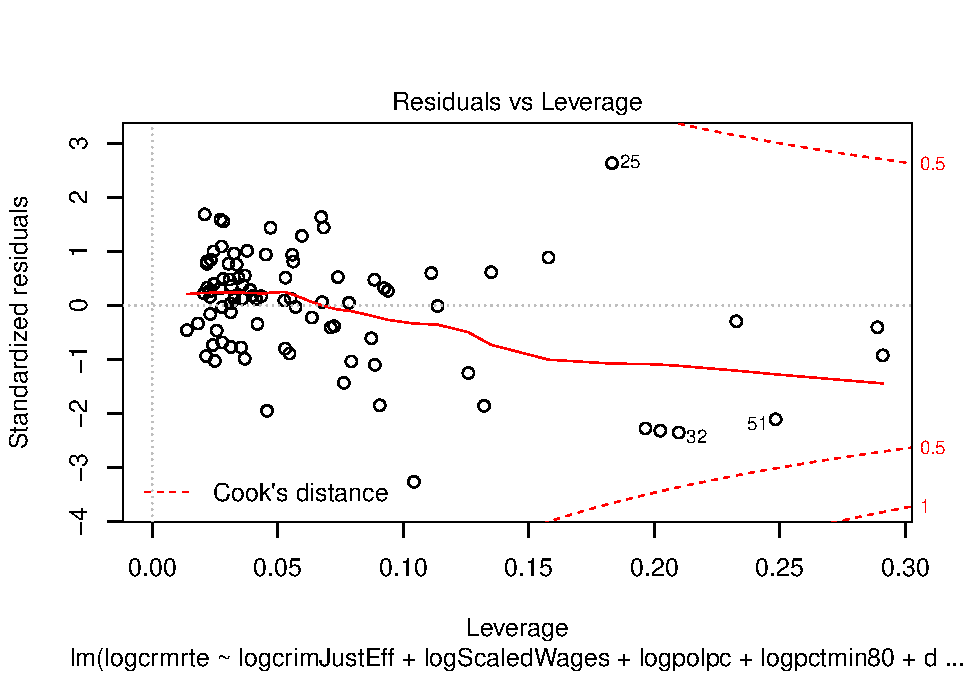
\includegraphics{Bagnard_Gaustad_Hartman_Leung_Lab_3_files/figure-latex/unnamed-chunk-83-1.pdf}

\textbf{Model 3 CLM Assumptions:}

\begin{itemize}
\item
  \textbf{MLR1 and 2}: Discussed earlier.
\item
  \textbf{MLR3} No perfect multicollinearity: We demonstrate that our
  independent variables are not perfectly multicollinear using the VIF
  function, and note that all of our variance inflation factors are less
  than 5.
\end{itemize}

\begin{Shaded}
\begin{Highlighting}[]
\KeywordTok{vif}\NormalTok{(model3)}
\end{Highlighting}
\end{Shaded}

\begin{verbatim}
## logcrimJustEff logScaledWages       logpolpc    logpctmin80        density 
##       1.332313       1.730692       1.326710       1.046384       2.060321
\end{verbatim}

\begin{itemize}
\tightlist
\item
  \textbf{MLR4'} Zero Conditional Mean: From the residual vs.~fitted
  chart below, we see that the mean of the residuals mostly lie along 0,
  except towards the right side of our chart where there are fewer data
  points. We can reasonably conclude that we satisfy MLR4.
\end{itemize}

\begin{Shaded}
\begin{Highlighting}[]
\KeywordTok{plot}\NormalTok{(model3, }\DataTypeTok{which =} \DecValTok{1}\NormalTok{)}
\end{Highlighting}
\end{Shaded}

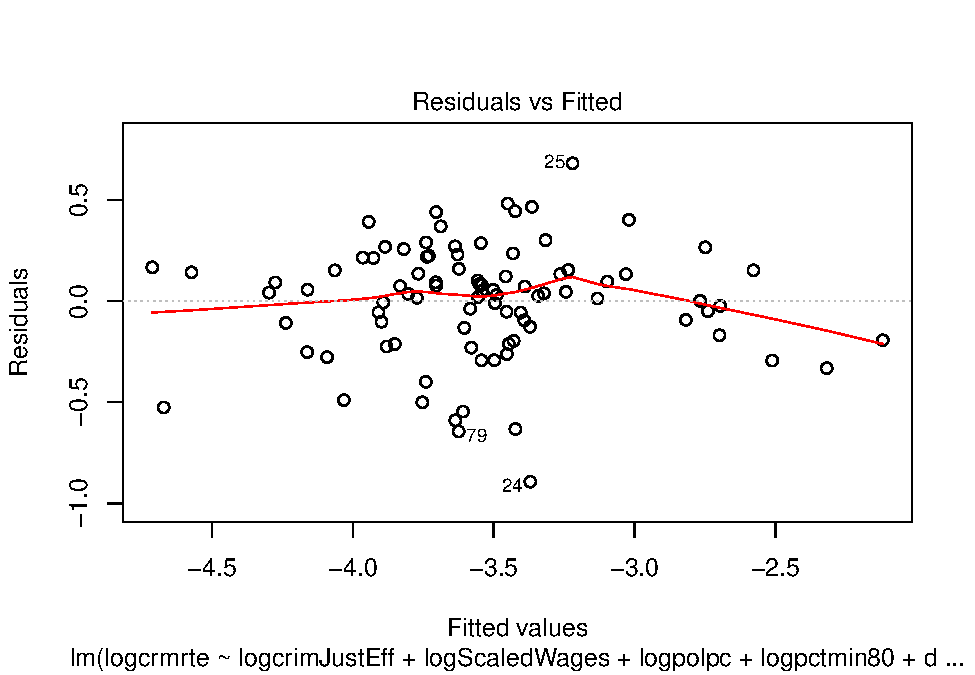
\includegraphics{Bagnard_Gaustad_Hartman_Leung_Lab_3_files/figure-latex/unnamed-chunk-85-1.pdf}

\begin{itemize}
\tightlist
\item
  \textbf{MLR5'} Spherical errors: We note from the residuals vs fitted
  chart above that we have some evidence of heteroscedasticity, since
  there are less datapoints on both the left and right of the chart. As
  a result, we use the vcovHC method to estimate a robust
  variance-covariance matrix using White and Huber's method and generate
  coefficients that are robust to heteroscedasticity.
\end{itemize}

\begin{Shaded}
\begin{Highlighting}[]
\KeywordTok{coeftest}\NormalTok{(model3, }\DataTypeTok{vcov=}\NormalTok{vcovHC)}
\end{Highlighting}
\end{Shaded}

\begin{verbatim}

t test of coefficients:

                Estimate Std. Error t value  Pr(>|t|)    
(Intercept)    -8.434684   4.547050 -1.8550   0.06711 .  
logcrimJustEff -0.441605   0.101261 -4.3611 3.653e-05 ***
logScaledWages  1.048265   0.654226  1.6023   0.11284    
logpolpc        0.269809   0.190255  1.4181   0.15985    
logpctmin80     0.255969   0.042151  6.0727 3.521e-08 ***
density         0.067068   0.035044  1.9138   0.05905 .  
---
Signif. codes:  0 '***' 0.001 '**' 0.01 '*' 0.05 '.' 0.1 ' ' 1
\end{verbatim}

\begin{itemize}
\tightlist
\item
  \textbf{MLR6'} Normality of errors: From the qqplot below, we see that
  the residuals in our model follow a fairly normal distribution. In
  addition, since we have a large sample size of 90 datapoints, we can
  rely on a version of the central limit theorem to assume normally
  distributed errors.
\end{itemize}

\begin{Shaded}
\begin{Highlighting}[]
\KeywordTok{plot}\NormalTok{(model3,}\DataTypeTok{which=}\DecValTok{2}\NormalTok{)}
\end{Highlighting}
\end{Shaded}

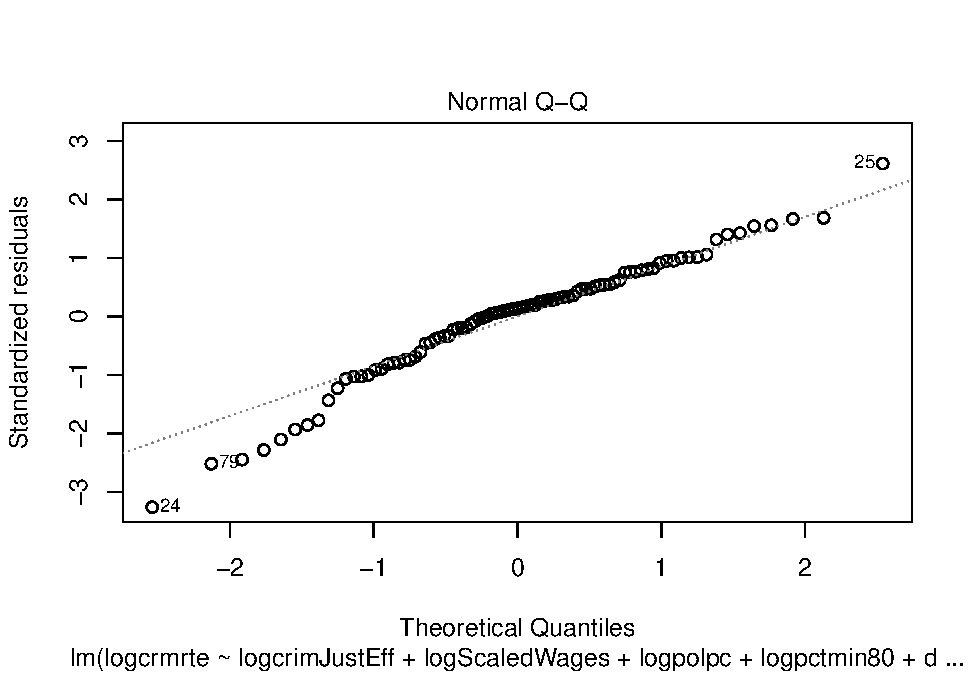
\includegraphics{Bagnard_Gaustad_Hartman_Leung_Lab_3_files/figure-latex/unnamed-chunk-87-1.pdf}

By satisfying these assumptions, we can expect that our coefficients are
approaching the true parameter values in probability.

\hypertarget{model-3-interpretation}{%
\subsubsection{Model 3 Interpretation}\label{model-3-interpretation}}

The model shows a good fit, with an adjusted R-squared of 0.72, meaning
that the model explains 72\% of the variation in crime with less
variables than model 2.

After accounting for coefficients that are robust to heteroscedasticity,
we note only three them have individual statistical significance at the
95\% level or better. These are criminal justice efficiency, minority
percentages and density. However, running a F-test on the other two
variables logpolpc and logScaledWages show that jointly they are still
significant for our model, and thus we will include them for final
analysis.

\begin{Shaded}
\begin{Highlighting}[]
\KeywordTok{linearHypothesis}\NormalTok{(model3,}\KeywordTok{c}\NormalTok{(}\StringTok{"logpolpc=0"}\NormalTok{,}\StringTok{"logScaledWages=0"}\NormalTok{), }\DataTypeTok{vcov=}\NormalTok{vcovHC)}
\end{Highlighting}
\end{Shaded}

\begin{verbatim}
## Linear hypothesis test
## 
## Hypothesis:
## logpolpc = 0
## logScaledWages = 0
## 
## Model 1: restricted model
## Model 2: logcrmrte ~ logcrimJustEff + logScaledWages + logpolpc + logpctmin80 + 
##     density
## 
## Note: Coefficient covariance matrix supplied.
## 
##   Res.Df Df      F Pr(>F)   
## 1     86                    
## 2     84  2 4.9848  0.009 **
## ---
## Signif. codes:  0 '***' 0.001 '**' 0.01 '*' 0.05 '.' 0.1 ' ' 1
\end{verbatim}

\textbf{Interpretation of coefficients (Assuming ceterus paribus):}

\begin{Shaded}
\begin{Highlighting}[]
\KeywordTok{coeftest}\NormalTok{(model3, }\DataTypeTok{vcov=}\NormalTok{vcovHC)}
\end{Highlighting}
\end{Shaded}

\begin{verbatim}

t test of coefficients:

                Estimate Std. Error t value  Pr(>|t|)    
(Intercept)    -8.434684   4.547050 -1.8550   0.06711 .  
logcrimJustEff -0.441605   0.101261 -4.3611 3.653e-05 ***
logScaledWages  1.048265   0.654226  1.6023   0.11284    
logpolpc        0.269809   0.190255  1.4181   0.15985    
logpctmin80     0.255969   0.042151  6.0727 3.521e-08 ***
density         0.067068   0.035044  1.9138   0.05905 .  
---
Signif. codes:  0 '***' 0.001 '**' 0.01 '*' 0.05 '.' 0.1 ' ' 1
\end{verbatim}

Positive coefficients:\\
* Police presence: If we increase police per capita by 1 percent, we
expect the crime rate to increase by around 0.28\%.\\
* scaledWages: If we increase wages by 1 percent, we expect the crime
rate to also increase by roughly 1\%.\\
* Density: If we increase density by 100 people per square mile, we
expect the crime rate to increase by approximately 6.9\%.\\
* Percentage of minorities: If the percentage of minorities increase by
1\%, we expect the crime rate to increase by 0.25\%.

Negative coefficients:\\
* Criminal justice efficiency: If we increase the criminal justice
efficiency by 1\%, we expect the crime rate to decrease by around
0.43\%.

Of these different variables, we should pay particular attention to
density given its large practical effect and statistical significance,
which we address in our policy recommendations in the next section.

\hypertarget{comparison-of-regression-models}{%
\subsection{Comparison of Regression
Models}\label{comparison-of-regression-models}}

\begin{Shaded}
\begin{Highlighting}[]
\CommentTok{#*** Function to convert coeftest results object into data frame}
\NormalTok{ctdf=}\ControlFlowTok{function}\NormalTok{(x)\{}
\NormalTok{  rt=}\KeywordTok{list}\NormalTok{()                             }\CommentTok{# generate empty results list}
  \ControlFlowTok{for}\NormalTok{(c }\ControlFlowTok{in} \DecValTok{1}\OperatorTok{:}\KeywordTok{dim}\NormalTok{(x)[}\DecValTok{2}\NormalTok{]) rt[[c]]=x[,c]   }\CommentTok{# writes column values of x to list}
\NormalTok{  rt=}\KeywordTok{as.data.frame}\NormalTok{(rt)                  }\CommentTok{# converts list to data frame object}
  \KeywordTok{names}\NormalTok{(rt)=}\KeywordTok{names}\NormalTok{(x[}\DecValTok{1}\NormalTok{,])                }\CommentTok{# assign correct column names}
\NormalTok{  rt[,}\StringTok{"sig"}\NormalTok{]=}\KeywordTok{symnum}\NormalTok{(rt}\OperatorTok{$}\StringTok{`}\DataTypeTok{Pr(>|z|)}\StringTok{`}\NormalTok{, }\DataTypeTok{corr =} \OtherTok{FALSE}\NormalTok{, }\DataTypeTok{na =} \OtherTok{FALSE}\NormalTok{,}
                    \DataTypeTok{cutpoints =} \KeywordTok{c}\NormalTok{(}\DecValTok{0}\NormalTok{, }\FloatTok{0.001}\NormalTok{, }\FloatTok{0.01}\NormalTok{, }\FloatTok{0.05}\NormalTok{, }\FloatTok{0.1}\NormalTok{, }\DecValTok{1}\NormalTok{),}
                    \DataTypeTok{symbols =} \KeywordTok{c}\NormalTok{(}\StringTok{"***"}\NormalTok{, }\StringTok{"**"}\NormalTok{, }\StringTok{"*"}\NormalTok{, }\StringTok{"."}\NormalTok{, }\StringTok{" "}\NormalTok{))}
  \KeywordTok{return}\NormalTok{(rt)}
\NormalTok{\}}
\CommentTok{# Get vectors of robust standard errors from the coeftest output}
\NormalTok{se.model1 <-}\StringTok{ }\KeywordTok{ctdf}\NormalTok{(}\KeywordTok{coeftest}\NormalTok{(model1, }\DataTypeTok{vcov=}\NormalTok{vcovHC))[,}\StringTok{"Std. Error"}\NormalTok{]}
\NormalTok{se.model2 <-}\StringTok{ }\KeywordTok{ctdf}\NormalTok{(}\KeywordTok{coeftest}\NormalTok{(model2, }\DataTypeTok{vcov=}\NormalTok{vcovHC))[,}\StringTok{"Std. Error"}\NormalTok{]}
\NormalTok{se.model3 <-}\StringTok{ }\KeywordTok{ctdf}\NormalTok{(}\KeywordTok{coeftest}\NormalTok{(model3, }\DataTypeTok{vcov=}\NormalTok{vcovHC))[,}\StringTok{"Std. Error"}\NormalTok{]}

\CommentTok{# Pass the standard errors into stargazer}
\KeywordTok{stargazer}\NormalTok{(model1, model2, model3, }\DataTypeTok{type =} \StringTok{"text"}\NormalTok{, }\DataTypeTok{omit.stat =} \StringTok{"f"}\NormalTok{,}
          \DataTypeTok{se =} \KeywordTok{list}\NormalTok{(se.model1, se.model2, se.model3),}
          \DataTypeTok{star.cutoffs =} \KeywordTok{c}\NormalTok{(}\FloatTok{0.05}\NormalTok{, }\FloatTok{0.01}\NormalTok{, }\FloatTok{0.001}\NormalTok{))}
\end{Highlighting}
\end{Shaded}

\begin{verbatim}

===================================================================
                                  Dependent variable:              
                    -----------------------------------------------
                                       logcrmrte                   
                          (1)             (2)             (3)      
-------------------------------------------------------------------
logScaledWages         1.993***         1.191*           1.048     
                        (0.489)         (0.474)         (0.654)    
                                                                   
logcrimJustEff         -0.479***       -0.423***       -0.442***   
                        (0.105)         (0.107)         (0.101)    
                                                                   
logpolpc                                0.562*           0.270     
                                        (0.253)         (0.190)    
                                                                   
west                   -0.592***        -5.953*                    
                        (0.102)         (2.976)                    
                                                                   
central                -0.242**          1.002                     
                        (0.081)         (1.435)                    
                                                                   
logtaxpc                                -0.150                     
                                        (0.190)                    
                                                                   
logpolpc:west                           -0.825                     
                                        (0.455)                    
                                                                   
logpolpc:central                         0.186                     
                                        (0.220)                    
                                                                   
logpctmin80                                            0.256***    
                                                        (0.042)    
                                                                   
density                                                  0.067     
                                                        (0.035)    
                                                                   
Constant              -15.827***        -6.902          -8.435     
                        (2.672)         (3.602)         (4.547)    
                                                                   
-------------------------------------------------------------------
Observations              90              90              90       
R2                       0.650           0.727           0.737     
Adjusted R2              0.633           0.700           0.721     
Residual Std. Error 0.332 (df = 85) 0.300 (df = 81) 0.290 (df = 84)
===================================================================
Note:                                 *p<0.05; **p<0.01; ***p<0.001
\end{verbatim}

\hypertarget{interpretation-and-discussion}{%
\subsubsection{Interpretation and
Discussion}\label{interpretation-and-discussion}}

Comparing the 3 models, we see that by increasing the complexity of our
model specifications we have increased the fit of our model. The
adjusted \(R^2\) value has steadily increased from 63\% to nearly 73\%
between model 1 and 3, indicating that we were able to explain
approximately 10\% more of the variation in our model. At the same time,
our overall standard errors (which have been adjusted to account for
hetereoscedacity) have also decreased.

\begin{itemize}
\tightlist
\item
  logScaledWages: As we dived deeper into our analysis of independent
  variables that operationalized economic conditions, we note that the
  scaled average weekly wage has decreased both in terms of its
  practical significance (as measured by the magnitude of the
  coefficient) as well as its statistical significance. This indicates
  that as we controlled for additional covariates, the effect of wages
  are not as pronounced. In addition, the size of our standard errors
  increased from model 1 to 3. As a result, we do not believe that the
  average wage is a good determinant of crime.\\
\item
  logcrimJustEff: Criminal justice effectiveness has maintained
  relatively stable across all 3 models with a negative coefficient of
  approximately -0.4 to -0.5, holding constant the effect for other
  covariates. It also maintained high statistical significance at the
  99.9\% confidence level and has relatively low standard errors across
  the models. Hence, criminal justice effectiveness is an important
  deterrent of crime, having the ability to lower the crime rate by
  0.4\% to 0.5\% per 1\% increase in convictions per crime.\\
\item
  logpolpc: Police per capita was statistically significant in the model
  2, but once we controlled for density and the minority percentage, it
  became statistically insignificant in model 3. However, the higher
  joint significance with wage shows there is justification that merits
  further study.
\item
  West and Central: The two regions were statistically significant in
  model 1, but became less significant in the later two models once we
  started controlling for other variables. However, the western region
  in particular consistently demonstrated a negative effect on the crime
  rate and we believe that it would be meaningful for researchers to
  pursue further analysis with additional data beyond our existing
  dataset.\\
\item
  Interactions between police presence and regions: These interactions
  were deemed not statistically significant and removed for model 3.\\
\item
  Tax per capita: Taxes did not appear to be practically or
  statistically significant.\\
\item
  Percentage of minorities: This variable was highly statistically
  significant, and its inclusion helped explain some of the variation in
  the different regions. In addition, compared to the other variables,
  it has a relatively low residual standard error. While we think that
  the percentage of minorities is an important consideration for crime
  rates, but due to the fact that is opertionalizes a difficult
  demographic concept (racism), it is unlikely that a high minority
  percentage in itself is a cause of crime.\\
\item
  Density: Density is statistically significant at the 95\% confidence
  level and represents a large practical effect as an increase in 100
  people per square mile leads to approximately 6.9\% increase in the
  crime rate.
\end{itemize}

From the analysis of the coefficients, as well as their practical and
statistical significance, we highlight specifically 1) Criminal Justice
Effectiveness, 2) Percentage of Minorities and 3) Population density as
the most important factors in explaining crime. Criminal justice
effectiveness can be increased by either increasing convictions or
decreasing the number of crimes, while the two demographic variables
indicate the areas of focus for policy recommendations. We also note
that the western region and possible varations of policing style is
deserving of further research and analysis beyond the scope of this
paper.

\hypertarget{ommitted-variables}{%
\subsubsection{Ommitted Variables}\label{ommitted-variables}}

\begin{longtable}[]{@{}l@{}}
\toprule
Expected correlation between omitted and included
variables\tabularnewline
\midrule
\endhead
\bottomrule
\end{longtable}

\begin{longtable}[]{@{}llll@{}}
\toprule
\begin{minipage}[b]{0.18\columnwidth}\raggedright
Omitted Variable\strut
\end{minipage} & \begin{minipage}[b]{0.19\columnwidth}\raggedright
Crime Rate (\(B_k\))\strut
\end{minipage} & \begin{minipage}[b]{0.31\columnwidth}\raggedright
Criminal Justice Effectiveness\strut
\end{minipage} & \begin{minipage}[b]{0.20\columnwidth}\raggedright
Economic Conditions\strut
\end{minipage}\tabularnewline
\midrule
\endhead
\begin{minipage}[t]{0.18\columnwidth}\raggedright
Education\strut
\end{minipage} & \begin{minipage}[t]{0.19\columnwidth}\raggedright
-\strut
\end{minipage} & \begin{minipage}[t]{0.31\columnwidth}\raggedright
unknown\strut
\end{minipage} & \begin{minipage}[t]{0.20\columnwidth}\raggedright
+\strut
\end{minipage}\tabularnewline
\begin{minipage}[t]{0.18\columnwidth}\raggedright
Social Services\strut
\end{minipage} & \begin{minipage}[t]{0.19\columnwidth}\raggedright
-\strut
\end{minipage} & \begin{minipage}[t]{0.31\columnwidth}\raggedright
unknown\strut
\end{minipage} & \begin{minipage}[t]{0.20\columnwidth}\raggedright
unknown\strut
\end{minipage}\tabularnewline
\begin{minipage}[t]{0.18\columnwidth}\raggedright
Unemployment\strut
\end{minipage} & \begin{minipage}[t]{0.19\columnwidth}\raggedright
+\strut
\end{minipage} & \begin{minipage}[t]{0.31\columnwidth}\raggedright
unknown\strut
\end{minipage} & \begin{minipage}[t]{0.20\columnwidth}\raggedright
-\strut
\end{minipage}\tabularnewline
\begin{minipage}[t]{0.18\columnwidth}\raggedright
Inequality\strut
\end{minipage} & \begin{minipage}[t]{0.19\columnwidth}\raggedright
+\strut
\end{minipage} & \begin{minipage}[t]{0.31\columnwidth}\raggedright
unknown\strut
\end{minipage} & \begin{minipage}[t]{0.20\columnwidth}\raggedright
-\strut
\end{minipage}\tabularnewline
\begin{minipage}[t]{0.18\columnwidth}\raggedright
Gang Activity\strut
\end{minipage} & \begin{minipage}[t]{0.19\columnwidth}\raggedright
+\strut
\end{minipage} & \begin{minipage}[t]{0.31\columnwidth}\raggedright
-\strut
\end{minipage} & \begin{minipage}[t]{0.20\columnwidth}\raggedright
-\strut
\end{minipage}\tabularnewline
\begin{minipage}[t]{0.18\columnwidth}\raggedright
Gov't Spending\strut
\end{minipage} & \begin{minipage}[t]{0.19\columnwidth}\raggedright
-\strut
\end{minipage} & \begin{minipage}[t]{0.31\columnwidth}\raggedright
+\strut
\end{minipage} & \begin{minipage}[t]{0.20\columnwidth}\raggedright
+\strut
\end{minipage}\tabularnewline
\bottomrule
\end{longtable}

The 5 major identified ommited variables are shown above.

\begin{itemize}
\tightlist
\item
  Education is an important variable because of demographic insights it
  provides. First, adults with higher education are less likely to
  participate in Crime and are more likely to have better economic
  opportunity. Second, a strong school system is also likely correlated
  with less youth crime. Because of these expected correlations we are
  likely overestimating the economic conditions coefficient estimate.\\
\item
  Available Social Services could also lower crime. Citizens with strong
  social services support have more options to get help when they lack
  means for purchasing basic life needs. However this is more difficult
  to predict, as some social service projects, like homeless shelters,
  could lead to more criminal activity.\\
\item
  Unemployment is used as an important indicator of economic health and
  opportunity. This is would be highly correlated to economic conditions
  variables like sum of wages. This indicator variable if added to the
  model would decrease the magnitude of the sum of wage means
  coefficient estimate.\\
\item
  Economic Inequality may also increase the crime rate as it may provide
  incentives for certain types of crime such as theft, kidnapping or
  extortion by people who have less economic means on those who have
  more economic means. As discussed in model 1, it is possible that mean
  wage is correlated to inequality, which explains why wages positively
  correlate to crime in model 1. As we add more regressors in later
  models, this effect is limited. Likely because inequality is better
  correlated to these new regressors like density and minority
  population.\\
\item
  Gang or Organized Crime is a special case of crime that contains
  unique causes. It is expected that it would be negatively correlated
  with criminal justice effectiveness as large social pressures prevent
  witnesses from supporting prosecution. Gang crime is also negatively
  correlated with economic conditions. From these assumed correlations,
  we can say that criminal justice effectiveness and economic conditions
  are both underestimated compared to including a gang activity
  operationalized variable in the model.\\
\item
  Government spending: Our analysis showed that local tax revenues per
  capita were not an important variable and part of this may be because
  tax revenues and government spending may not actually be strongly
  correlated. Effective government spending could help boost criminal
  justice effectiveness as well as local economic conditions, including
  some of the variables noted above such as education, social services
  and inequality.
\end{itemize}

\hypertarget{conclusion}{%
\section{Conclusion}\label{conclusion}}

\hypertarget{policy-recommendations}{%
\subsection{Policy Recommendations}\label{policy-recommendations}}

We have shown in this report 3 different models that seek to explain and
model changes in the crime rate in North Carolina in 1980. We start with
the fundamental premise that crime is affected by criminal justice
efficiency, economic conditions and regional differences, and further
develop our definition of these key explanatory variables which each new
model. We propose the following recommendations on crime policy for
local political candidates.

\begin{itemize}
  \item Crime is more prevalent in places with higher population density and higher minority populations. Those seeking election in these areas should make crime reduction an important part of their message. Note that we do not offer recommendations on how important the issue of crime is relative to other issues as that is beyond the scope of our analysis.
  \item Increase the number of rightful convictions by providing appropriate staffing and resources to local law enforcement and legal system. In highly populated areas, this could include increasing public safety infrastructure (such as security cameras) and reducing police response times. With the right resources, density can be used against potential criminals and act as a deterrent to crime. However, note that simply increasing the number of police will not necessarily lead to an increase in criminal justice effectiveness.
  \item Provide additional support for areas with high minority populations, by conducting further studies on our ommitted variables. These could come in different forms such as better access to education, social support services or by reducing income equality. Our analysis has shown that average wages do not have a strong relationship with crime so it is important to get to the root of why these areas suffer from higher crime rates in order to provide more concrete recommendations to reduce crime in these areas.
    \item Provide racial subconscious bias training to local law enforcement and judiciary officials to reduce the number of wrongful arrests or incidents labelled as potential crimes.
\end{itemize}

\hypertarget{recommendations-for-future-research}{%
\subsection{Recommendations for Future
Research}\label{recommendations-for-future-research}}

Our findings can be further strengthed by studying the ommitted
variables we have identified, the differences in the western region, as
well as a time-panel of data that shows how criminal data and our
independent variables change over time. Political candidates who are
interested in making crime reduction an important campaign promise
should consider funding these studies.

\hypertarget{appendix}{%
\section{Appendix}\label{appendix}}

We include below additional network correlation plots seperated by
region and metro attributes. We drew further inspiration from these
plots for policy recommendations and variables to test that are be
influenced by the regional and density variations.

\begin{Shaded}
\begin{Highlighting}[]
\KeywordTok{options}\NormalTok{(}\DataTypeTok{repr.plot.width=}\DecValTok{8}\NormalTok{, }\DataTypeTok{repr.plot.height=}\DecValTok{4}\NormalTok{)}
\CommentTok{#myData<-myData[, c("crmrte", "prbarr", "prbconv", "prbpris", "avgsen", "polpc", "density", "taxpc",}
\CommentTok{#           "pctmin80", "wcon", "wtuc", "wtrd", "wfir", "wser", "wmfg", "wfed", "wsta", "wloc",}
\CommentTok{#           "mix", "pctymle")]}
\NormalTok{myData<-dfCrime }\OperatorTok\StringTok{ }\KeywordTok{filter}\NormalTok{(other}\OperatorTok{==}\DecValTok{1}\NormalTok{)}
\NormalTok{myData<-myData[, }\KeywordTok{c}\NormalTok{(}\StringTok{"crmrte"}\NormalTok{, }\StringTok{"prbarr"}\NormalTok{, }\StringTok{"prbconv"}\NormalTok{, }\StringTok{"prbpris"}\NormalTok{, }\StringTok{"avgsen"}\NormalTok{, }\StringTok{"polpc"}\NormalTok{, }\StringTok{"density"}\NormalTok{, }\StringTok{"taxpc"}\NormalTok{,}
          \StringTok{"pctmin80"}\NormalTok{, }\StringTok{"wcon"}\NormalTok{, }\StringTok{"wtuc"}\NormalTok{, }\StringTok{"wtrd"}\NormalTok{, }\StringTok{"wfir"}\NormalTok{, }\StringTok{"wser"}\NormalTok{, }\StringTok{"wmfg"}\NormalTok{, }\StringTok{"wfed"}\NormalTok{, }\StringTok{"wsta"}\NormalTok{, }\StringTok{"wloc"}\NormalTok{,}
          \StringTok{"mix"}\NormalTok{, }\StringTok{"pctymle"}\NormalTok{)]}
\NormalTok{r0 <-}\StringTok{ }\NormalTok{myData }\OperatorTok\StringTok{ }\KeywordTok{correlate}\NormalTok{() }\OperatorTok\StringTok{ }\KeywordTok{network_plot}\NormalTok{(}\DataTypeTok{min_cor=}\NormalTok{.}\DecValTok{25}\NormalTok{)}
\end{Highlighting}
\end{Shaded}

\begin{verbatim}

Correlation method: 'pearson'
Missing treated using: 'pairwise.complete.obs'
\end{verbatim}

\begin{Shaded}
\begin{Highlighting}[]
\NormalTok{myData<-dfCrime }\OperatorTok\StringTok{ }\KeywordTok{filter}\NormalTok{(central}\OperatorTok{==}\DecValTok{1}\NormalTok{)}
\NormalTok{myData<-myData[, }\KeywordTok{c}\NormalTok{(}\StringTok{"crmrte"}\NormalTok{, }\StringTok{"prbarr"}\NormalTok{, }\StringTok{"prbconv"}\NormalTok{, }\StringTok{"prbpris"}\NormalTok{, }\StringTok{"avgsen"}\NormalTok{, }\StringTok{"polpc"}\NormalTok{, }\StringTok{"density"}\NormalTok{, }\StringTok{"taxpc"}\NormalTok{,}
          \StringTok{"pctmin80"}\NormalTok{, }\StringTok{"wcon"}\NormalTok{, }\StringTok{"wtuc"}\NormalTok{, }\StringTok{"wtrd"}\NormalTok{, }\StringTok{"wfir"}\NormalTok{, }\StringTok{"wser"}\NormalTok{, }\StringTok{"wmfg"}\NormalTok{, }\StringTok{"wfed"}\NormalTok{, }\StringTok{"wsta"}\NormalTok{, }\StringTok{"wloc"}\NormalTok{,}
          \StringTok{"mix"}\NormalTok{, }\StringTok{"pctymle"}\NormalTok{)]}
\NormalTok{r1 <-}\StringTok{ }\NormalTok{myData }\OperatorTok\StringTok{ }\KeywordTok{correlate}\NormalTok{() }\OperatorTok\StringTok{ }\KeywordTok{network_plot}\NormalTok{(}\DataTypeTok{min_cor=}\NormalTok{.}\DecValTok{25}\NormalTok{)}
\end{Highlighting}
\end{Shaded}

\begin{verbatim}

Correlation method: 'pearson'
Missing treated using: 'pairwise.complete.obs'
\end{verbatim}

\begin{Shaded}
\begin{Highlighting}[]
\NormalTok{myData<-dfCrime }\OperatorTok\StringTok{ }\KeywordTok{filter}\NormalTok{(west}\OperatorTok{==}\DecValTok{1}\NormalTok{)}
\NormalTok{myData<-myData[, }\KeywordTok{c}\NormalTok{(}\StringTok{"crmrte"}\NormalTok{, }\StringTok{"prbarr"}\NormalTok{, }\StringTok{"prbconv"}\NormalTok{, }\StringTok{"prbpris"}\NormalTok{, }\StringTok{"avgsen"}\NormalTok{, }\StringTok{"polpc"}\NormalTok{, }\StringTok{"density"}\NormalTok{, }\StringTok{"taxpc"}\NormalTok{,}
          \StringTok{"pctmin80"}\NormalTok{, }\StringTok{"wcon"}\NormalTok{, }\StringTok{"wtuc"}\NormalTok{, }\StringTok{"wtrd"}\NormalTok{, }\StringTok{"wfir"}\NormalTok{, }\StringTok{"wser"}\NormalTok{, }\StringTok{"wmfg"}\NormalTok{, }\StringTok{"wfed"}\NormalTok{, }\StringTok{"wsta"}\NormalTok{, }\StringTok{"wloc"}\NormalTok{,}
          \StringTok{"mix"}\NormalTok{, }\StringTok{"pctymle"}\NormalTok{)]}
\NormalTok{r2 <-}\StringTok{ }\NormalTok{myData }\OperatorTok\StringTok{ }\KeywordTok{correlate}\NormalTok{() }\OperatorTok\StringTok{ }\KeywordTok{network_plot}\NormalTok{(}\DataTypeTok{min_cor=}\NormalTok{.}\DecValTok{25}\NormalTok{)}
\end{Highlighting}
\end{Shaded}

\begin{verbatim}

Correlation method: 'pearson'
Missing treated using: 'pairwise.complete.obs'
\end{verbatim}

\begin{Shaded}
\begin{Highlighting}[]
\KeywordTok{grid.arrange}\NormalTok{(}\KeywordTok{arrangeGrob}\NormalTok{(r1, }\DataTypeTok{bottom =} \StringTok{'Central Region Correlation Plot'}\NormalTok{), }\DataTypeTok{ncol=}\DecValTok{1}\NormalTok{)}
\end{Highlighting}
\end{Shaded}

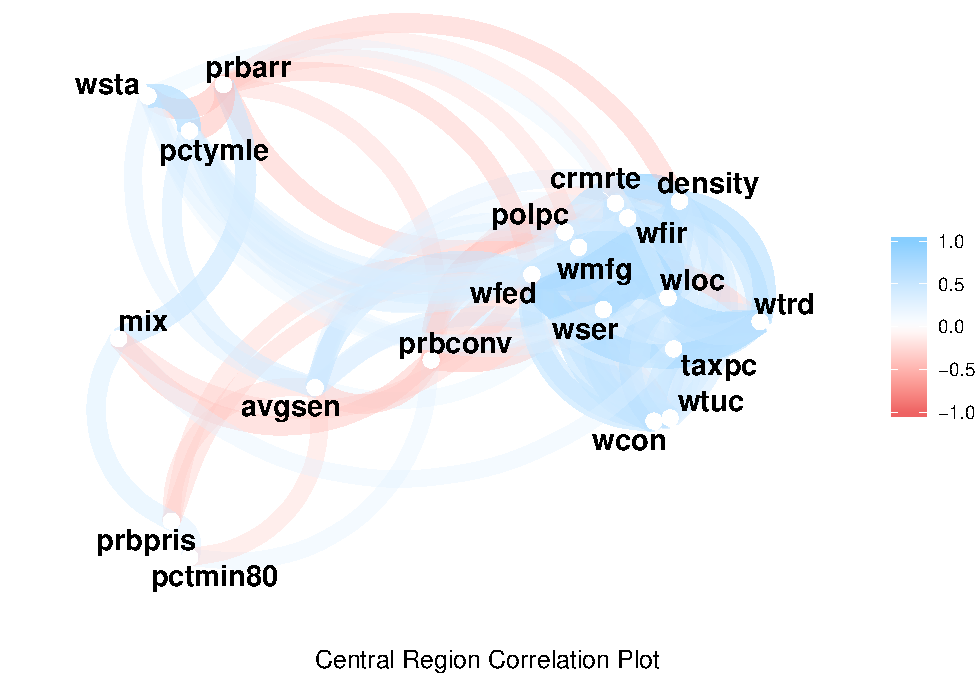
\includegraphics{Bagnard_Gaustad_Hartman_Leung_Lab_3_files/figure-latex/unnamed-chunk-91-1.pdf}

\begin{Shaded}
\begin{Highlighting}[]
\KeywordTok{grid.arrange}\NormalTok{(}\KeywordTok{arrangeGrob}\NormalTok{(r2, }\DataTypeTok{bottom =} \StringTok{'Western Region Correlation Plot'}\NormalTok{), }\DataTypeTok{ncol=}\DecValTok{1}\NormalTok{)}
\end{Highlighting}
\end{Shaded}

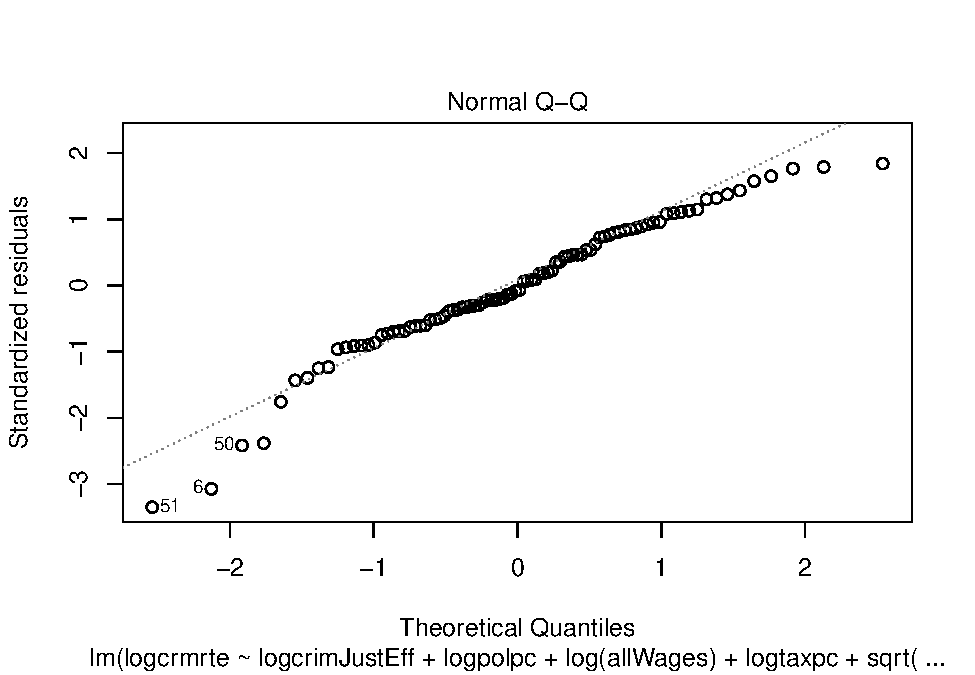
\includegraphics{Bagnard_Gaustad_Hartman_Leung_Lab_3_files/figure-latex/unnamed-chunk-91-2.pdf}

\begin{Shaded}
\begin{Highlighting}[]
\KeywordTok{grid.arrange}\NormalTok{(}\KeywordTok{arrangeGrob}\NormalTok{(r0, }\DataTypeTok{bottom =} \StringTok{'Other Region Correlation Plot'}\NormalTok{), }\DataTypeTok{ncol=}\DecValTok{1}\NormalTok{)}
\end{Highlighting}
\end{Shaded}

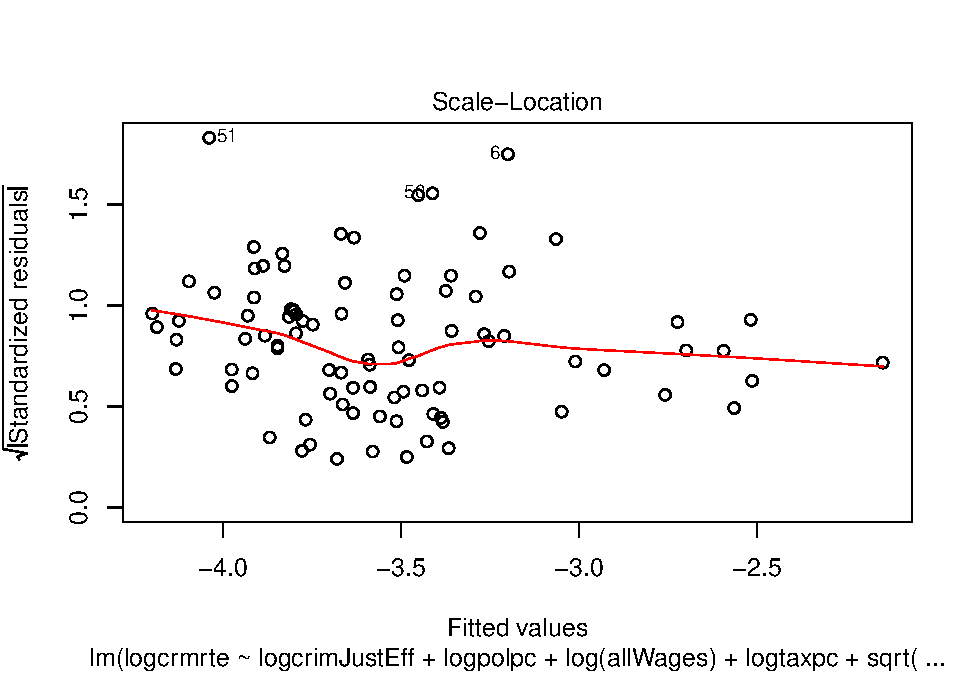
\includegraphics{Bagnard_Gaustad_Hartman_Leung_Lab_3_files/figure-latex/unnamed-chunk-91-3.pdf}

\begin{Shaded}
\begin{Highlighting}[]
\NormalTok{myData<-dfCrime }\OperatorTok\StringTok{ }\KeywordTok{filter}\NormalTok{(urban}\OperatorTok{==}\DecValTok{0}\NormalTok{)}
\NormalTok{myData<-myData[, }\KeywordTok{c}\NormalTok{(}\StringTok{"crmrte"}\NormalTok{, }\StringTok{"prbarr"}\NormalTok{, }\StringTok{"prbconv"}\NormalTok{, }\StringTok{"prbpris"}\NormalTok{, }\StringTok{"avgsen"}\NormalTok{, }\StringTok{"polpc"}\NormalTok{, }\StringTok{"density"}\NormalTok{, }\StringTok{"taxpc"}\NormalTok{,}
          \StringTok{"pctmin80"}\NormalTok{, }\StringTok{"wcon"}\NormalTok{, }\StringTok{"wtuc"}\NormalTok{, }\StringTok{"wtrd"}\NormalTok{, }\StringTok{"wfir"}\NormalTok{, }\StringTok{"wser"}\NormalTok{, }\StringTok{"wmfg"}\NormalTok{, }\StringTok{"wfed"}\NormalTok{, }\StringTok{"wsta"}\NormalTok{, }\StringTok{"wloc"}\NormalTok{,}
          \StringTok{"mix"}\NormalTok{, }\StringTok{"pctymle"}\NormalTok{)]}
\NormalTok{r0 <-}\StringTok{ }\NormalTok{myData }\OperatorTok\StringTok{ }\KeywordTok{correlate}\NormalTok{() }\OperatorTok\StringTok{ }\KeywordTok{network_plot}\NormalTok{(}\DataTypeTok{min_cor=}\NormalTok{.}\DecValTok{25}\NormalTok{)}
\end{Highlighting}
\end{Shaded}

\begin{verbatim}

Correlation method: 'pearson'
Missing treated using: 'pairwise.complete.obs'
\end{verbatim}

\begin{Shaded}
\begin{Highlighting}[]
\NormalTok{myData<-dfCrime }\OperatorTok\StringTok{ }\KeywordTok{filter}\NormalTok{(urban}\OperatorTok{==}\DecValTok{1}\NormalTok{)}
\NormalTok{myData<-myData[, }\KeywordTok{c}\NormalTok{(}\StringTok{"crmrte"}\NormalTok{, }\StringTok{"prbarr"}\NormalTok{, }\StringTok{"prbconv"}\NormalTok{, }\StringTok{"prbpris"}\NormalTok{, }\StringTok{"avgsen"}\NormalTok{, }\StringTok{"polpc"}\NormalTok{, }\StringTok{"density"}\NormalTok{, }\StringTok{"taxpc"}\NormalTok{,}
          \StringTok{"pctmin80"}\NormalTok{, }\StringTok{"wcon"}\NormalTok{, }\StringTok{"wtuc"}\NormalTok{, }\StringTok{"wtrd"}\NormalTok{, }\StringTok{"wfir"}\NormalTok{, }\StringTok{"wser"}\NormalTok{, }\StringTok{"wmfg"}\NormalTok{, }\StringTok{"wfed"}\NormalTok{, }\StringTok{"wsta"}\NormalTok{, }\StringTok{"wloc"}\NormalTok{,}
          \StringTok{"mix"}\NormalTok{, }\StringTok{"pctymle"}\NormalTok{)]}
\NormalTok{r1 <-}\StringTok{ }\NormalTok{myData }\OperatorTok\StringTok{ }\KeywordTok{correlate}\NormalTok{() }\OperatorTok\StringTok{ }\KeywordTok{network_plot}\NormalTok{(}\DataTypeTok{min_cor=}\NormalTok{.}\DecValTok{25}\NormalTok{)}
\end{Highlighting}
\end{Shaded}

\begin{verbatim}

Correlation method: 'pearson'
Missing treated using: 'pairwise.complete.obs'
\end{verbatim}

\begin{Shaded}
\begin{Highlighting}[]
\KeywordTok{grid.arrange}\NormalTok{(}\KeywordTok{arrangeGrob}\NormalTok{(r0, }\DataTypeTok{bottom =} \StringTok{'Non-Urban Correlation Plot'}\NormalTok{), }\DataTypeTok{ncol=}\DecValTok{1}\NormalTok{)}
\end{Highlighting}
\end{Shaded}

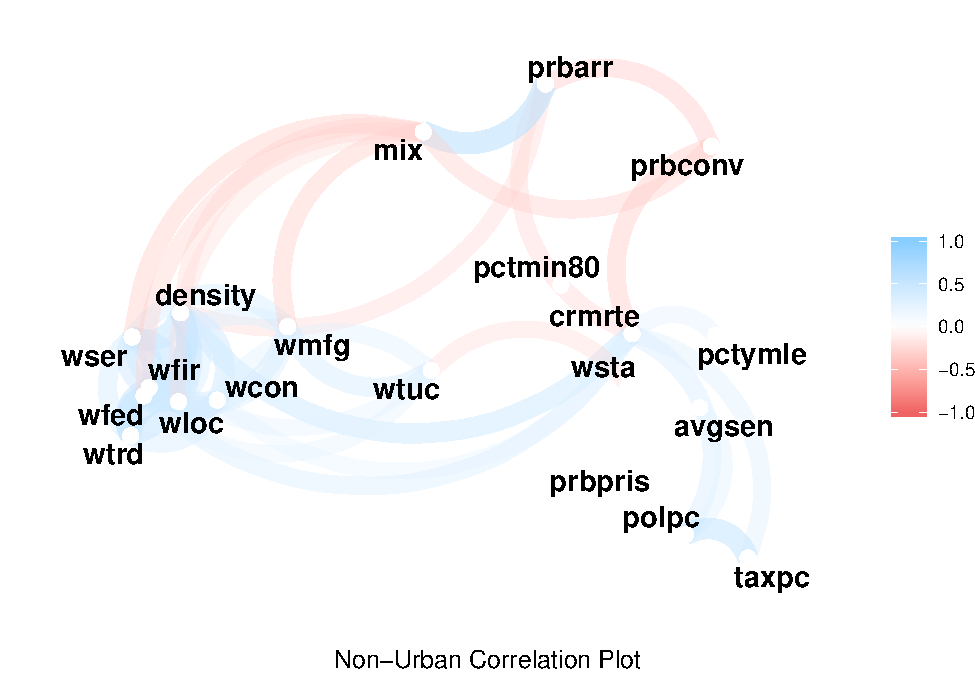
\includegraphics{Bagnard_Gaustad_Hartman_Leung_Lab_3_files/figure-latex/unnamed-chunk-91-4.pdf}

\begin{Shaded}
\begin{Highlighting}[]
\KeywordTok{grid.arrange}\NormalTok{(}\KeywordTok{arrangeGrob}\NormalTok{(r1, }\DataTypeTok{bottom =} \StringTok{'Urban Correlation Plot'}\NormalTok{), }\DataTypeTok{ncol=}\DecValTok{1}\NormalTok{)}
\end{Highlighting}
\end{Shaded}

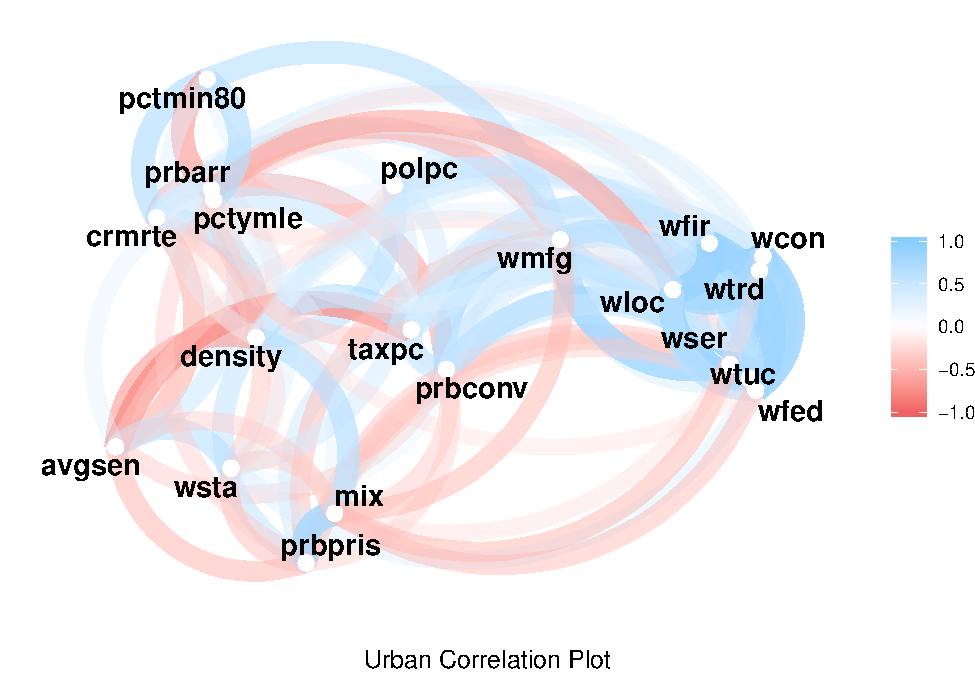
\includegraphics{Bagnard_Gaustad_Hartman_Leung_Lab_3_files/figure-latex/unnamed-chunk-91-5.pdf}


\end{document}
